% Options for packages loaded elsewhere
% Options for packages loaded elsewhere
\PassOptionsToPackage{unicode}{hyperref}
\PassOptionsToPackage{hyphens}{url}
\PassOptionsToPackage{dvipsnames,svgnames,x11names}{xcolor}
%
\documentclass[
  letterpaper,
  DIV=11,
  numbers=noendperiod]{scrreprt}
\usepackage{xcolor}
\usepackage{amsmath,amssymb}
\setcounter{secnumdepth}{5}
\usepackage{iftex}
\ifPDFTeX
  \usepackage[T1]{fontenc}
  \usepackage[utf8]{inputenc}
  \usepackage{textcomp} % provide euro and other symbols
\else % if luatex or xetex
  \usepackage{unicode-math} % this also loads fontspec
  \defaultfontfeatures{Scale=MatchLowercase}
  \defaultfontfeatures[\rmfamily]{Ligatures=TeX,Scale=1}
\fi
\usepackage{lmodern}
\ifPDFTeX\else
  % xetex/luatex font selection
\fi
% Use upquote if available, for straight quotes in verbatim environments
\IfFileExists{upquote.sty}{\usepackage{upquote}}{}
\IfFileExists{microtype.sty}{% use microtype if available
  \usepackage[]{microtype}
  \UseMicrotypeSet[protrusion]{basicmath} % disable protrusion for tt fonts
}{}
\makeatletter
\@ifundefined{KOMAClassName}{% if non-KOMA class
  \IfFileExists{parskip.sty}{%
    \usepackage{parskip}
  }{% else
    \setlength{\parindent}{0pt}
    \setlength{\parskip}{6pt plus 2pt minus 1pt}}
}{% if KOMA class
  \KOMAoptions{parskip=half}}
\makeatother
% Make \paragraph and \subparagraph free-standing
\makeatletter
\ifx\paragraph\undefined\else
  \let\oldparagraph\paragraph
  \renewcommand{\paragraph}{
    \@ifstar
      \xxxParagraphStar
      \xxxParagraphNoStar
  }
  \newcommand{\xxxParagraphStar}[1]{\oldparagraph*{#1}\mbox{}}
  \newcommand{\xxxParagraphNoStar}[1]{\oldparagraph{#1}\mbox{}}
\fi
\ifx\subparagraph\undefined\else
  \let\oldsubparagraph\subparagraph
  \renewcommand{\subparagraph}{
    \@ifstar
      \xxxSubParagraphStar
      \xxxSubParagraphNoStar
  }
  \newcommand{\xxxSubParagraphStar}[1]{\oldsubparagraph*{#1}\mbox{}}
  \newcommand{\xxxSubParagraphNoStar}[1]{\oldsubparagraph{#1}\mbox{}}
\fi
\makeatother

\usepackage{color}
\usepackage{fancyvrb}
\newcommand{\VerbBar}{|}
\newcommand{\VERB}{\Verb[commandchars=\\\{\}]}
\DefineVerbatimEnvironment{Highlighting}{Verbatim}{commandchars=\\\{\}}
% Add ',fontsize=\small' for more characters per line
\usepackage{framed}
\definecolor{shadecolor}{RGB}{241,243,245}
\newenvironment{Shaded}{\begin{snugshade}}{\end{snugshade}}
\newcommand{\AlertTok}[1]{\textcolor[rgb]{0.68,0.00,0.00}{#1}}
\newcommand{\AnnotationTok}[1]{\textcolor[rgb]{0.37,0.37,0.37}{#1}}
\newcommand{\AttributeTok}[1]{\textcolor[rgb]{0.40,0.45,0.13}{#1}}
\newcommand{\BaseNTok}[1]{\textcolor[rgb]{0.68,0.00,0.00}{#1}}
\newcommand{\BuiltInTok}[1]{\textcolor[rgb]{0.00,0.23,0.31}{#1}}
\newcommand{\CharTok}[1]{\textcolor[rgb]{0.13,0.47,0.30}{#1}}
\newcommand{\CommentTok}[1]{\textcolor[rgb]{0.37,0.37,0.37}{#1}}
\newcommand{\CommentVarTok}[1]{\textcolor[rgb]{0.37,0.37,0.37}{\textit{#1}}}
\newcommand{\ConstantTok}[1]{\textcolor[rgb]{0.56,0.35,0.01}{#1}}
\newcommand{\ControlFlowTok}[1]{\textcolor[rgb]{0.00,0.23,0.31}{\textbf{#1}}}
\newcommand{\DataTypeTok}[1]{\textcolor[rgb]{0.68,0.00,0.00}{#1}}
\newcommand{\DecValTok}[1]{\textcolor[rgb]{0.68,0.00,0.00}{#1}}
\newcommand{\DocumentationTok}[1]{\textcolor[rgb]{0.37,0.37,0.37}{\textit{#1}}}
\newcommand{\ErrorTok}[1]{\textcolor[rgb]{0.68,0.00,0.00}{#1}}
\newcommand{\ExtensionTok}[1]{\textcolor[rgb]{0.00,0.23,0.31}{#1}}
\newcommand{\FloatTok}[1]{\textcolor[rgb]{0.68,0.00,0.00}{#1}}
\newcommand{\FunctionTok}[1]{\textcolor[rgb]{0.28,0.35,0.67}{#1}}
\newcommand{\ImportTok}[1]{\textcolor[rgb]{0.00,0.46,0.62}{#1}}
\newcommand{\InformationTok}[1]{\textcolor[rgb]{0.37,0.37,0.37}{#1}}
\newcommand{\KeywordTok}[1]{\textcolor[rgb]{0.00,0.23,0.31}{\textbf{#1}}}
\newcommand{\NormalTok}[1]{\textcolor[rgb]{0.00,0.23,0.31}{#1}}
\newcommand{\OperatorTok}[1]{\textcolor[rgb]{0.37,0.37,0.37}{#1}}
\newcommand{\OtherTok}[1]{\textcolor[rgb]{0.00,0.23,0.31}{#1}}
\newcommand{\PreprocessorTok}[1]{\textcolor[rgb]{0.68,0.00,0.00}{#1}}
\newcommand{\RegionMarkerTok}[1]{\textcolor[rgb]{0.00,0.23,0.31}{#1}}
\newcommand{\SpecialCharTok}[1]{\textcolor[rgb]{0.37,0.37,0.37}{#1}}
\newcommand{\SpecialStringTok}[1]{\textcolor[rgb]{0.13,0.47,0.30}{#1}}
\newcommand{\StringTok}[1]{\textcolor[rgb]{0.13,0.47,0.30}{#1}}
\newcommand{\VariableTok}[1]{\textcolor[rgb]{0.07,0.07,0.07}{#1}}
\newcommand{\VerbatimStringTok}[1]{\textcolor[rgb]{0.13,0.47,0.30}{#1}}
\newcommand{\WarningTok}[1]{\textcolor[rgb]{0.37,0.37,0.37}{\textit{#1}}}

\usepackage{longtable,booktabs,array}
\newcounter{none} % for unnumbered tables
\usepackage{calc} % for calculating minipage widths
% Correct order of tables after \paragraph or \subparagraph
\usepackage{etoolbox}
\makeatletter
\patchcmd\longtable{\par}{\if@noskipsec\mbox{}\fi\par}{}{}
\makeatother
% Allow footnotes in longtable head/foot
\IfFileExists{footnotehyper.sty}{\usepackage{footnotehyper}}{\usepackage{footnote}}
\makesavenoteenv{longtable}
\usepackage{graphicx}
\makeatletter
\newsavebox\pandoc@box
\newcommand*\pandocbounded[1]{% scales image to fit in text height/width
  \sbox\pandoc@box{#1}%
  \Gscale@div\@tempa{\textheight}{\dimexpr\ht\pandoc@box+\dp\pandoc@box\relax}%
  \Gscale@div\@tempb{\linewidth}{\wd\pandoc@box}%
  \ifdim\@tempb\p@<\@tempa\p@\let\@tempa\@tempb\fi% select the smaller of both
  \ifdim\@tempa\p@<\p@\scalebox{\@tempa}{\usebox\pandoc@box}%
  \else\usebox{\pandoc@box}%
  \fi%
}
% Set default figure placement to htbp
\def\fps@figure{htbp}
\makeatother


% definitions for citeproc citations
\NewDocumentCommand\citeproctext{}{}
\NewDocumentCommand\citeproc{mm}{%
  \begingroup\def\citeproctext{#2}\cite{#1}\endgroup}
\makeatletter
 % allow citations to break across lines
 \let\@cite@ofmt\@firstofone
 % avoid brackets around text for \cite:
 \def\@biblabel#1{}
 \def\@cite#1#2{{#1\if@tempswa , #2\fi}}
\makeatother
\newlength{\cslhangindent}
\setlength{\cslhangindent}{1.5em}
\newlength{\csllabelwidth}
\setlength{\csllabelwidth}{3em}
\newenvironment{CSLReferences}[2] % #1 hanging-indent, #2 entry-spacing
 {\begin{list}{}{%
  \setlength{\itemindent}{0pt}
  \setlength{\leftmargin}{0pt}
  \setlength{\parsep}{0pt}
  % turn on hanging indent if param 1 is 1
  \ifodd #1
   \setlength{\leftmargin}{\cslhangindent}
   \setlength{\itemindent}{-1\cslhangindent}
  \fi
  % set entry spacing
  \setlength{\itemsep}{#2\baselineskip}}}
 {\end{list}}
\usepackage{calc}
\newcommand{\CSLBlock}[1]{\hfill\break\parbox[t]{\linewidth}{\strut\ignorespaces#1\strut}}
\newcommand{\CSLLeftMargin}[1]{\parbox[t]{\csllabelwidth}{\strut#1\strut}}
\newcommand{\CSLRightInline}[1]{\parbox[t]{\linewidth - \csllabelwidth}{\strut#1\strut}}
\newcommand{\CSLIndent}[1]{\hspace{\cslhangindent}#1}



\setlength{\emergencystretch}{3em} % prevent overfull lines

\providecommand{\tightlist}{%
  \setlength{\itemsep}{0pt}\setlength{\parskip}{0pt}}



 


\KOMAoption{captions}{tableheading}
\makeatletter
\@ifpackageloaded{tcolorbox}{}{\usepackage[skins,breakable]{tcolorbox}}
\@ifpackageloaded{fontawesome5}{}{\usepackage{fontawesome5}}
\definecolor{quarto-callout-color}{HTML}{909090}
\definecolor{quarto-callout-note-color}{HTML}{0758E5}
\definecolor{quarto-callout-important-color}{HTML}{CC1914}
\definecolor{quarto-callout-warning-color}{HTML}{EB9113}
\definecolor{quarto-callout-tip-color}{HTML}{00A047}
\definecolor{quarto-callout-caution-color}{HTML}{FC5300}
\definecolor{quarto-callout-color-frame}{HTML}{acacac}
\definecolor{quarto-callout-note-color-frame}{HTML}{4582ec}
\definecolor{quarto-callout-important-color-frame}{HTML}{d9534f}
\definecolor{quarto-callout-warning-color-frame}{HTML}{f0ad4e}
\definecolor{quarto-callout-tip-color-frame}{HTML}{02b875}
\definecolor{quarto-callout-caution-color-frame}{HTML}{fd7e14}
\makeatother
\makeatletter
\@ifpackageloaded{bookmark}{}{\usepackage{bookmark}}
\makeatother
\makeatletter
\@ifpackageloaded{caption}{}{\usepackage{caption}}
\AtBeginDocument{%
\ifdefined\contentsname
  \renewcommand*\contentsname{Table of contents}
\else
  \newcommand\contentsname{Table of contents}
\fi
\ifdefined\listfigurename
  \renewcommand*\listfigurename{List of Figures}
\else
  \newcommand\listfigurename{List of Figures}
\fi
\ifdefined\listtablename
  \renewcommand*\listtablename{List of Tables}
\else
  \newcommand\listtablename{List of Tables}
\fi
\ifdefined\figurename
  \renewcommand*\figurename{Figure}
\else
  \newcommand\figurename{Figure}
\fi
\ifdefined\tablename
  \renewcommand*\tablename{Table}
\else
  \newcommand\tablename{Table}
\fi
}
\@ifpackageloaded{float}{}{\usepackage{float}}
\floatstyle{ruled}
\@ifundefined{c@chapter}{\newfloat{codelisting}{h}{lop}}{\newfloat{codelisting}{h}{lop}[chapter]}
\floatname{codelisting}{Listing}
\newcommand*\listoflistings{\listof{codelisting}{List of Listings}}
\makeatother
\makeatletter
\makeatother
\makeatletter
\@ifpackageloaded{caption}{}{\usepackage{caption}}
\@ifpackageloaded{subcaption}{}{\usepackage{subcaption}}
\makeatother
\newcounter{quartocallouttipno}
\newcommand{\quartocallouttip}[1]{\refstepcounter{quartocallouttipno}\label{#1}}
\newcounter{quartocalloutnteno}
\newcommand{\quartocalloutnte}[1]{\refstepcounter{quartocalloutnteno}\label{#1}}
\newcounter{quartocalloutwrnno}
\newcommand{\quartocalloutwrn}[1]{\refstepcounter{quartocalloutwrnno}\label{#1}}
\newcounter{quartocalloutimpno}
\newcommand{\quartocalloutimp}[1]{\refstepcounter{quartocalloutimpno}\label{#1}}
\newcounter{quartocalloutcauno}
\newcommand{\quartocalloutcau}[1]{\refstepcounter{quartocalloutcauno}\label{#1}}
\usepackage{bookmark}
\IfFileExists{xurl.sty}{\usepackage{xurl}}{} % add URL line breaks if available
\urlstyle{same}
% fallback for those not using the hyperref driver hyperxmp:
\makeatletter
\@ifundefined{xmpquote}{\newcommand{\xmpquote}[1]{#1}}{}
\makeatother
\hypersetup{
  pdftitle={Teaching critical thinking},
  pdfauthor={Rob Davies},
  colorlinks=true,
  linkcolor={blue},
  filecolor={Maroon},
  citecolor={Blue},
  urlcolor={Blue},
  pdfcreator={LaTeX via pandoc}}


\title{Teaching critical thinking}
\author{Rob Davies}
\date{2026-09-15}
\begin{document}
\maketitle

\renewcommand*\contentsname{Table of contents}
{
\setcounter{tocdepth}{2}
\tableofcontents
}

\bookmarksetup{startatroot}

\chapter*{Preface}\label{preface}
\addcontentsline{toc}{chapter}{Preface}

\markboth{Preface}{Preface}

This is a Quarto book.

To learn more about Quarto books visit
\url{https://quarto.org/docs/books}.

\part{Critical thinking}

\bookmarksetup{startatroot}

\chapter{Introduction}\label{introduction}

This is a book created from markdown and executable code.

See Knuth (1984) for additional discussion of literate programming.

\bookmarksetup{startatroot}

\chapter{How science works}\label{how-science-works}

\bookmarksetup{startatroot}

\chapter{What is theory?}\label{what-is-theory}

\bookmarksetup{startatroot}

\chapter{Working with evidence}\label{working-with-evidence}

\bookmarksetup{startatroot}

\chapter{Lying, cheating, state capture, and life and death
questions}\label{lying-cheating-state-capture-and-life-and-death-questions}

\bookmarksetup{startatroot}

\chapter{Criticality in writing}\label{criticality-in-writing}

\bookmarksetup{startatroot}

\chapter{Criticality in
visualization}\label{criticality-in-visualization}

\bookmarksetup{startatroot}

\chapter{Criticality citation
practice}\label{criticality-citation-practice}

\bookmarksetup{startatroot}

\chapter{Subjectivity, objectivity, and scientific
virtues}\label{subjectivity-objectivity-and-scientific-virtues}

\bookmarksetup{startatroot}

\chapter{Summary}\label{summary}

In summary, this book has no content whatsoever.

\part{Quarto}

\bookmarksetup{startatroot}

\chapter{Setting up a book in Quarto}\label{setting-up-a-book-in-quarto}

\section{Introduction}\label{introduction-1}

We want the production of the book to be self-documenting. This will
allow us to share Quarto process information. Opening chapters begin
with book level stuff. Later chapters focus on within-chapter content
writing and editing.

This chapter gets you from nothing to the skeleton structure of a book,
published as live webpages through GitHub Pages.

\section{New project, GitHub first}\label{new-project-github-first}

We are going to take an approach set out here (there are others). It
helps us to understand how to work where there is an existing GitHub
repository.

\url{https://happygitwithr.com/new-github-first}

\subsection{Make a repo on GitHub}\label{make-a-repo-on-github}

Go to \url{https://github.com} and make sure you are logged in.

You will see your profile page.

\begin{figure}

\centering{

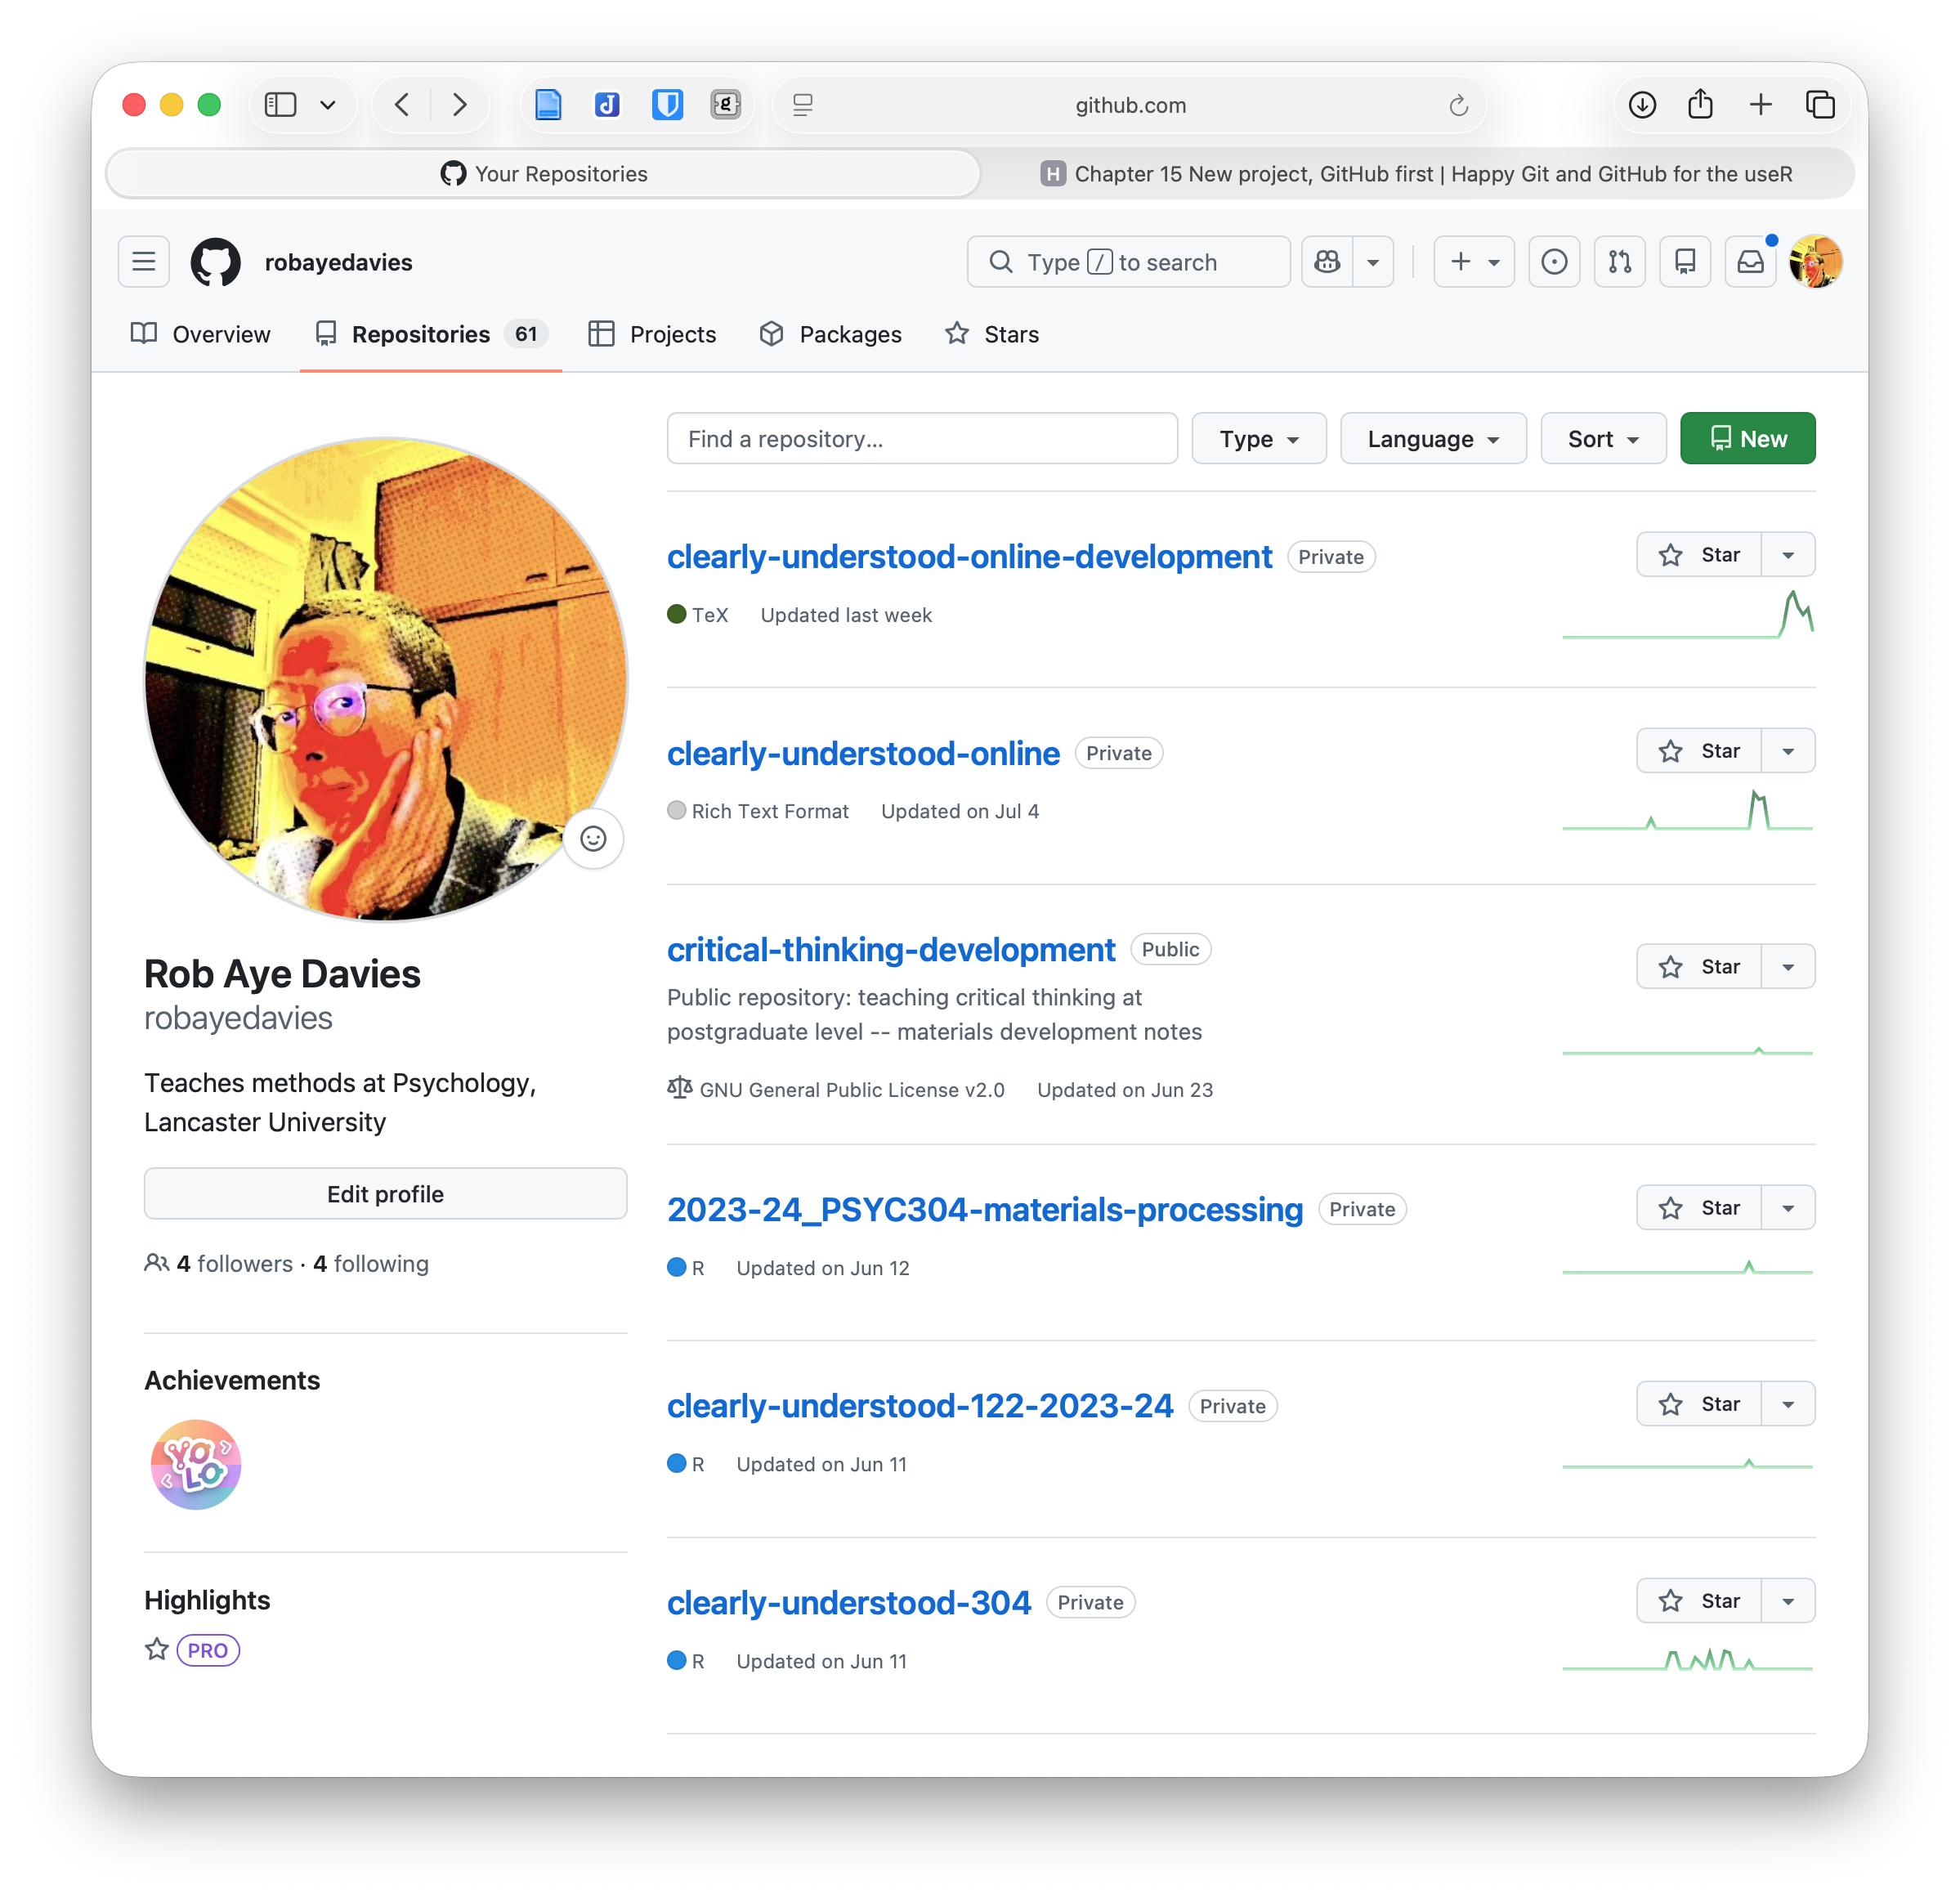
\includegraphics[width=0.6\linewidth,height=\textheight,keepaspectratio]{files/github-new-repo.png}

}

\caption{\label{fig-github-new-repo}GitHub new repo}

\end{figure}%

Near `Repositories', click the big green `New' button. Or, if you are on
your own profile page, click on `Repositories', then click the big green
`New' button.

\subsection{Name the repository, add a description, keep it public, add
a README, add .gitignore, add a
license}\label{name-the-repository-add-a-description-keep-it-public-add-a-readme-add-.gitignore-add-a-license}

\begin{figure}

\centering{

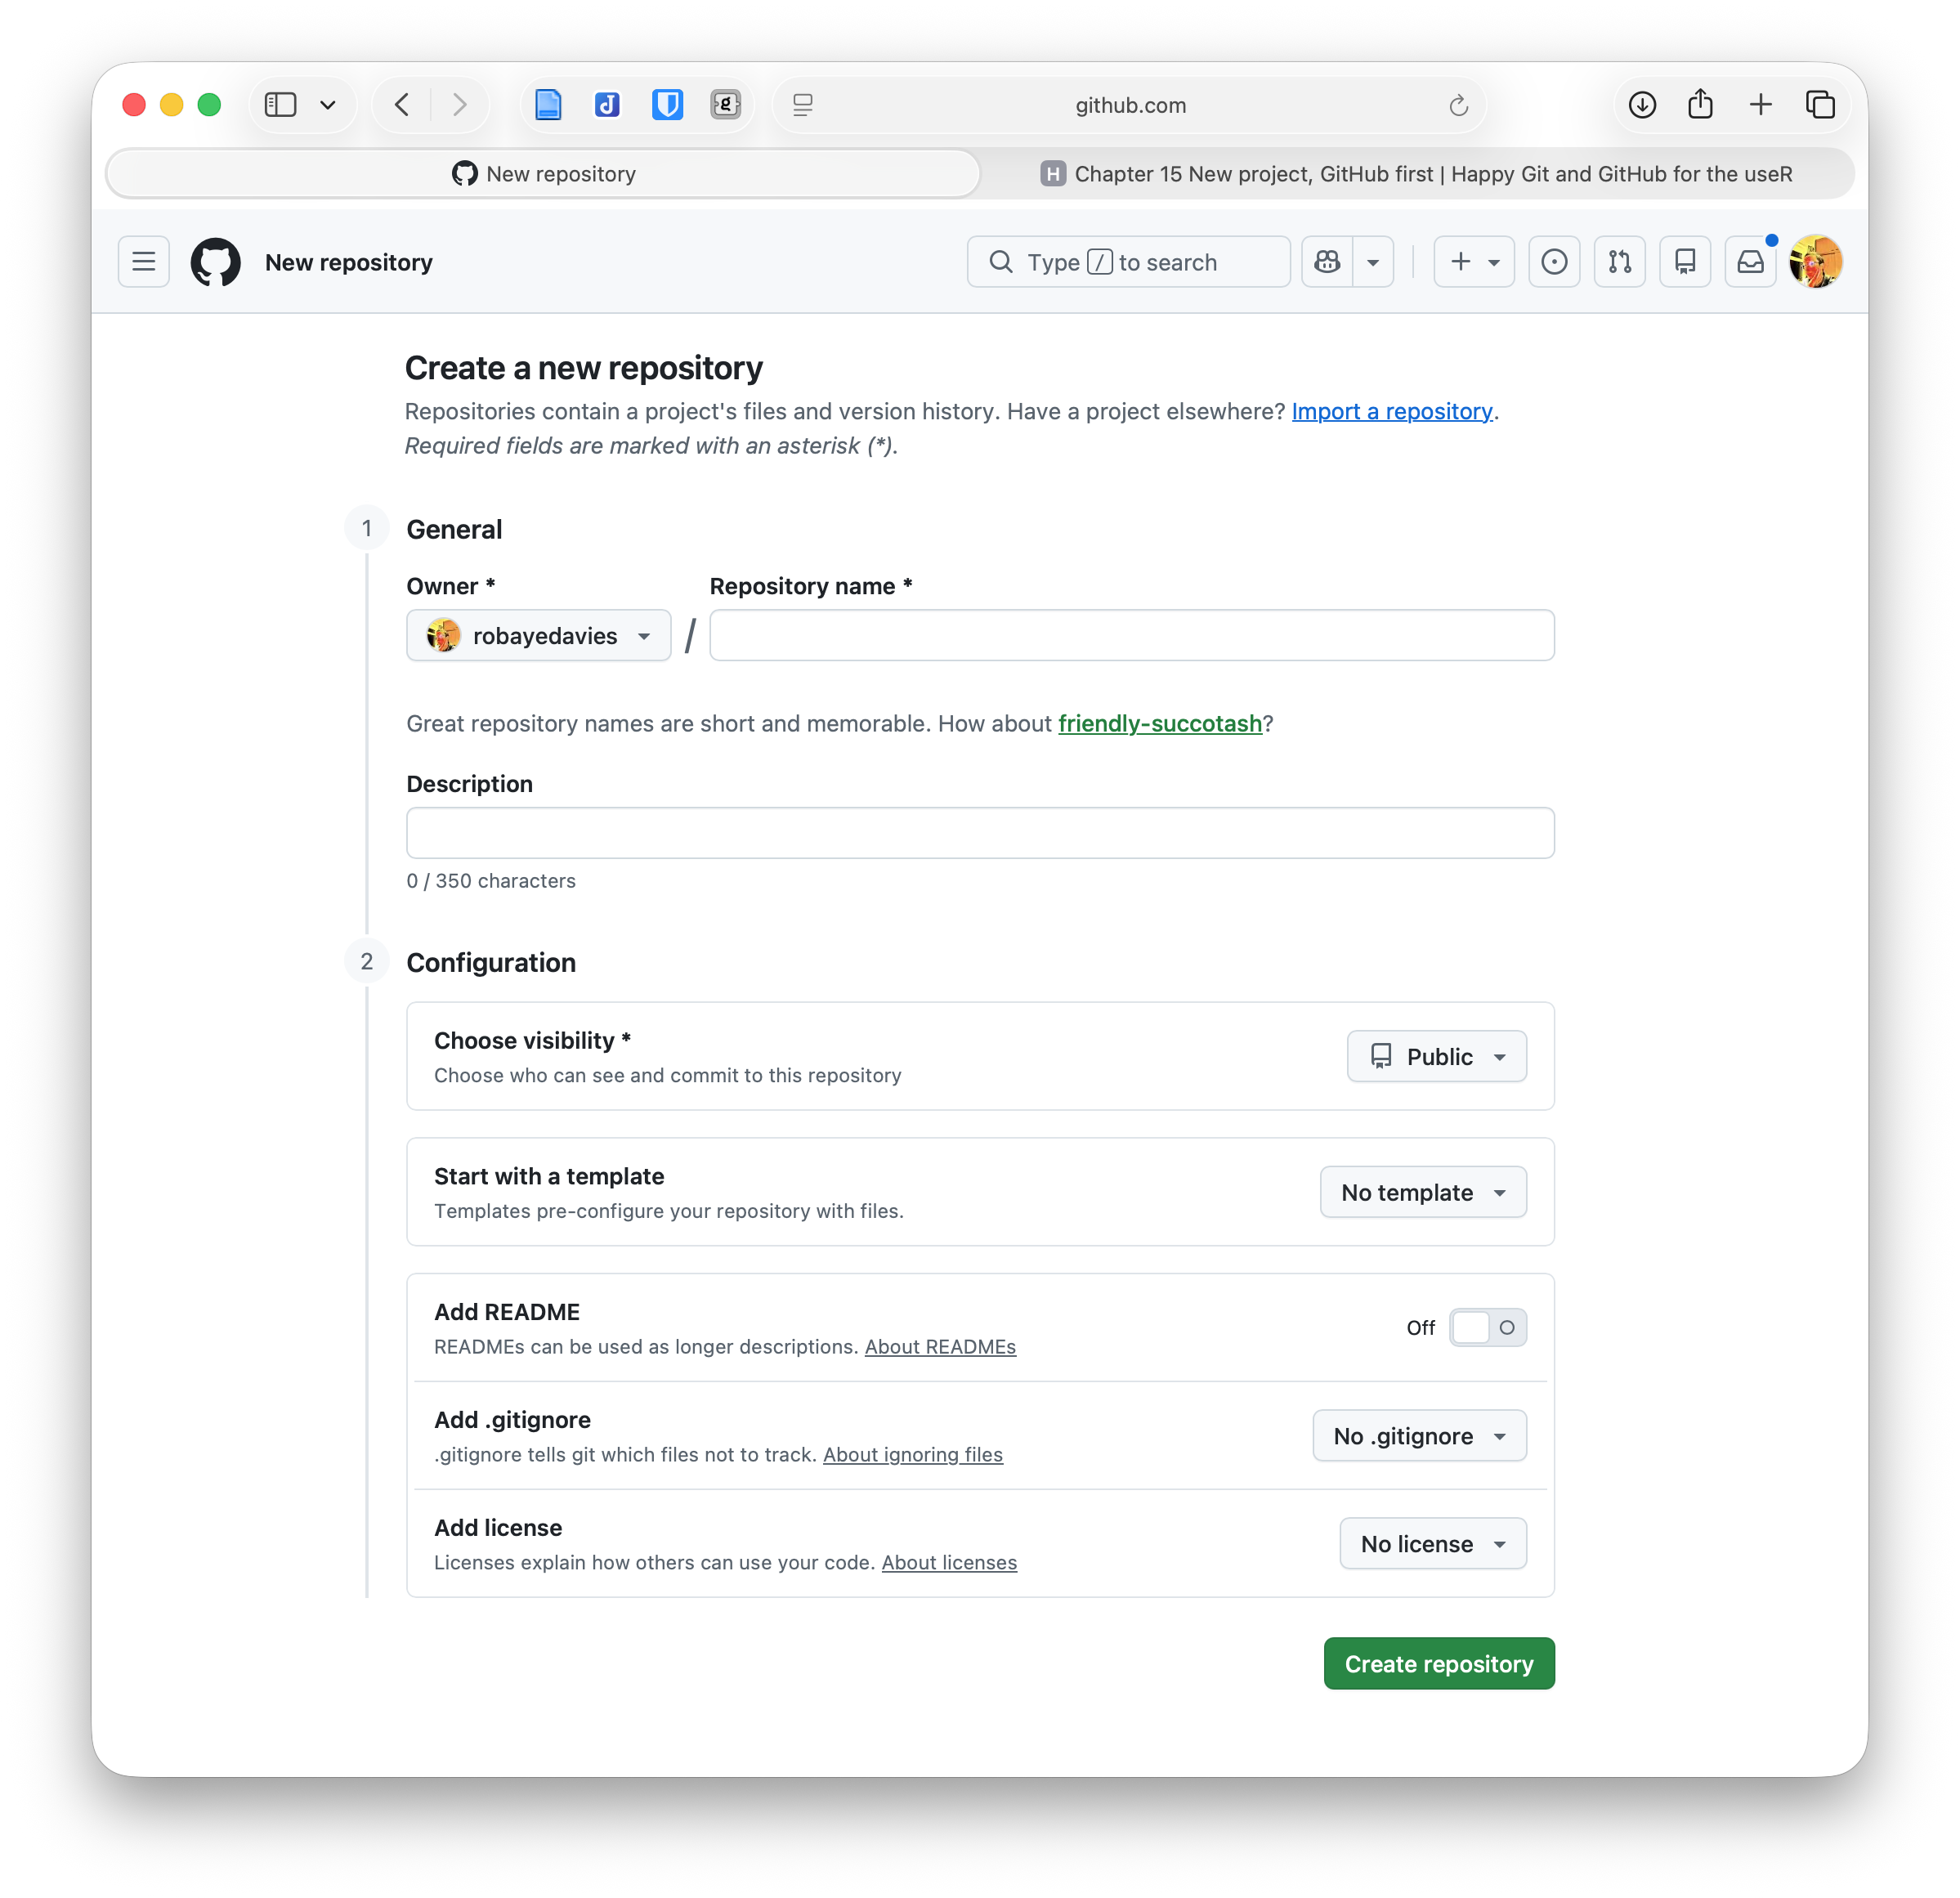
\includegraphics[width=0.6\linewidth,height=\textheight,keepaspectratio]{files/github-new-repo-name-public.png}

}

\caption{\label{fig-github-new-repo-name-public}github-new-repo-name-public}

\end{figure}%

You will have to enter some information:

\begin{itemize}
\tightlist
\item
  Repository template: No template.
\item
  Repository name: myrepo or whatever you wish to name your new project.
  Approach this similar to a variable name, in code: descriptive but
  brief, no whitespace. Letters, digits, \texttt{-}, \texttt{.}, or
  \texttt{\_} are allowed.
\item
  Description: any short description of the project.
\item
  Public.
\item
  Initialize this repository with: \texttt{Add\ a\ README\ file}.
\item
  Click the big green button that says \texttt{Create\ repository}.
\end{itemize}

\begin{figure}

\centering{

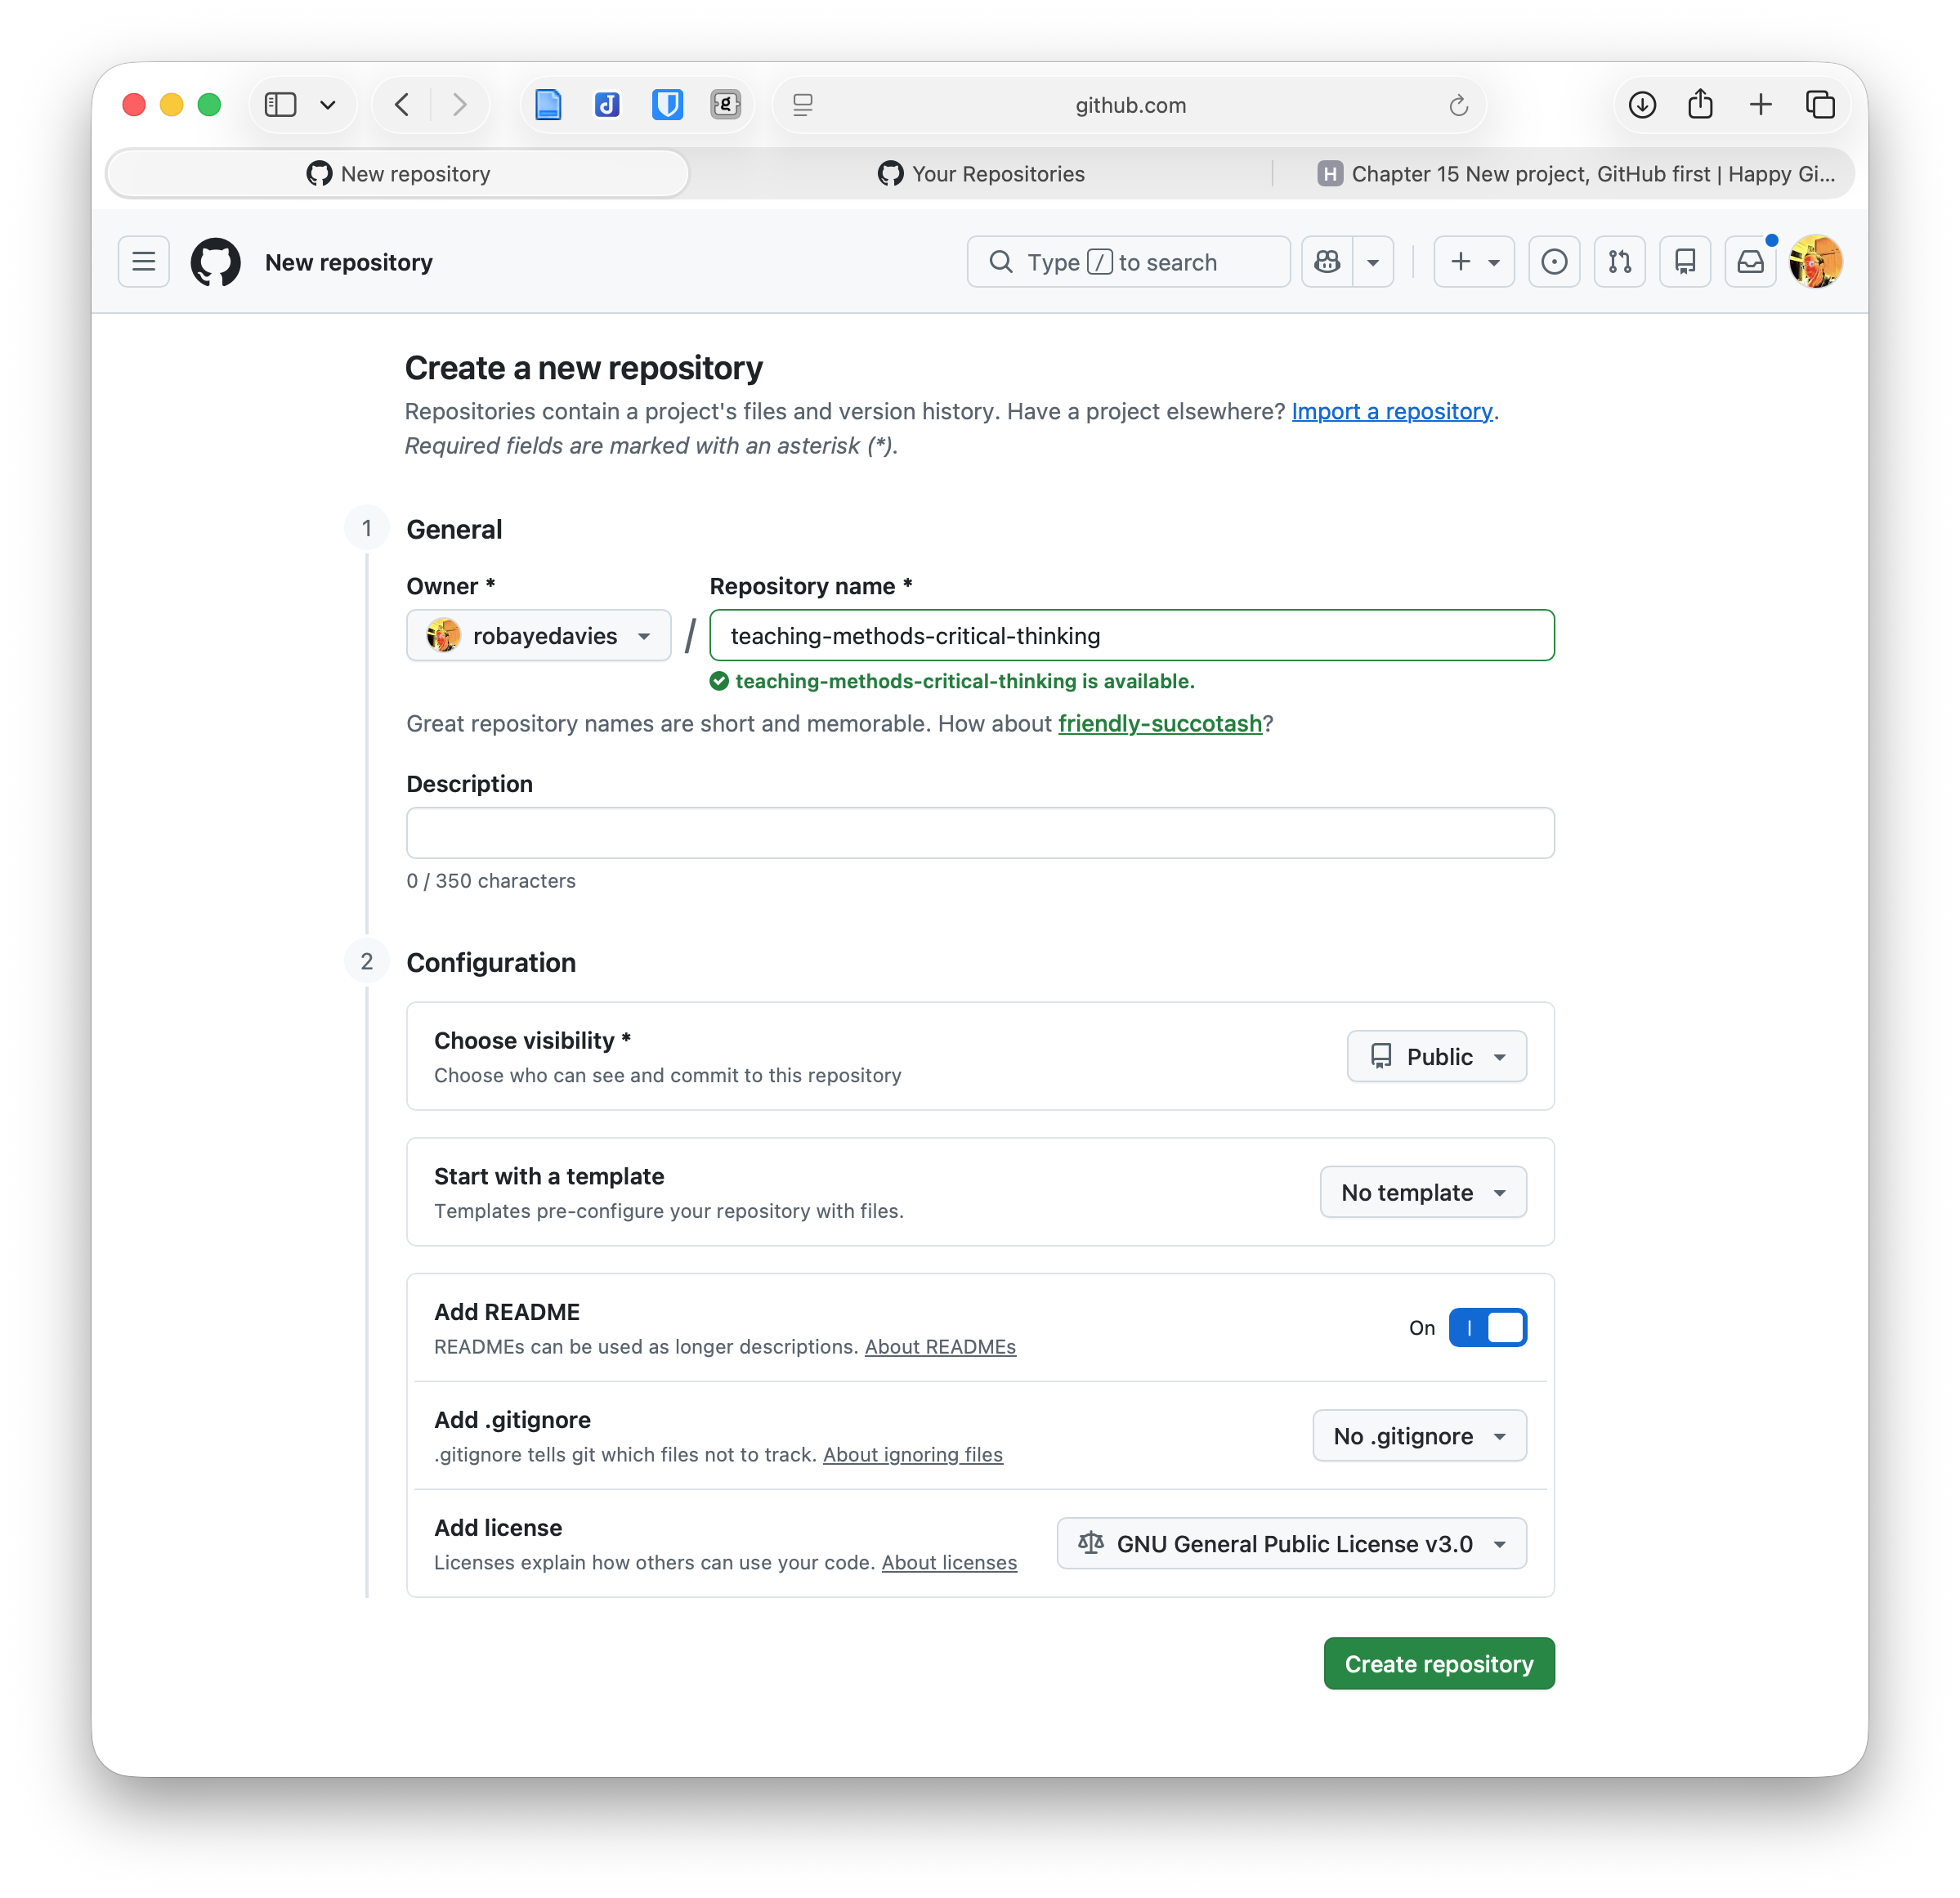
\includegraphics[width=0.6\linewidth,height=\textheight,keepaspectratio]{files/github-new-repo-name-public-values.png}

}

\caption{\label{fig-github-new-repo-name-public-values}github-new-repo-name-public-values}

\end{figure}%

Now click the big green button that says
\texttt{\textless{}\textgreater{}\ Code}. Copy a clone URL to your
clipboard. You will need this for the R-Studio side of the set-up.

\begin{figure}

\centering{

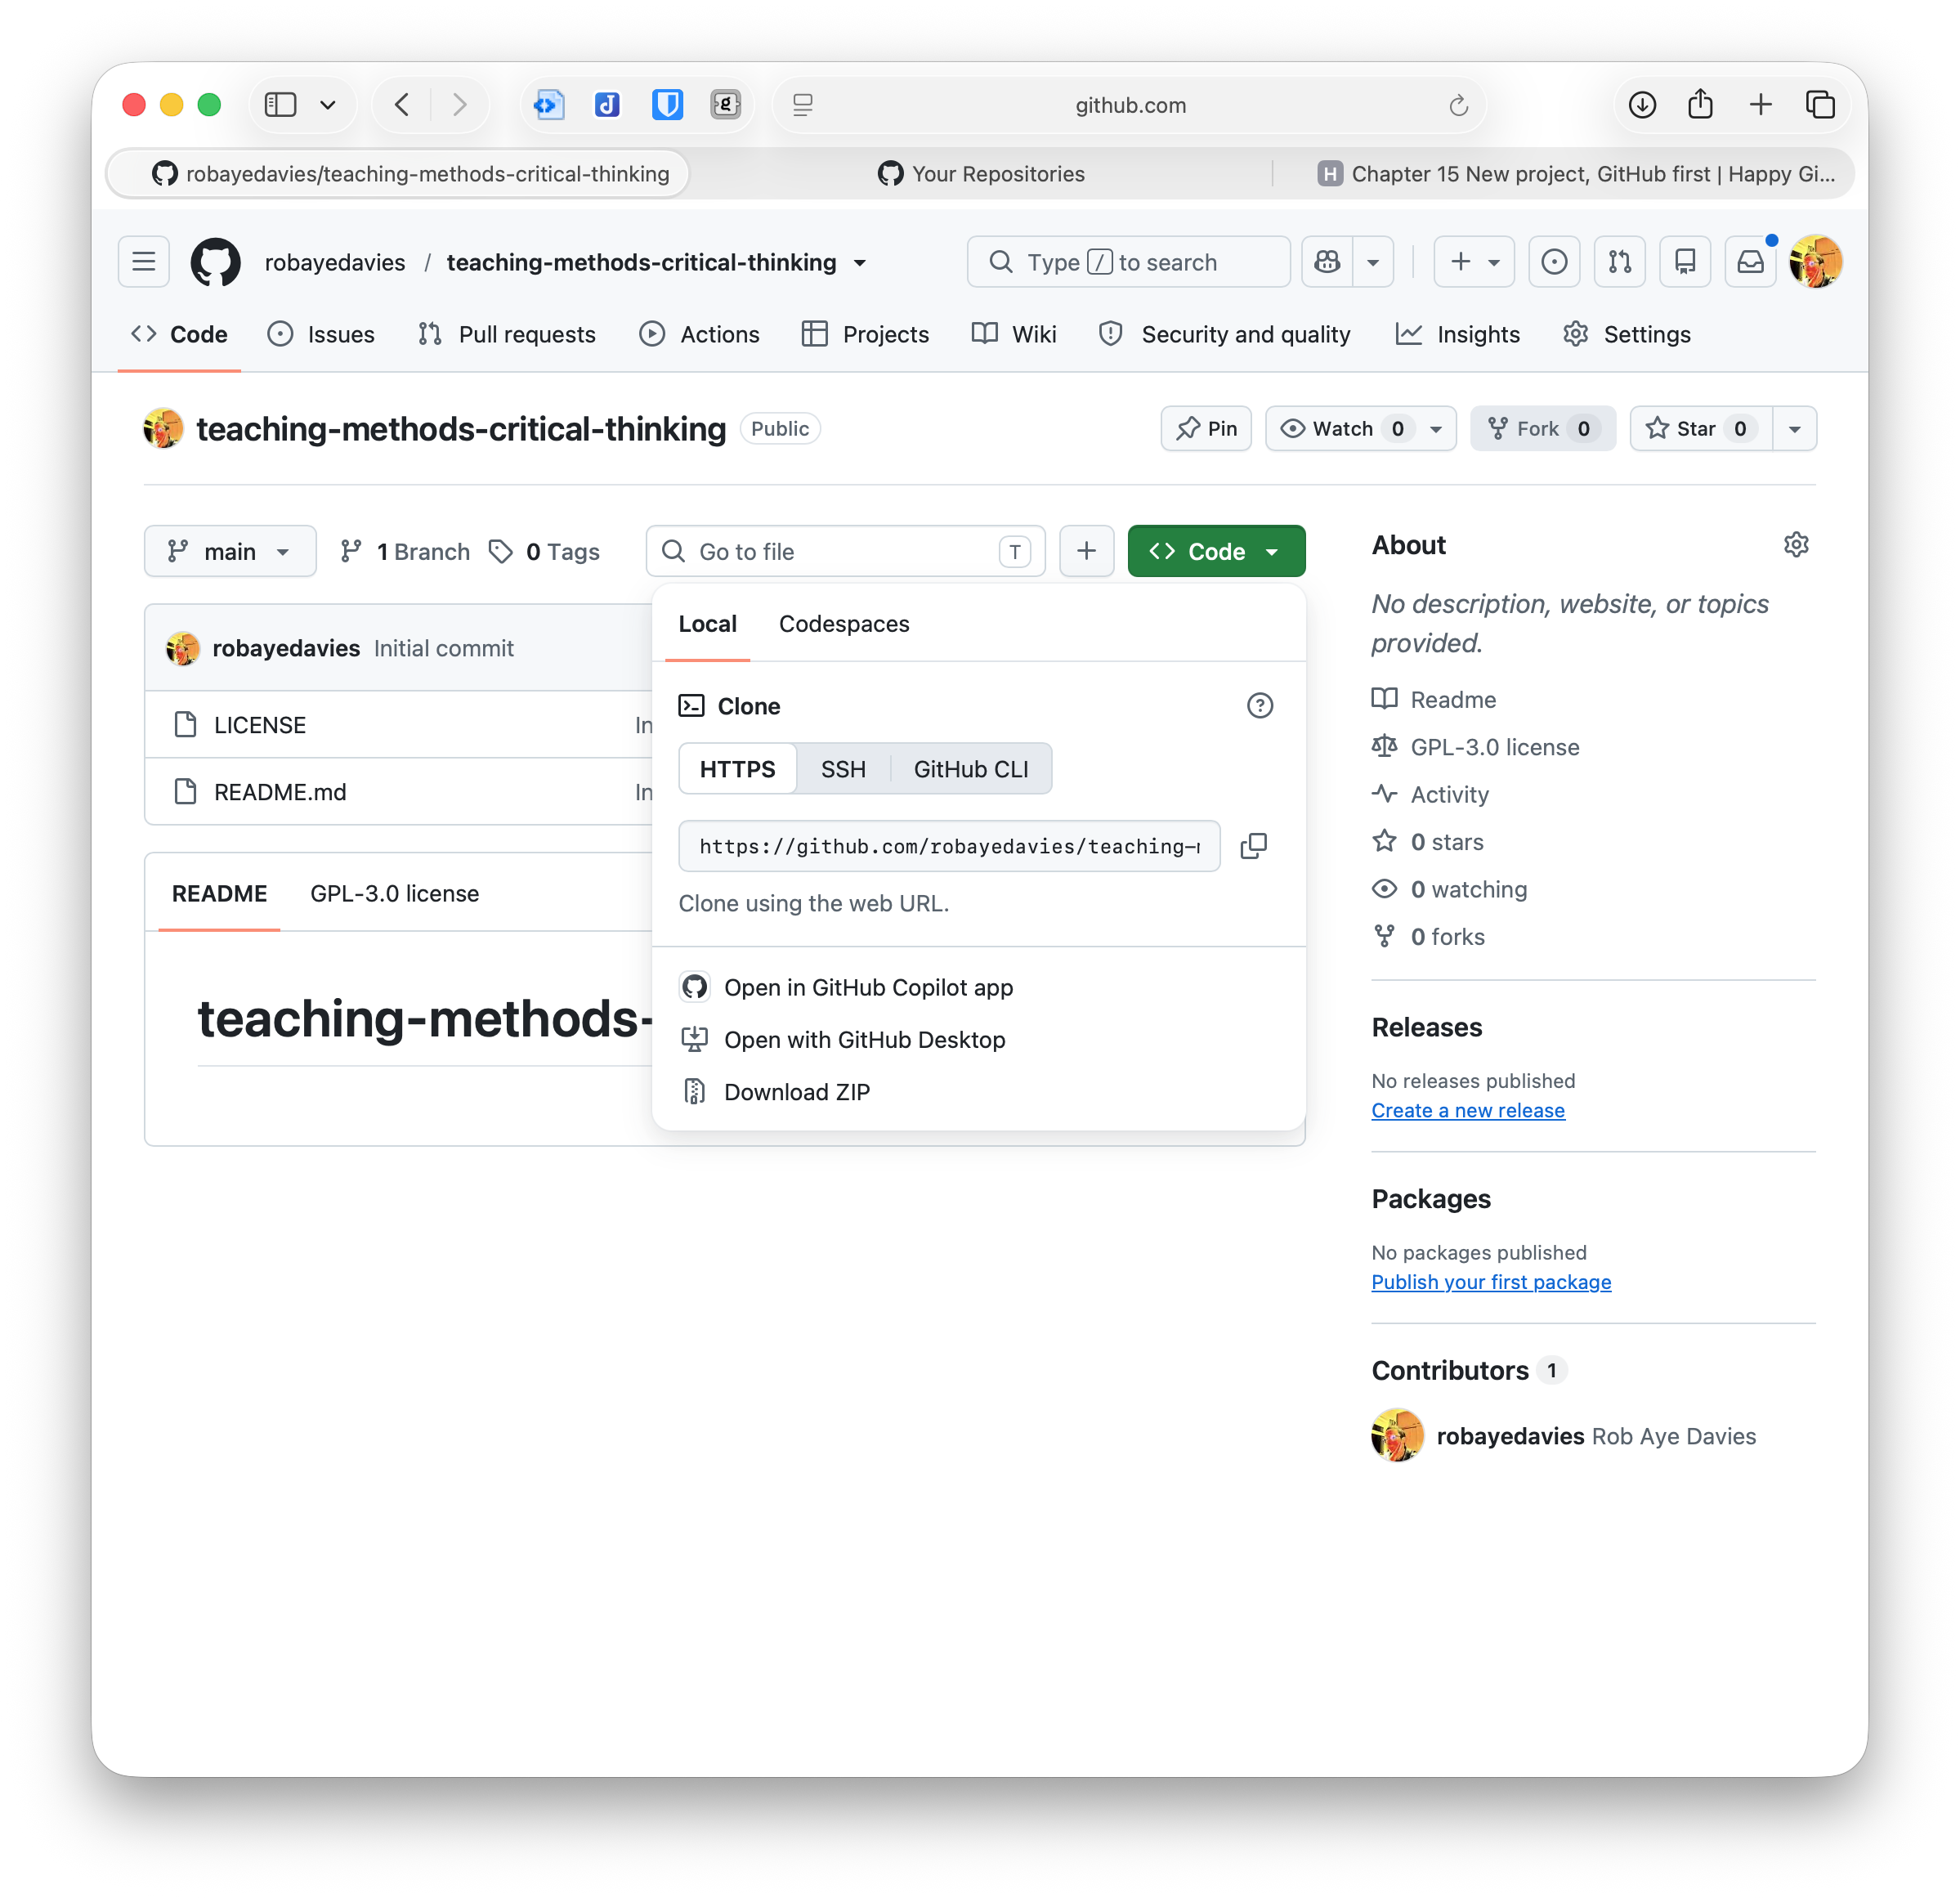
\includegraphics[width=0.6\linewidth,height=\textheight,keepaspectratio]{files/github-new-repo-url.png}

}

\caption{\label{fig-github-new-repo-url}github-new-repo-url}

\end{figure}%

\subsection{Now, in RStudio, set up a project (GitHub repo
first)}\label{now-in-rstudio-set-up-a-project-github-repo-first}

We are going to create a project, using version control.

File \textgreater{} New Project \textgreater{} Version control

\begin{figure}

\centering{

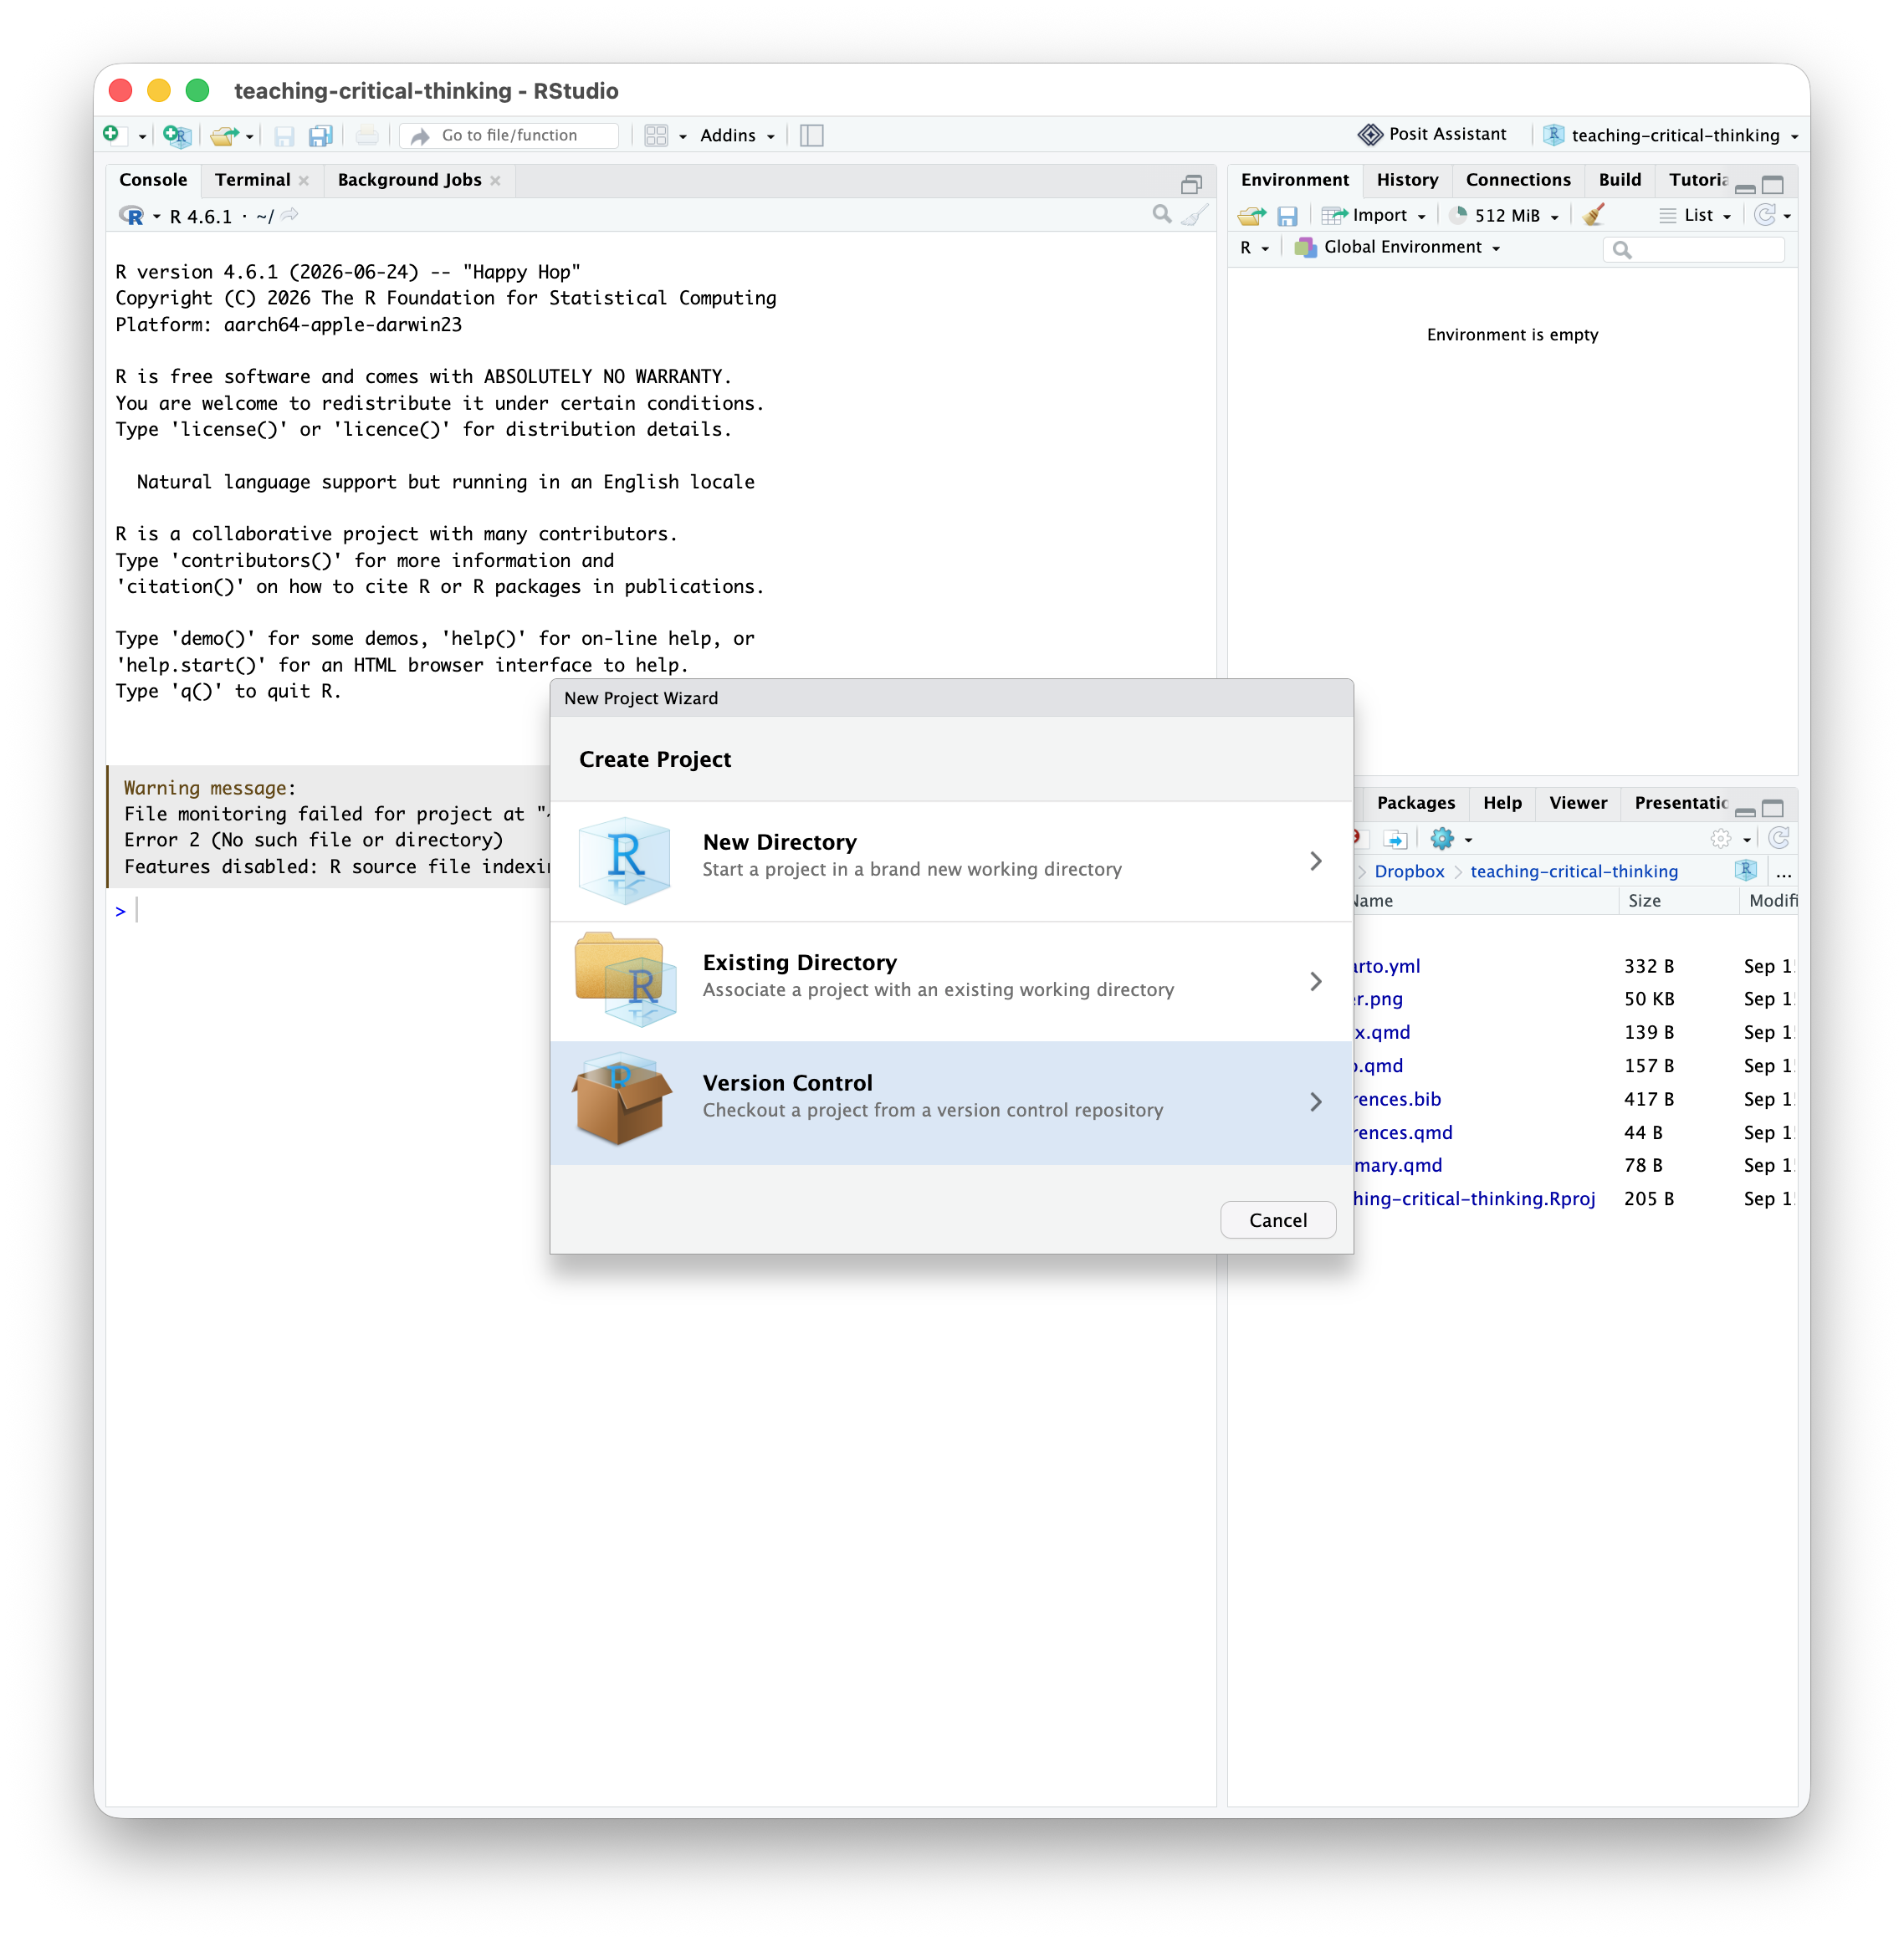
\includegraphics[width=0.6\linewidth,height=\textheight,keepaspectratio]{files/rstudio-create-project-version-control.png}

}

\caption{\label{fig-rstudio-create-project-version-control}rstudio-create-project-version-control}

\end{figure}%

We will be cloning a project from a Git repository: the repo we just
created.

File \textgreater{} New Project \textgreater{} Version control
\textgreater{} Git

\begin{figure}

\centering{

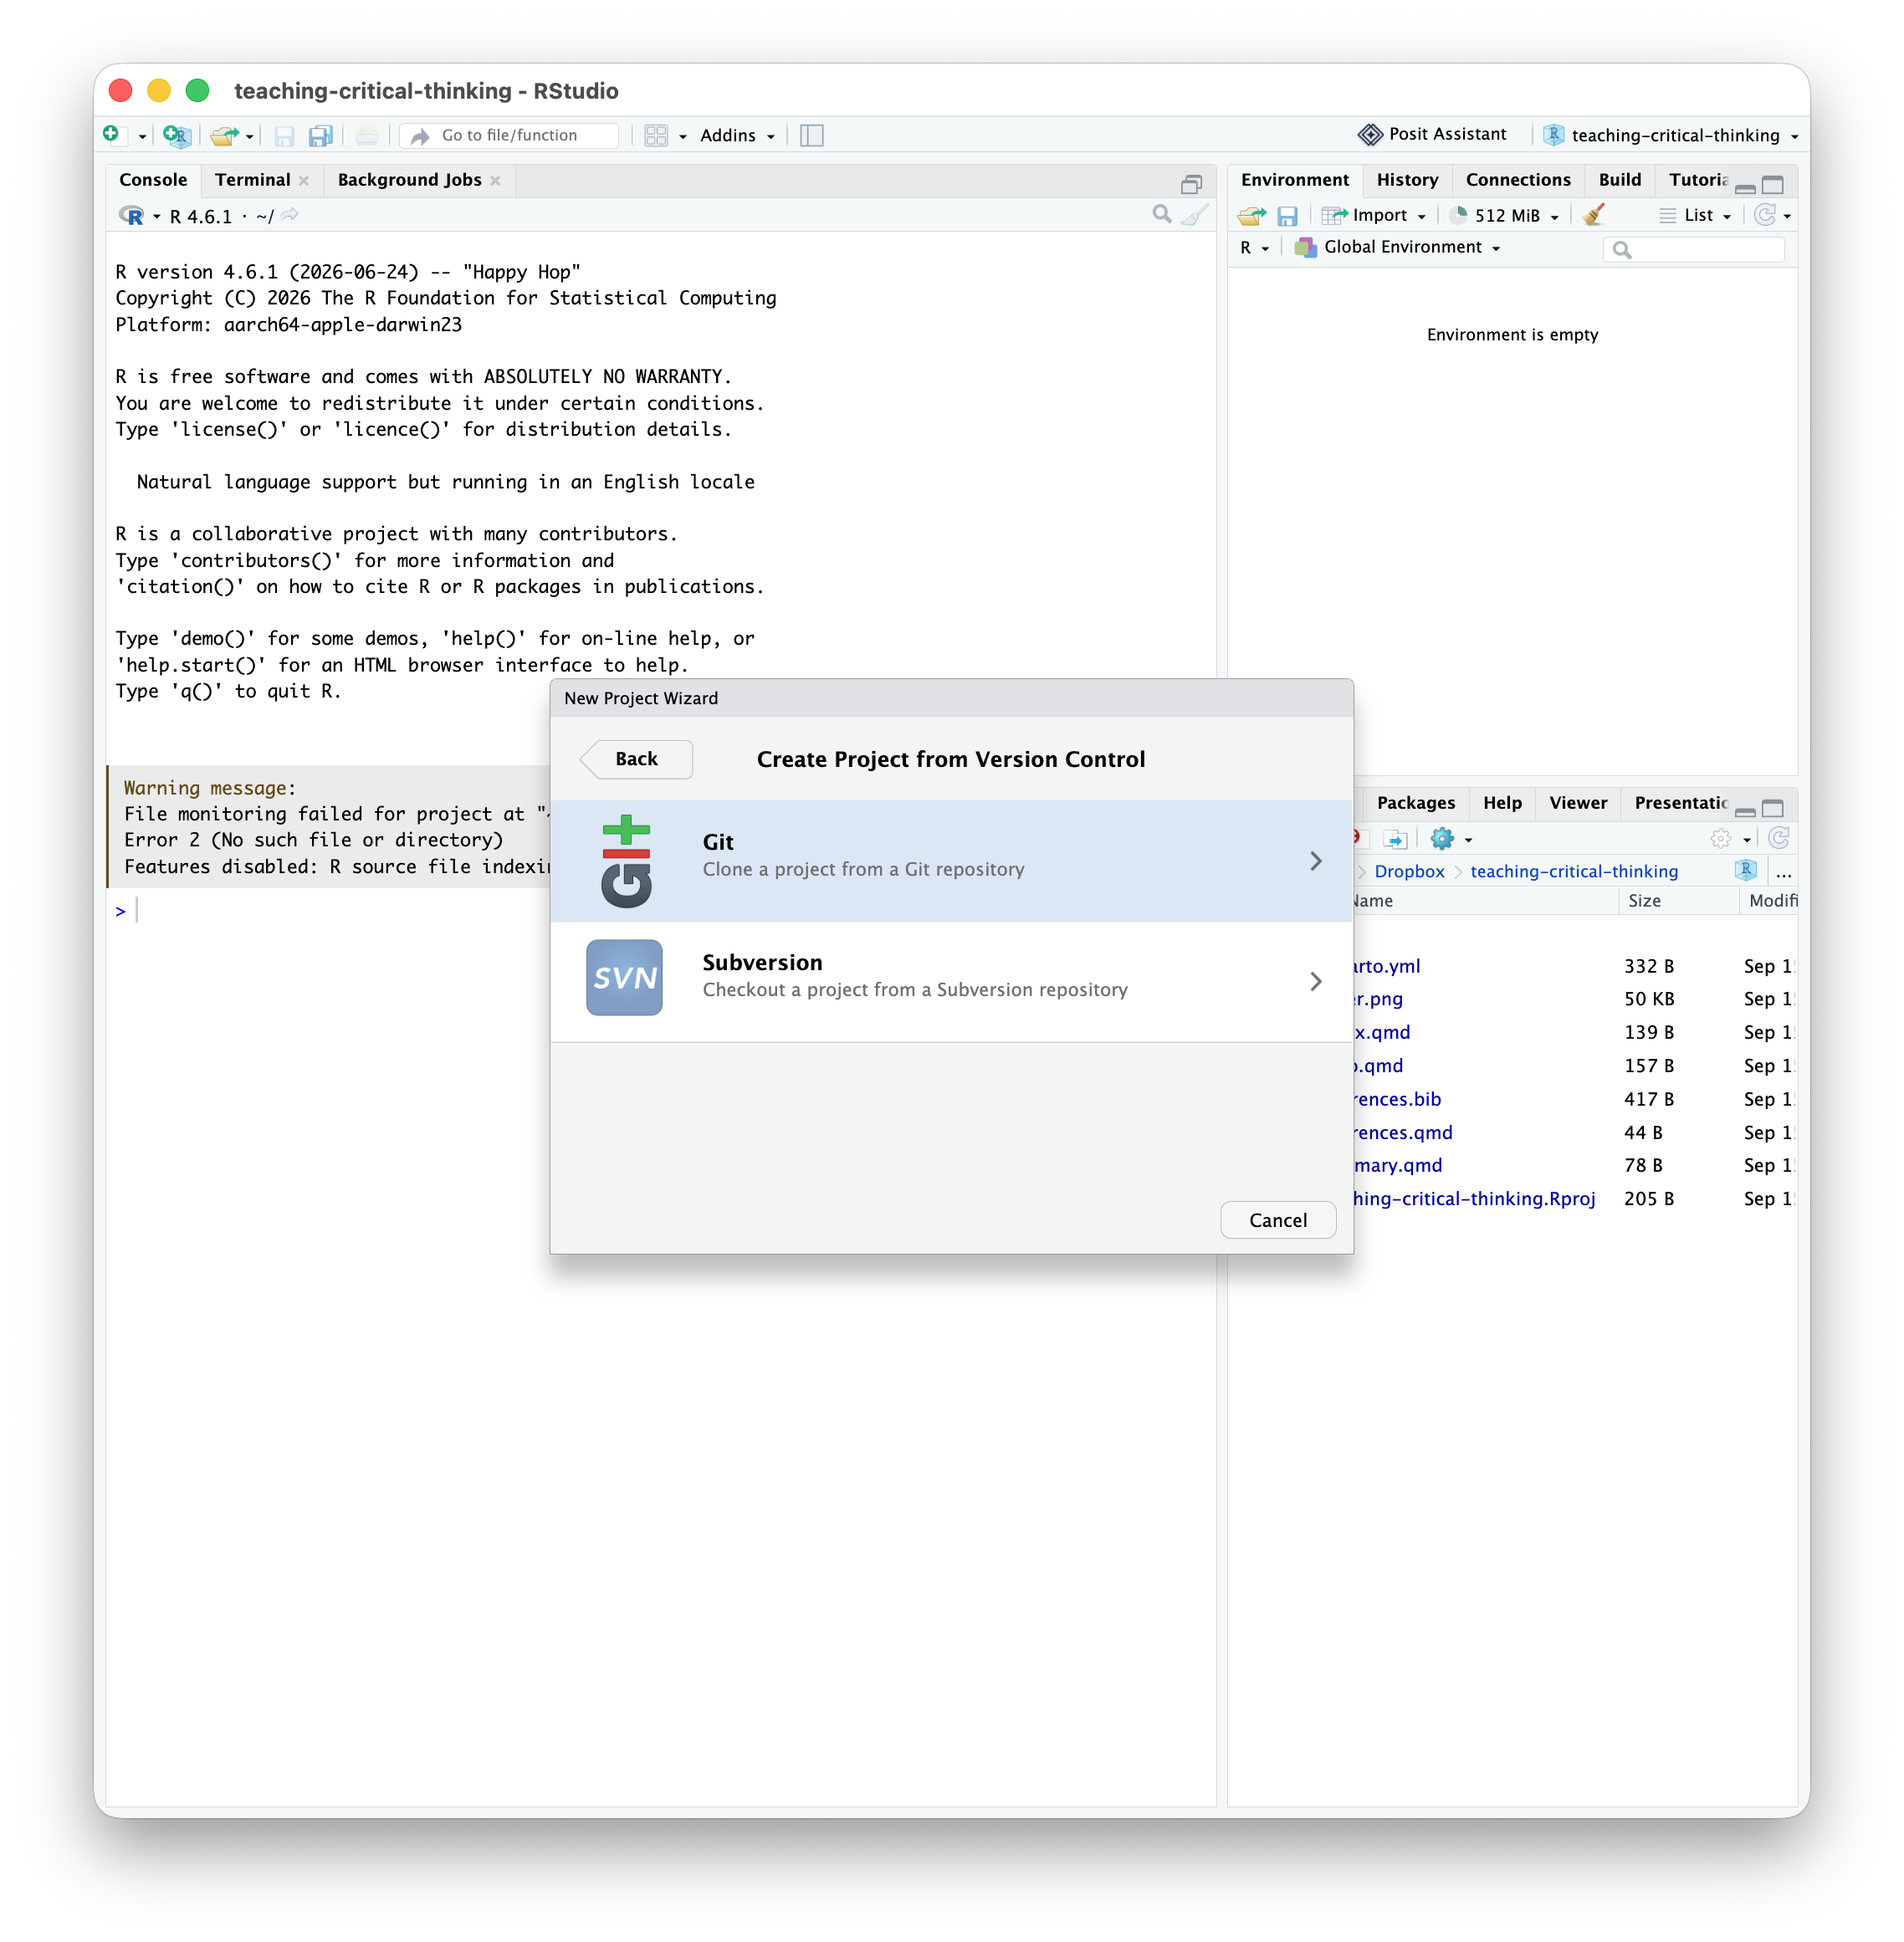
\includegraphics[width=0.6\linewidth,height=\textheight,keepaspectratio]{files/rstudio-create-project-version-control-git.png}

}

\caption{\label{fig-rstudio-create-project-version-control-git}rstudio-create-project-version-control-git}

\end{figure}%

Enter the URL from the GitHub repository.

\begin{itemize}
\tightlist
\item
  Remember where we got the URL:
\end{itemize}

\begin{figure}

\centering{

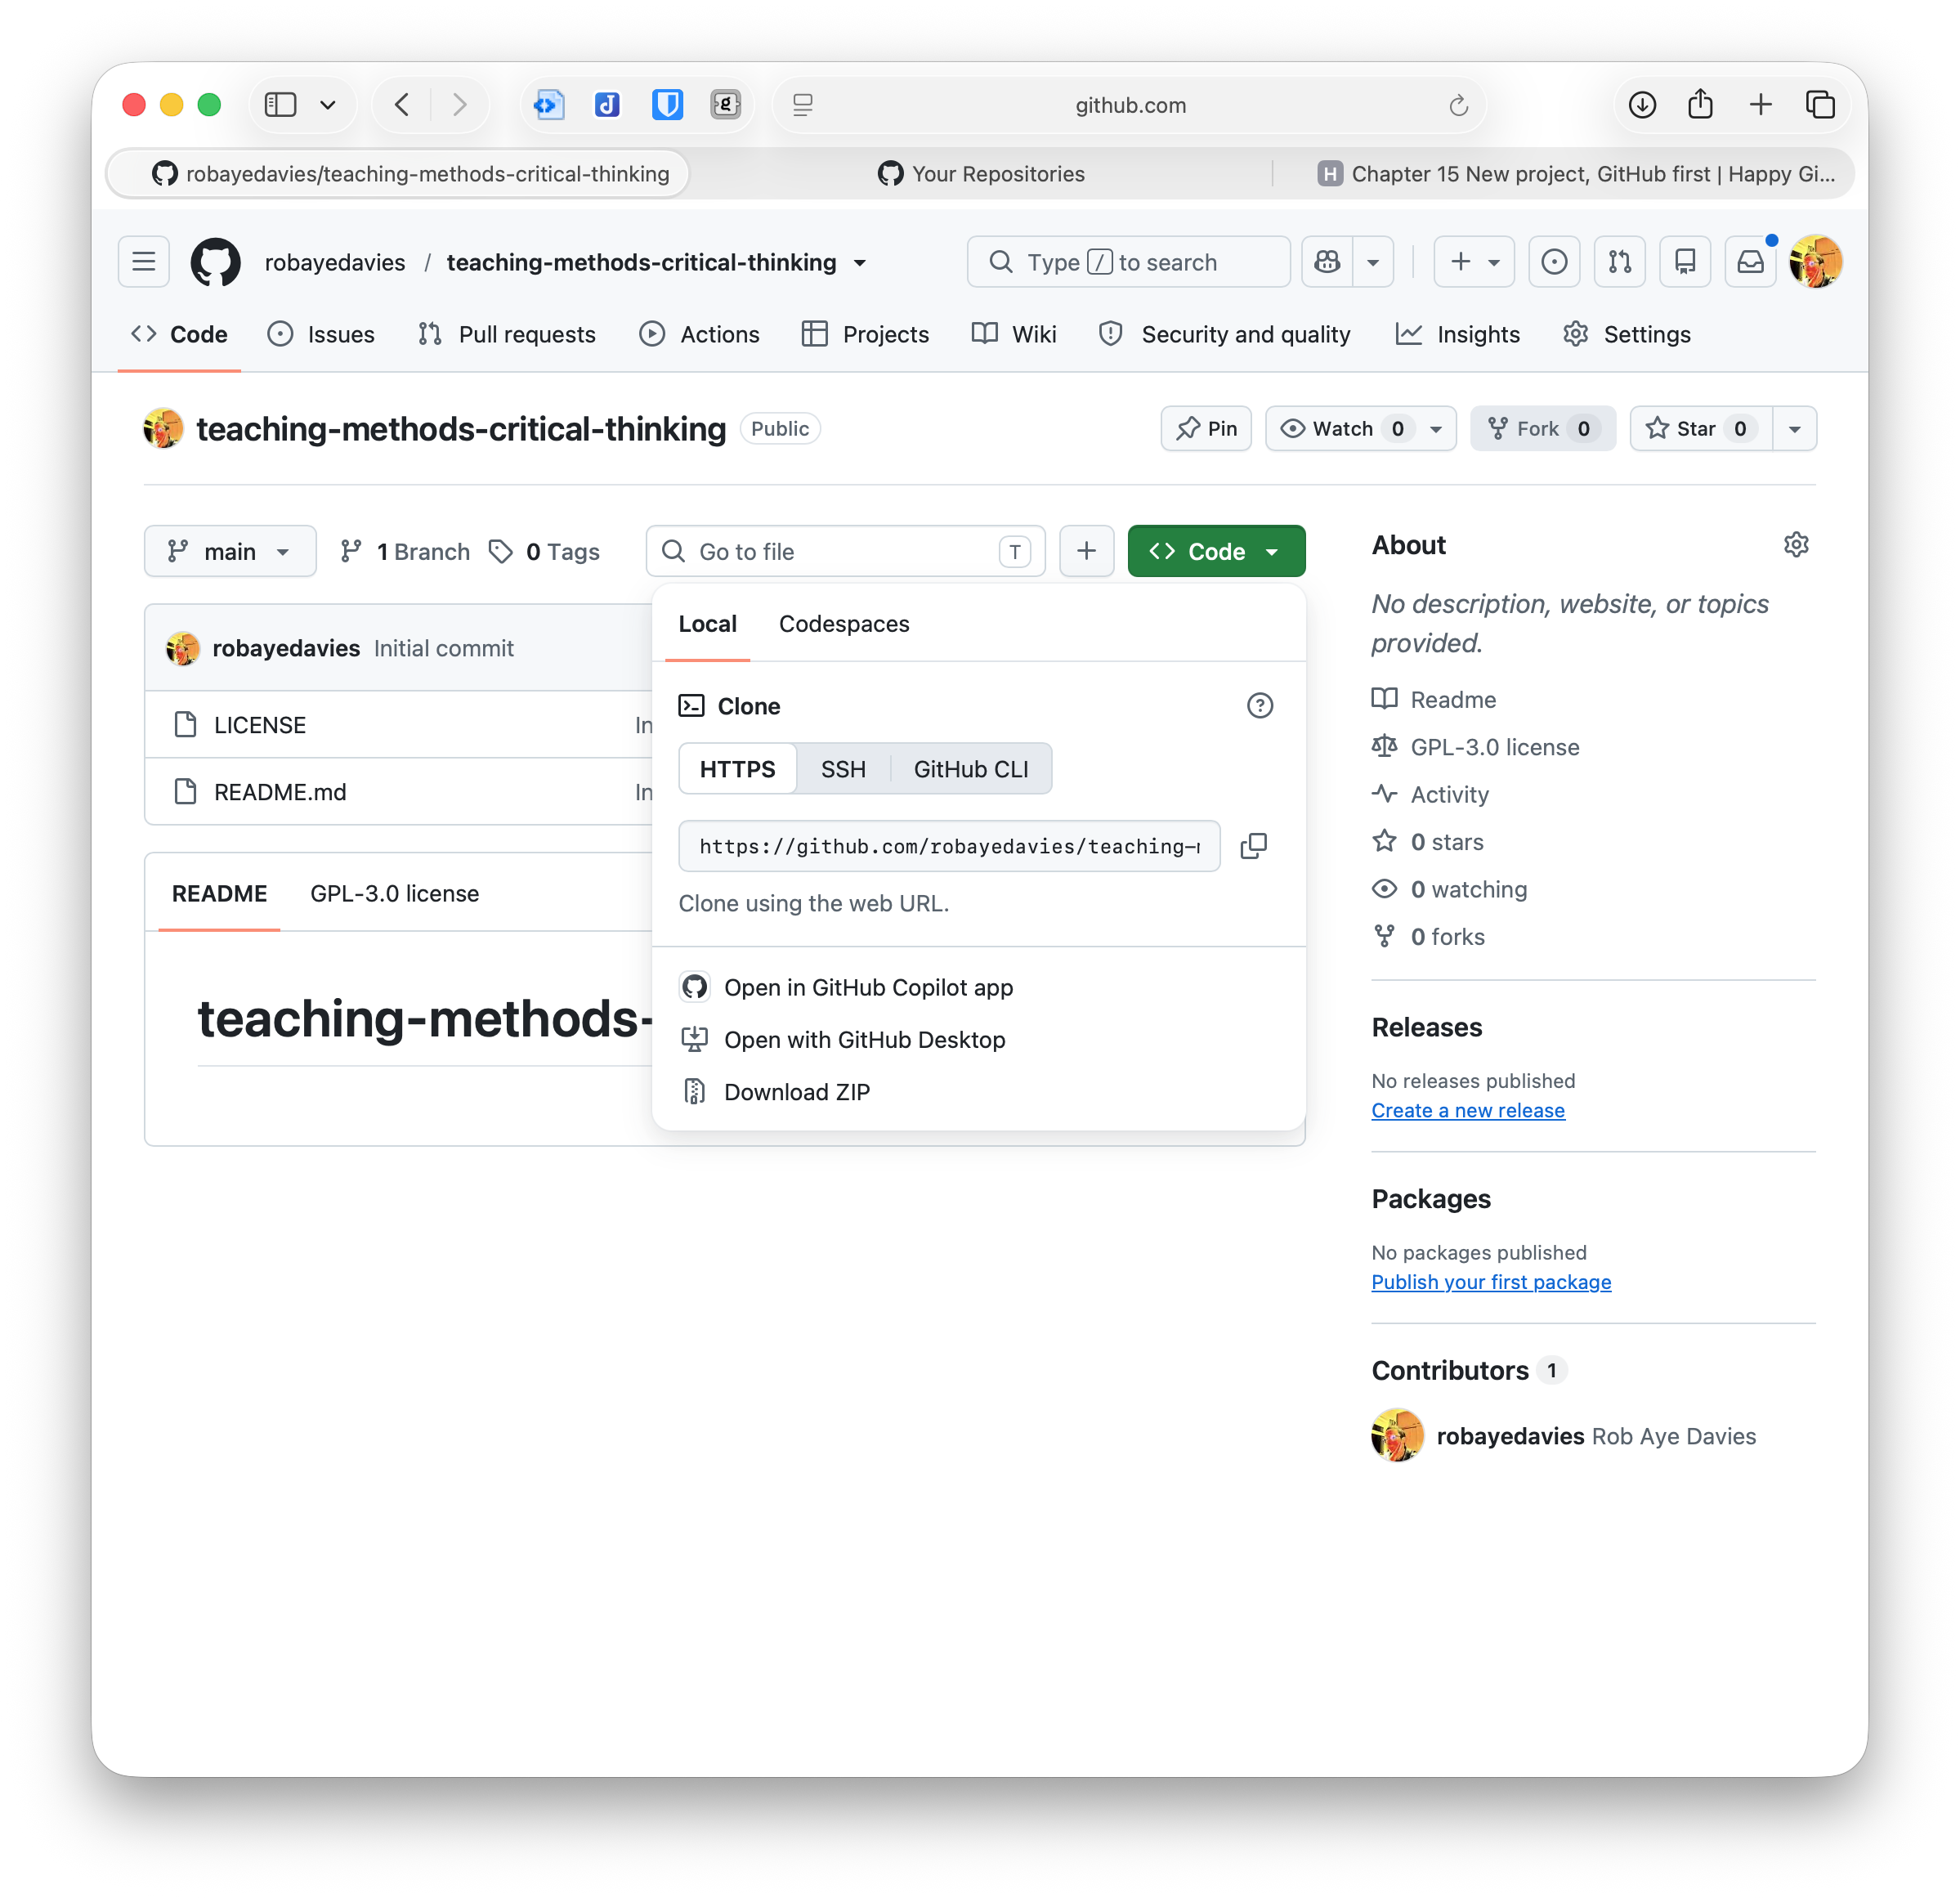
\includegraphics[width=0.6\linewidth,height=\textheight,keepaspectratio]{files/github-new-repo-url.png}

}

\caption{\label{fig-github-new-repo-url}github-new-repo-url}

\end{figure}%

In RStudio, enter the URL in the \texttt{Clone\ Git\ Repository}
dialogue box.

\begin{figure}

\centering{

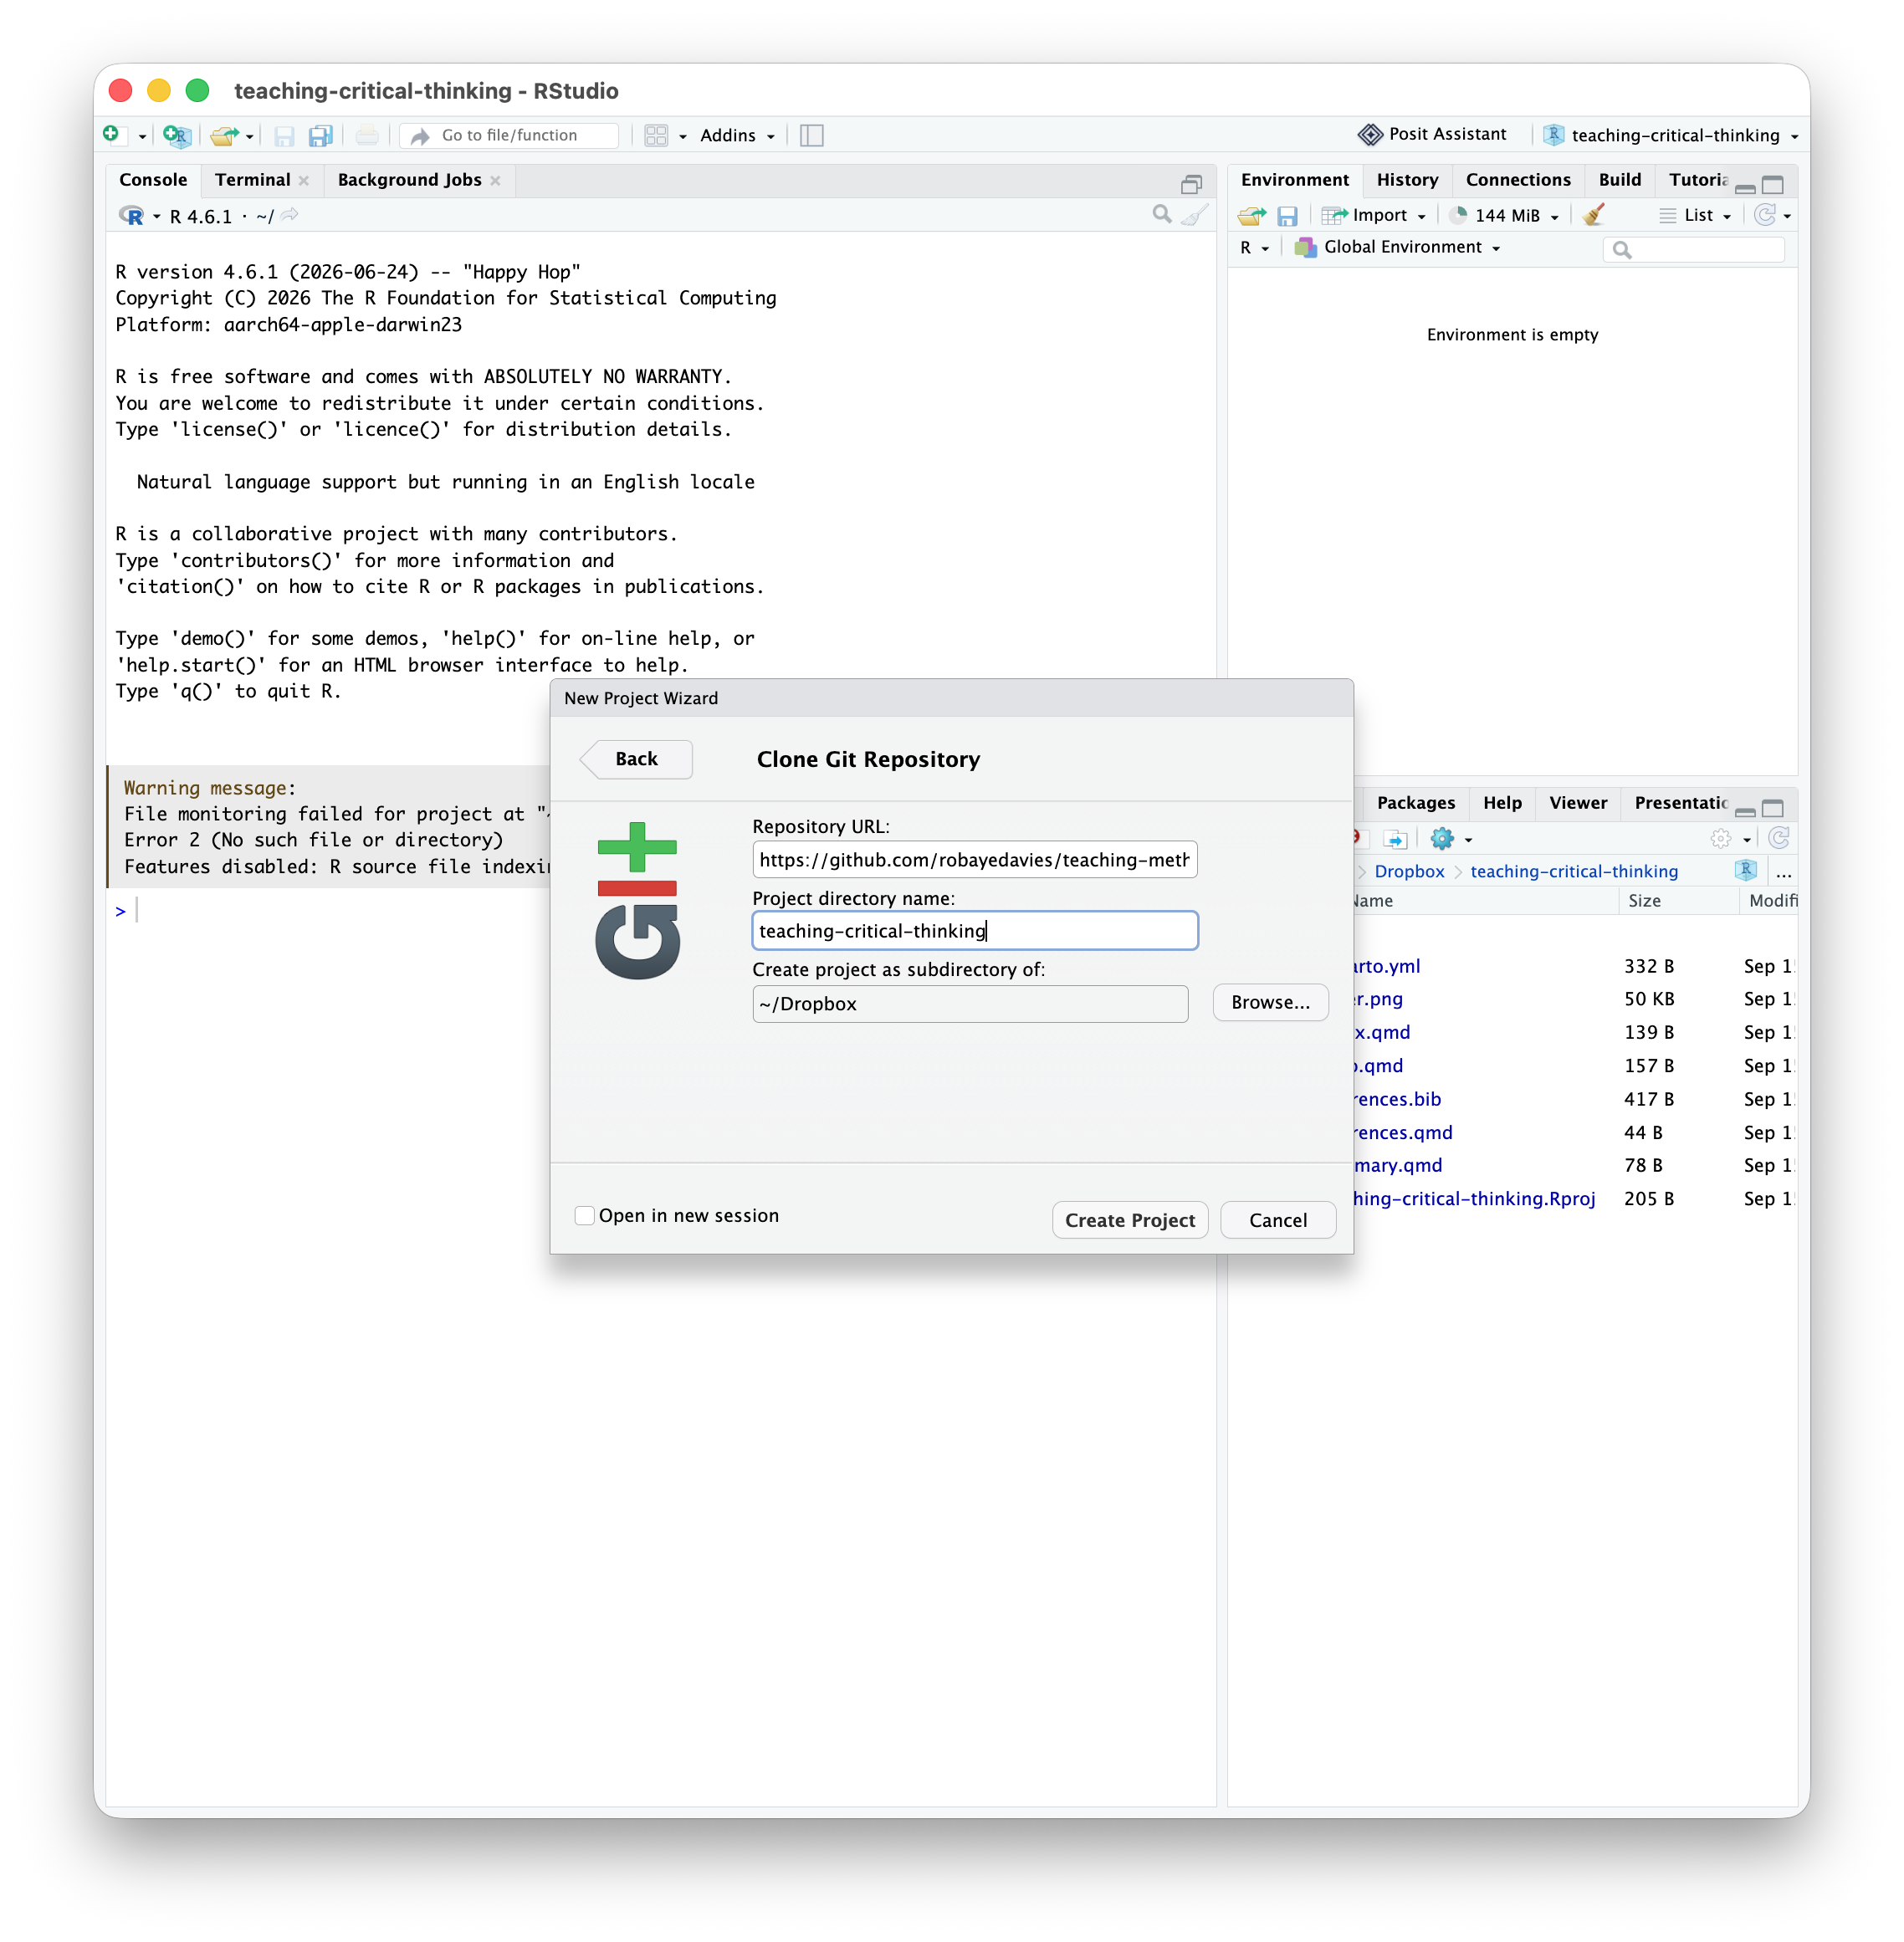
\includegraphics[width=0.6\linewidth,height=\textheight,keepaspectratio]{files/rstudio-create-project-version-control-git-url.png}

}

\caption{\label{fig-rstudio-create-project-version-control-git-url}rstudio-create-project-version-control-git-url}

\end{figure}%

Click on \textbf{\texttt{Create\ Project}}.

The project folder (and all its contents) is now on your local hard
drive.

\begin{figure}

\centering{

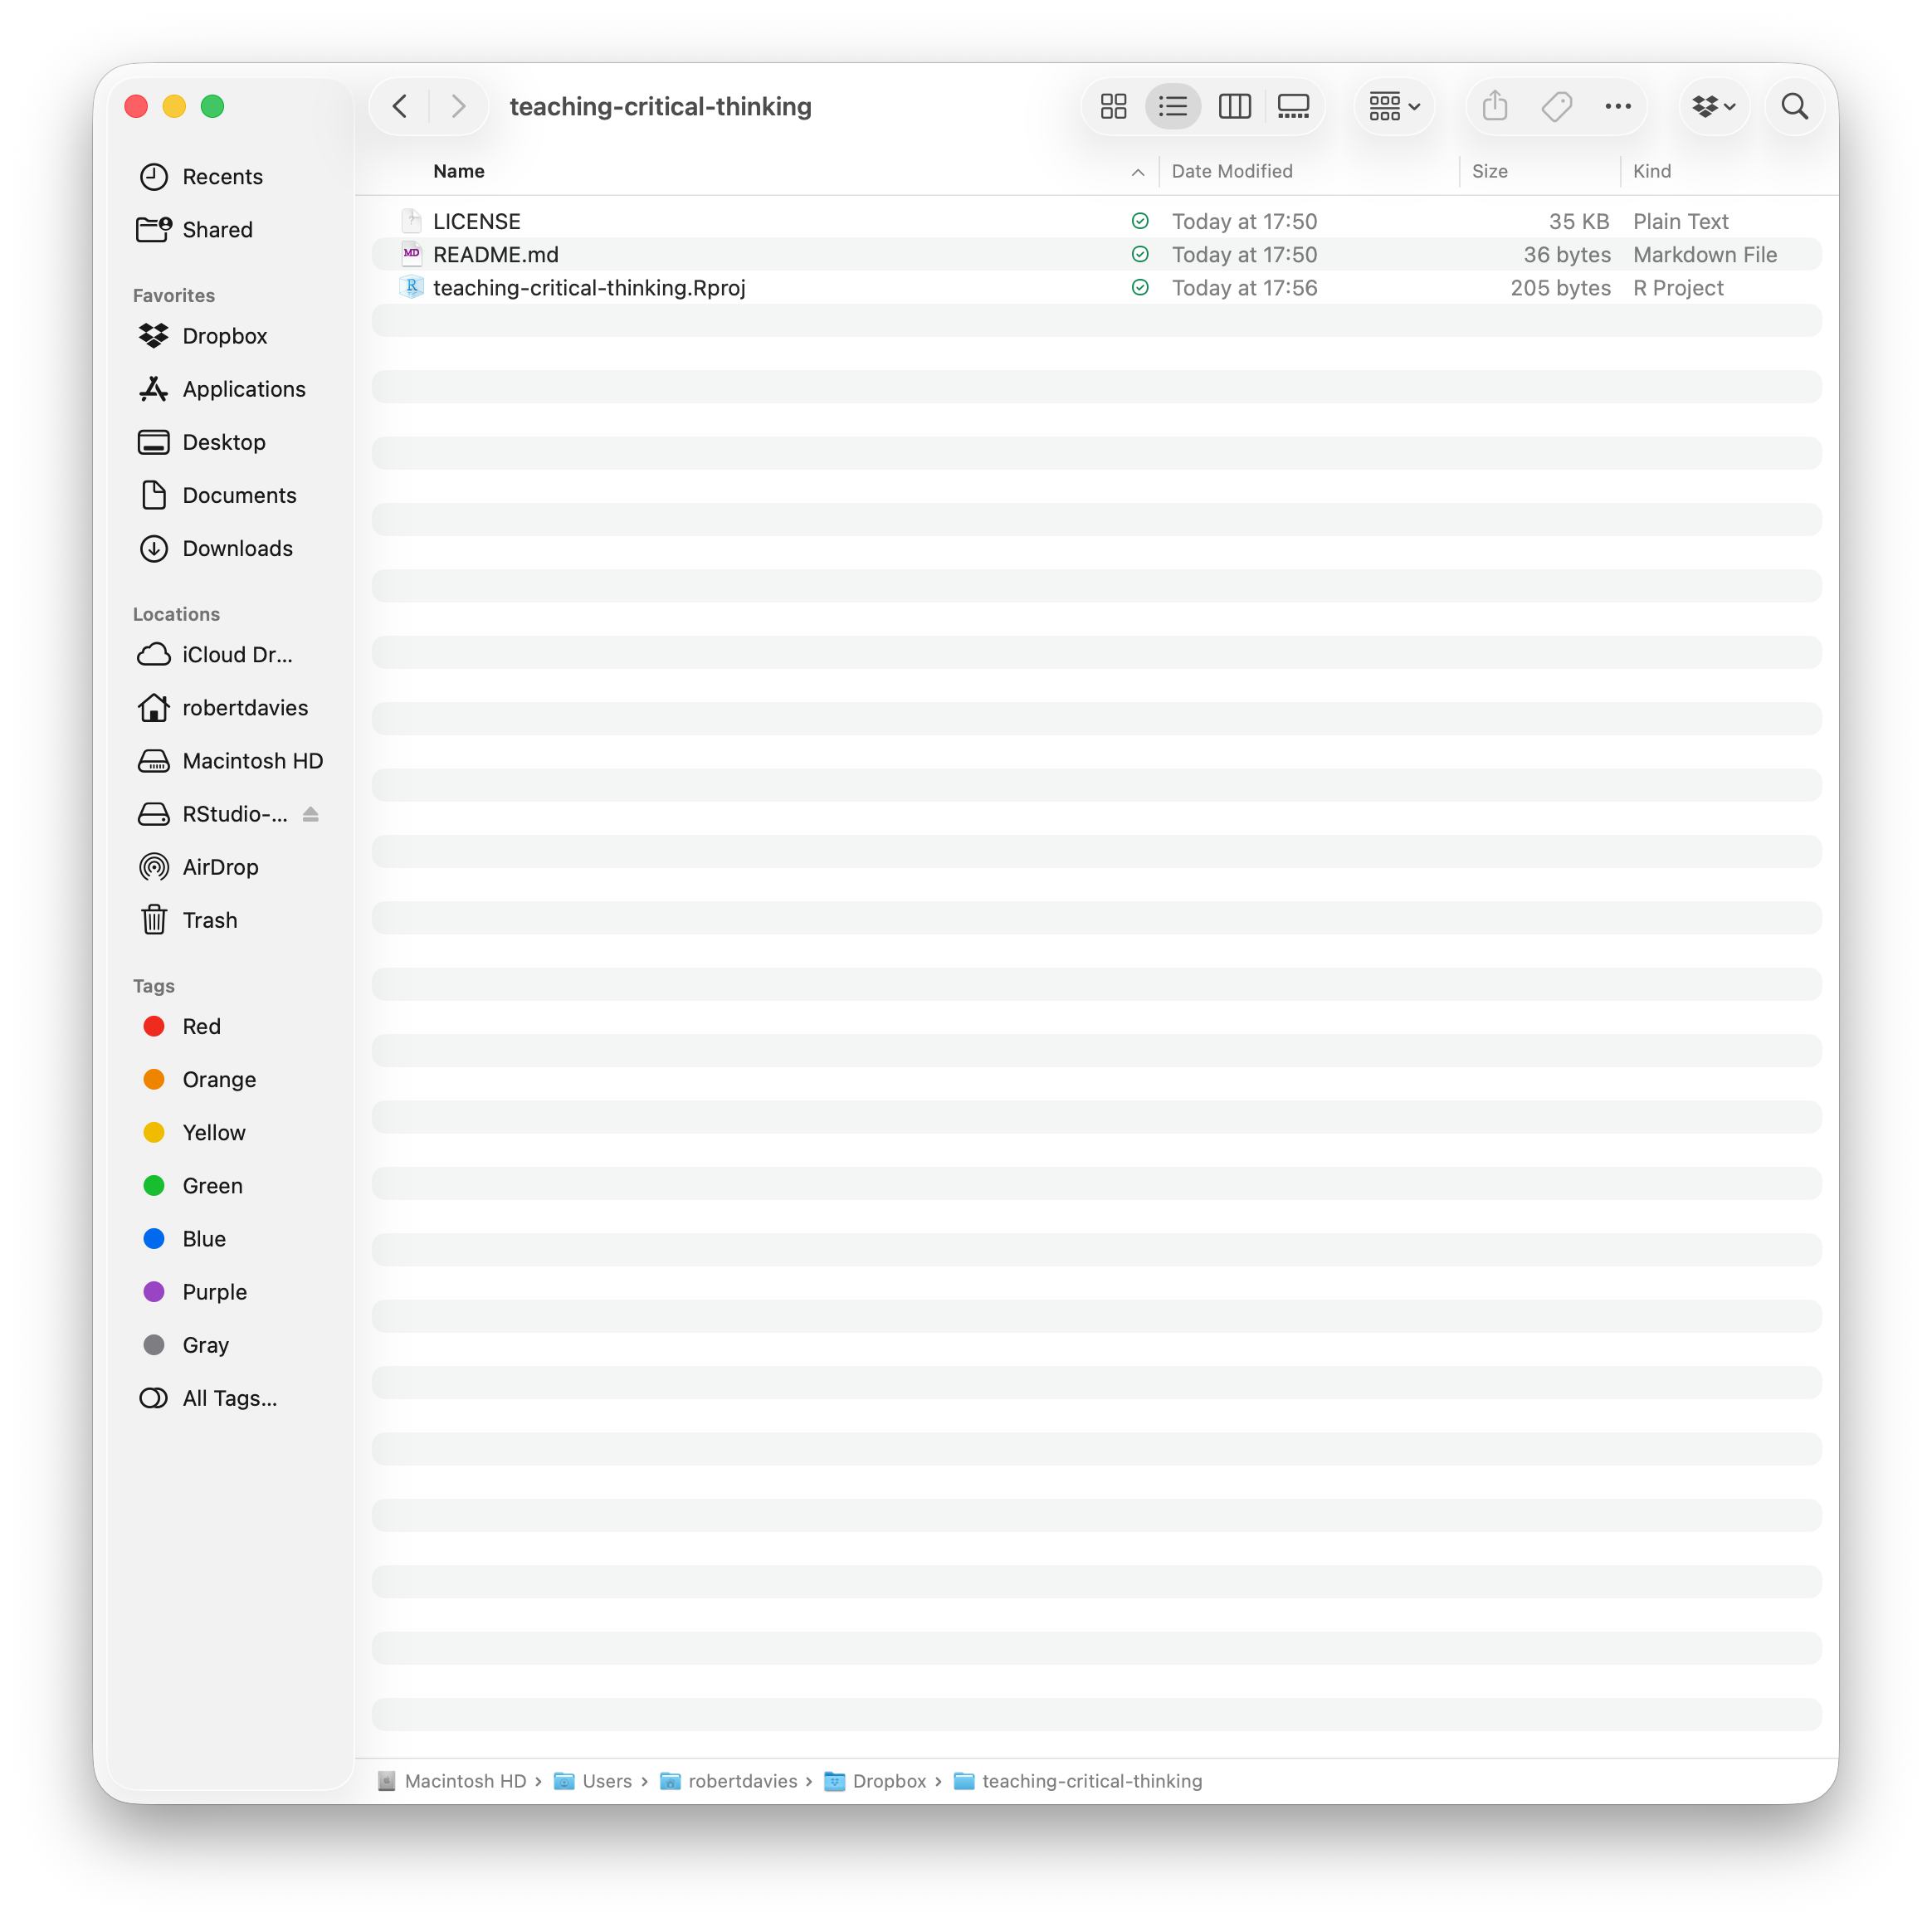
\includegraphics[width=0.6\linewidth,height=\textheight,keepaspectratio]{files/mac-finder-project.png}

}

\caption{\label{fig-mac-finder-project}mac-finder-project}

\end{figure}%

\subsection{Check that our local drive and the remote repository are
connected}\label{check-that-our-local-drive-and-the-remote-repository-are-connected}

Now, in RStudio, you can check that your local drive folder and the
remote repository on GitHub are connected.

\begin{itemize}
\tightlist
\item
  Open the \texttt{README.md}. Edit it. Save the edit.
\item
  Click on the \texttt{Git} tab (top right window). Notice that the
  \texttt{README.md} file is now associated with a blue M under Status.
\end{itemize}

In RStudio \textgreater{} Git

\begin{itemize}
\tightlist
\item
  Click on the button box under \texttt{Staged} to get a tick in the
  box.
\item
  Click on the \texttt{Commit} button above.
\end{itemize}

\begin{figure}

\centering{

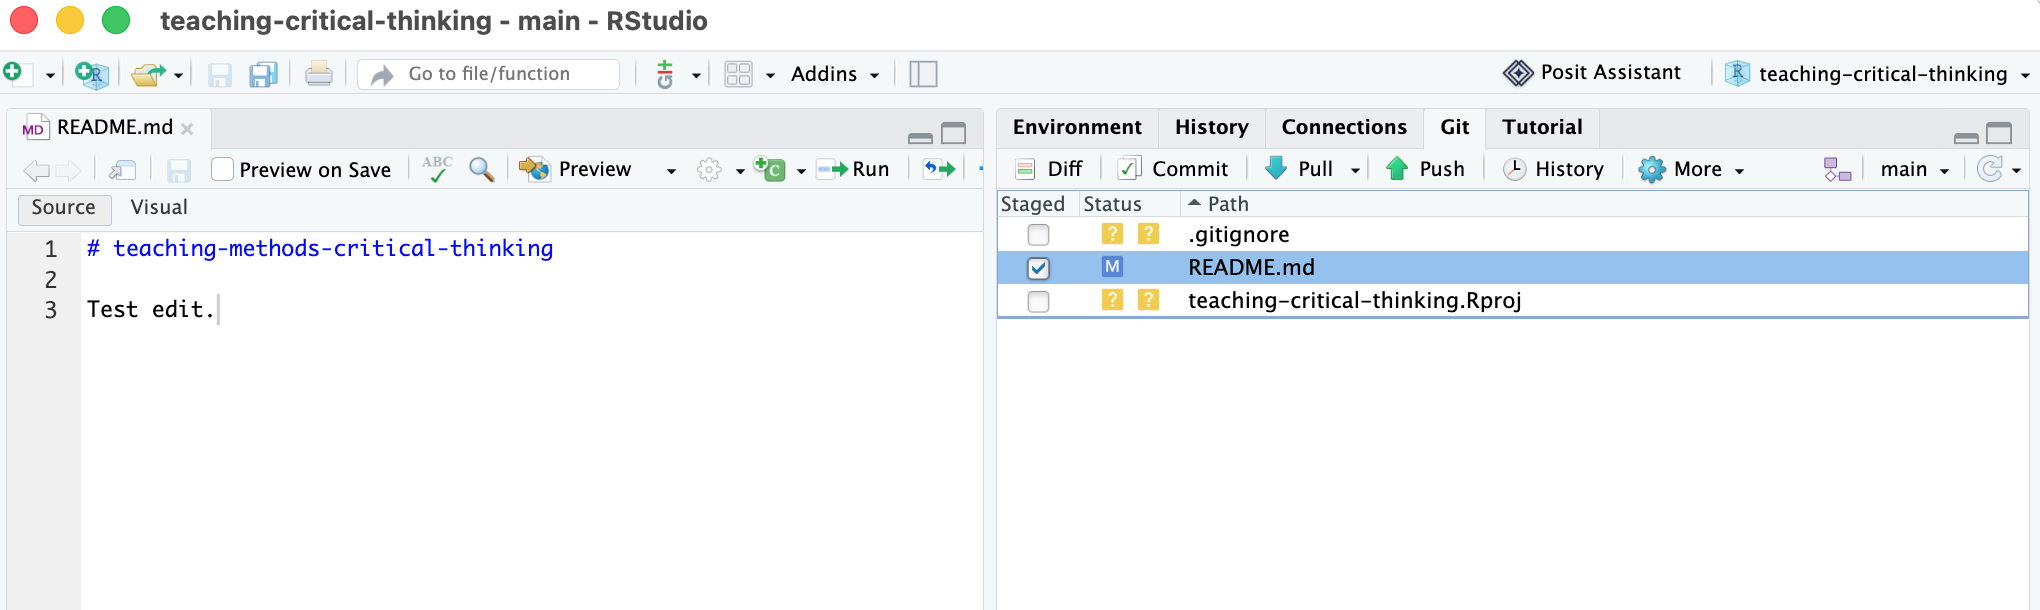
\includegraphics[width=0.6\linewidth,height=\textheight,keepaspectratio]{files/rstudio-git-commit.png}

}

\caption{\label{fig-rstudio-git-commi}rstudio-git-commi}

\end{figure}%

\begin{itemize}
\tightlist
\item
  A window opens.
\item
  Review the changes you have staged. Deletions are shown in red.
  Additions are shown in green.
\item
  Enter a brief but informative message in the commit message box. Click
  on Commit.
\end{itemize}

\begin{figure}

\centering{

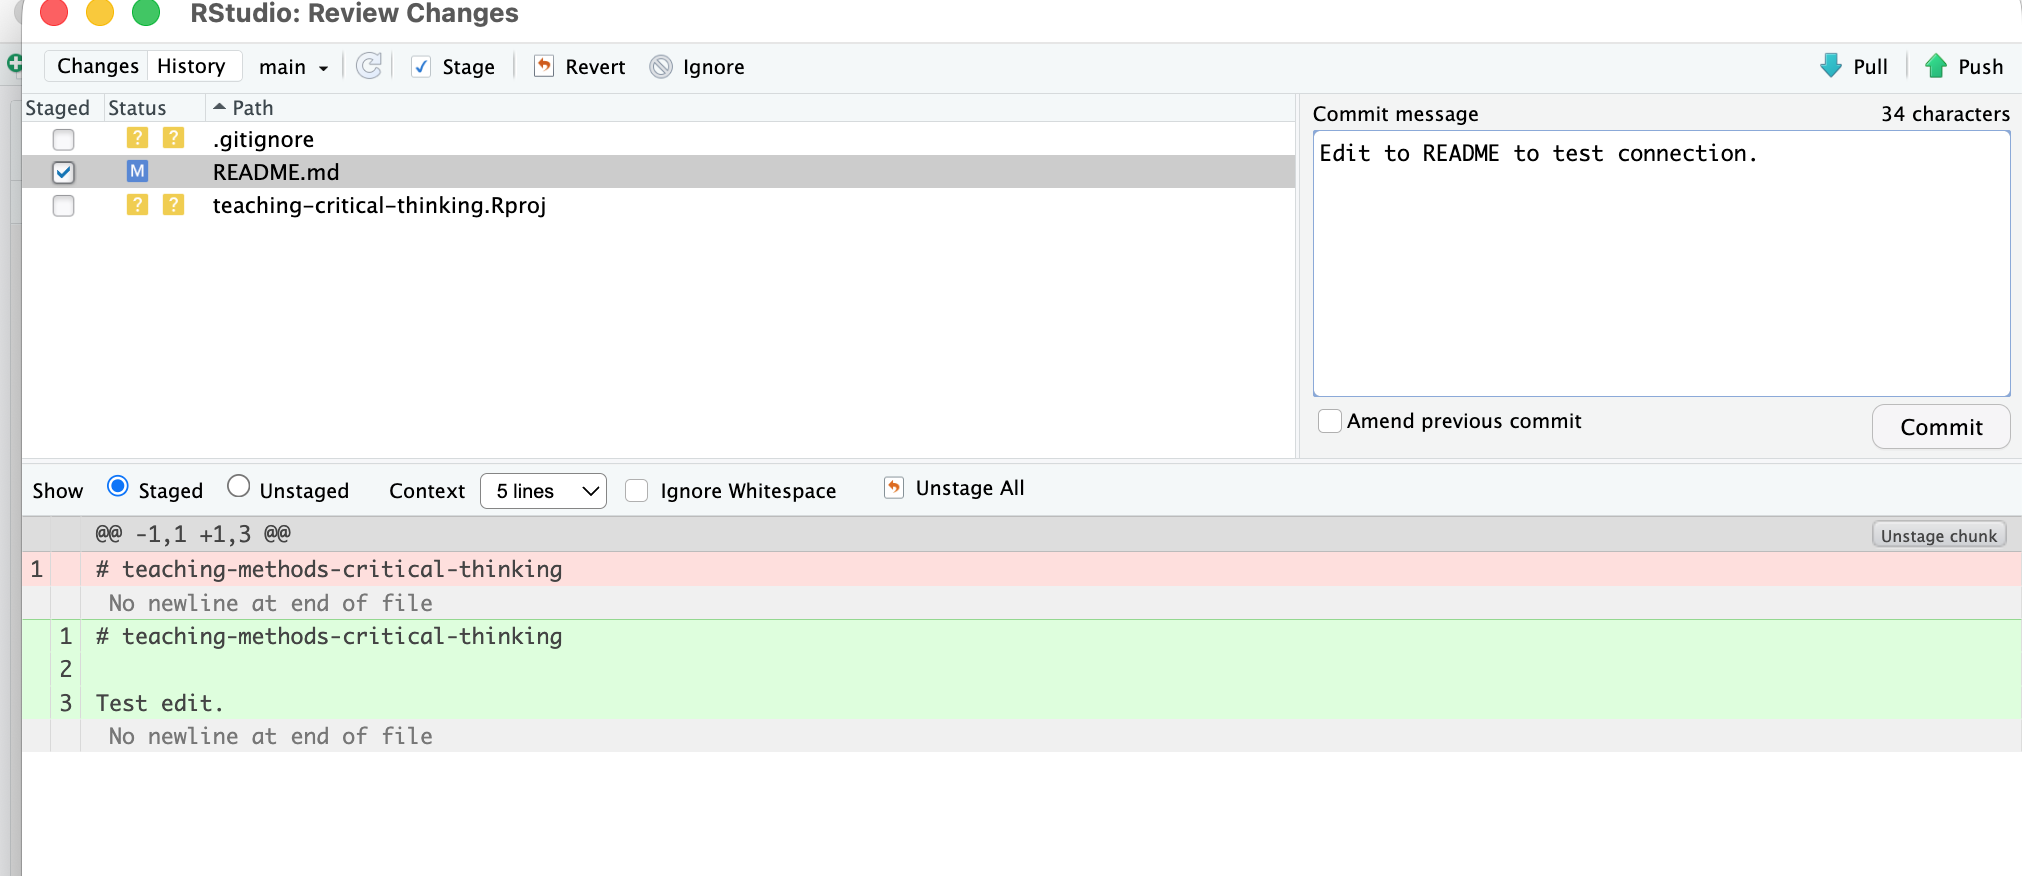
\includegraphics[width=0.6\linewidth,height=\textheight,keepaspectratio]{files/rstudio-git-commit-message.png}

}

\caption{\label{fig-rstudio-git-commit-message}rstudio-git-commit-message}

\end{figure}%

\begin{itemize}
\item
  Best practice advice is to commit often, push less frequently.
\item
  RStudio \textgreater{} Git We click on \texttt{Push} to test the
  connection.
\end{itemize}

Assuming the connection is good, clicking on the \texttt{Push} will show
you a window showing a summary of what has been changed in (pushed up
to) the repo.

\begin{figure}

\centering{

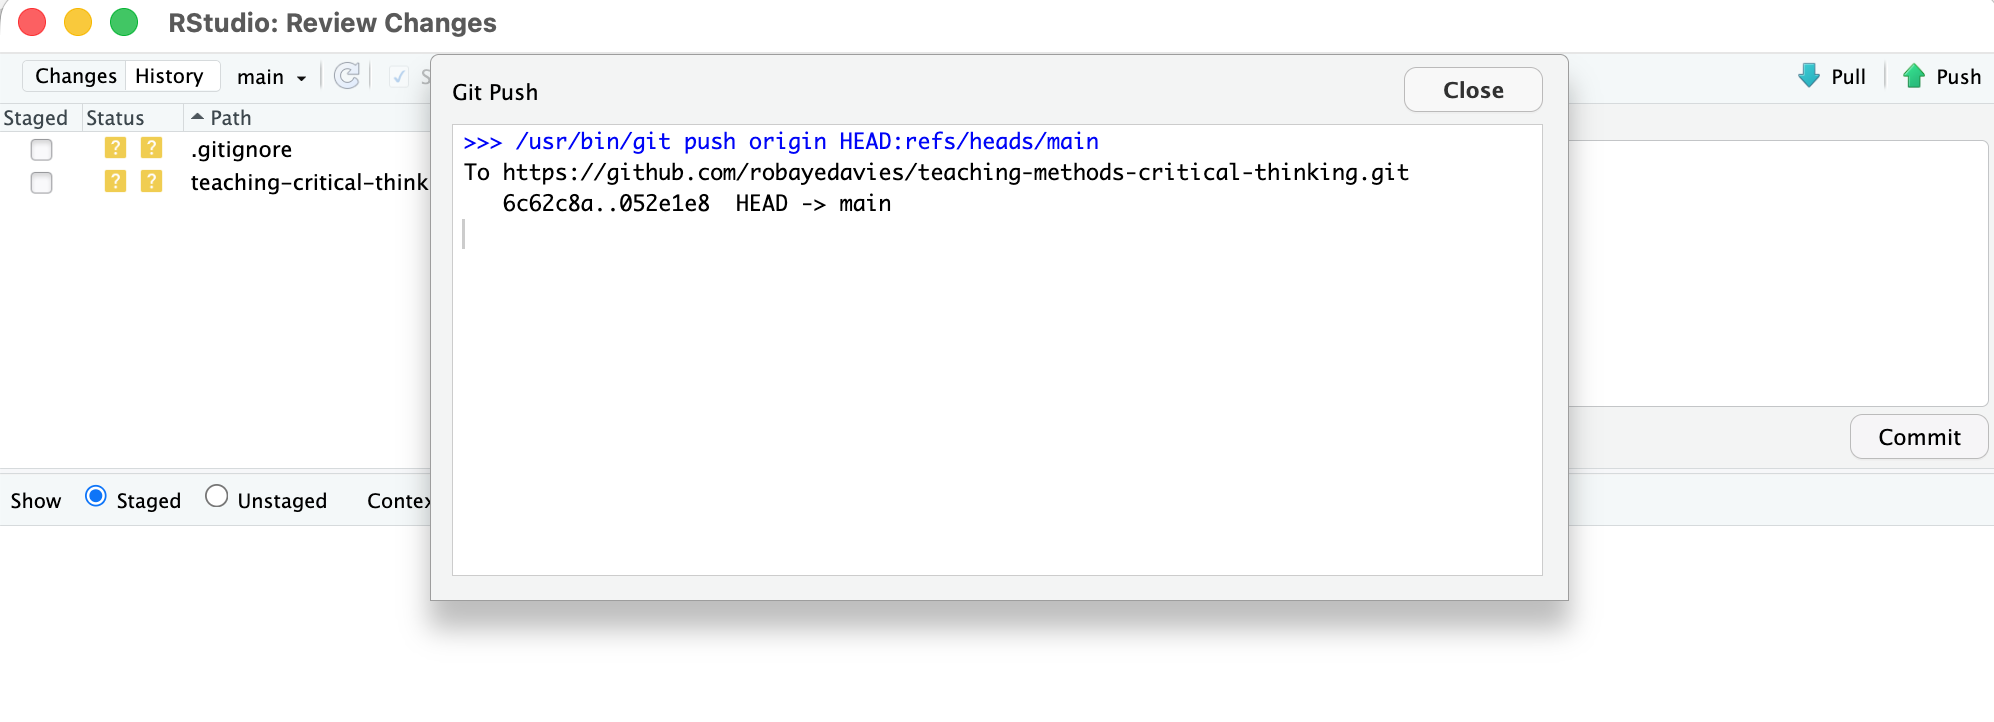
\includegraphics[width=0.6\linewidth,height=\textheight,keepaspectratio]{files/rstudio-git-commit-message-push.png}

}

\caption{\label{fig-rstudio-git-commit-message-push}rstudio-git-commit-message-push}

\end{figure}%

Now, in GitHub, you can check that your local drive folder and the
remote repository on GitHub are connected.

\begin{itemize}
\tightlist
\item
  At the repo webpage, you can see the commit message, a with a
  timestamp.
\item
  This is why it is wise to write informative messages: you want to know
  what you did when.
\item
  You can click on a file name to see the edits.
\end{itemize}

\begin{figure}

\centering{

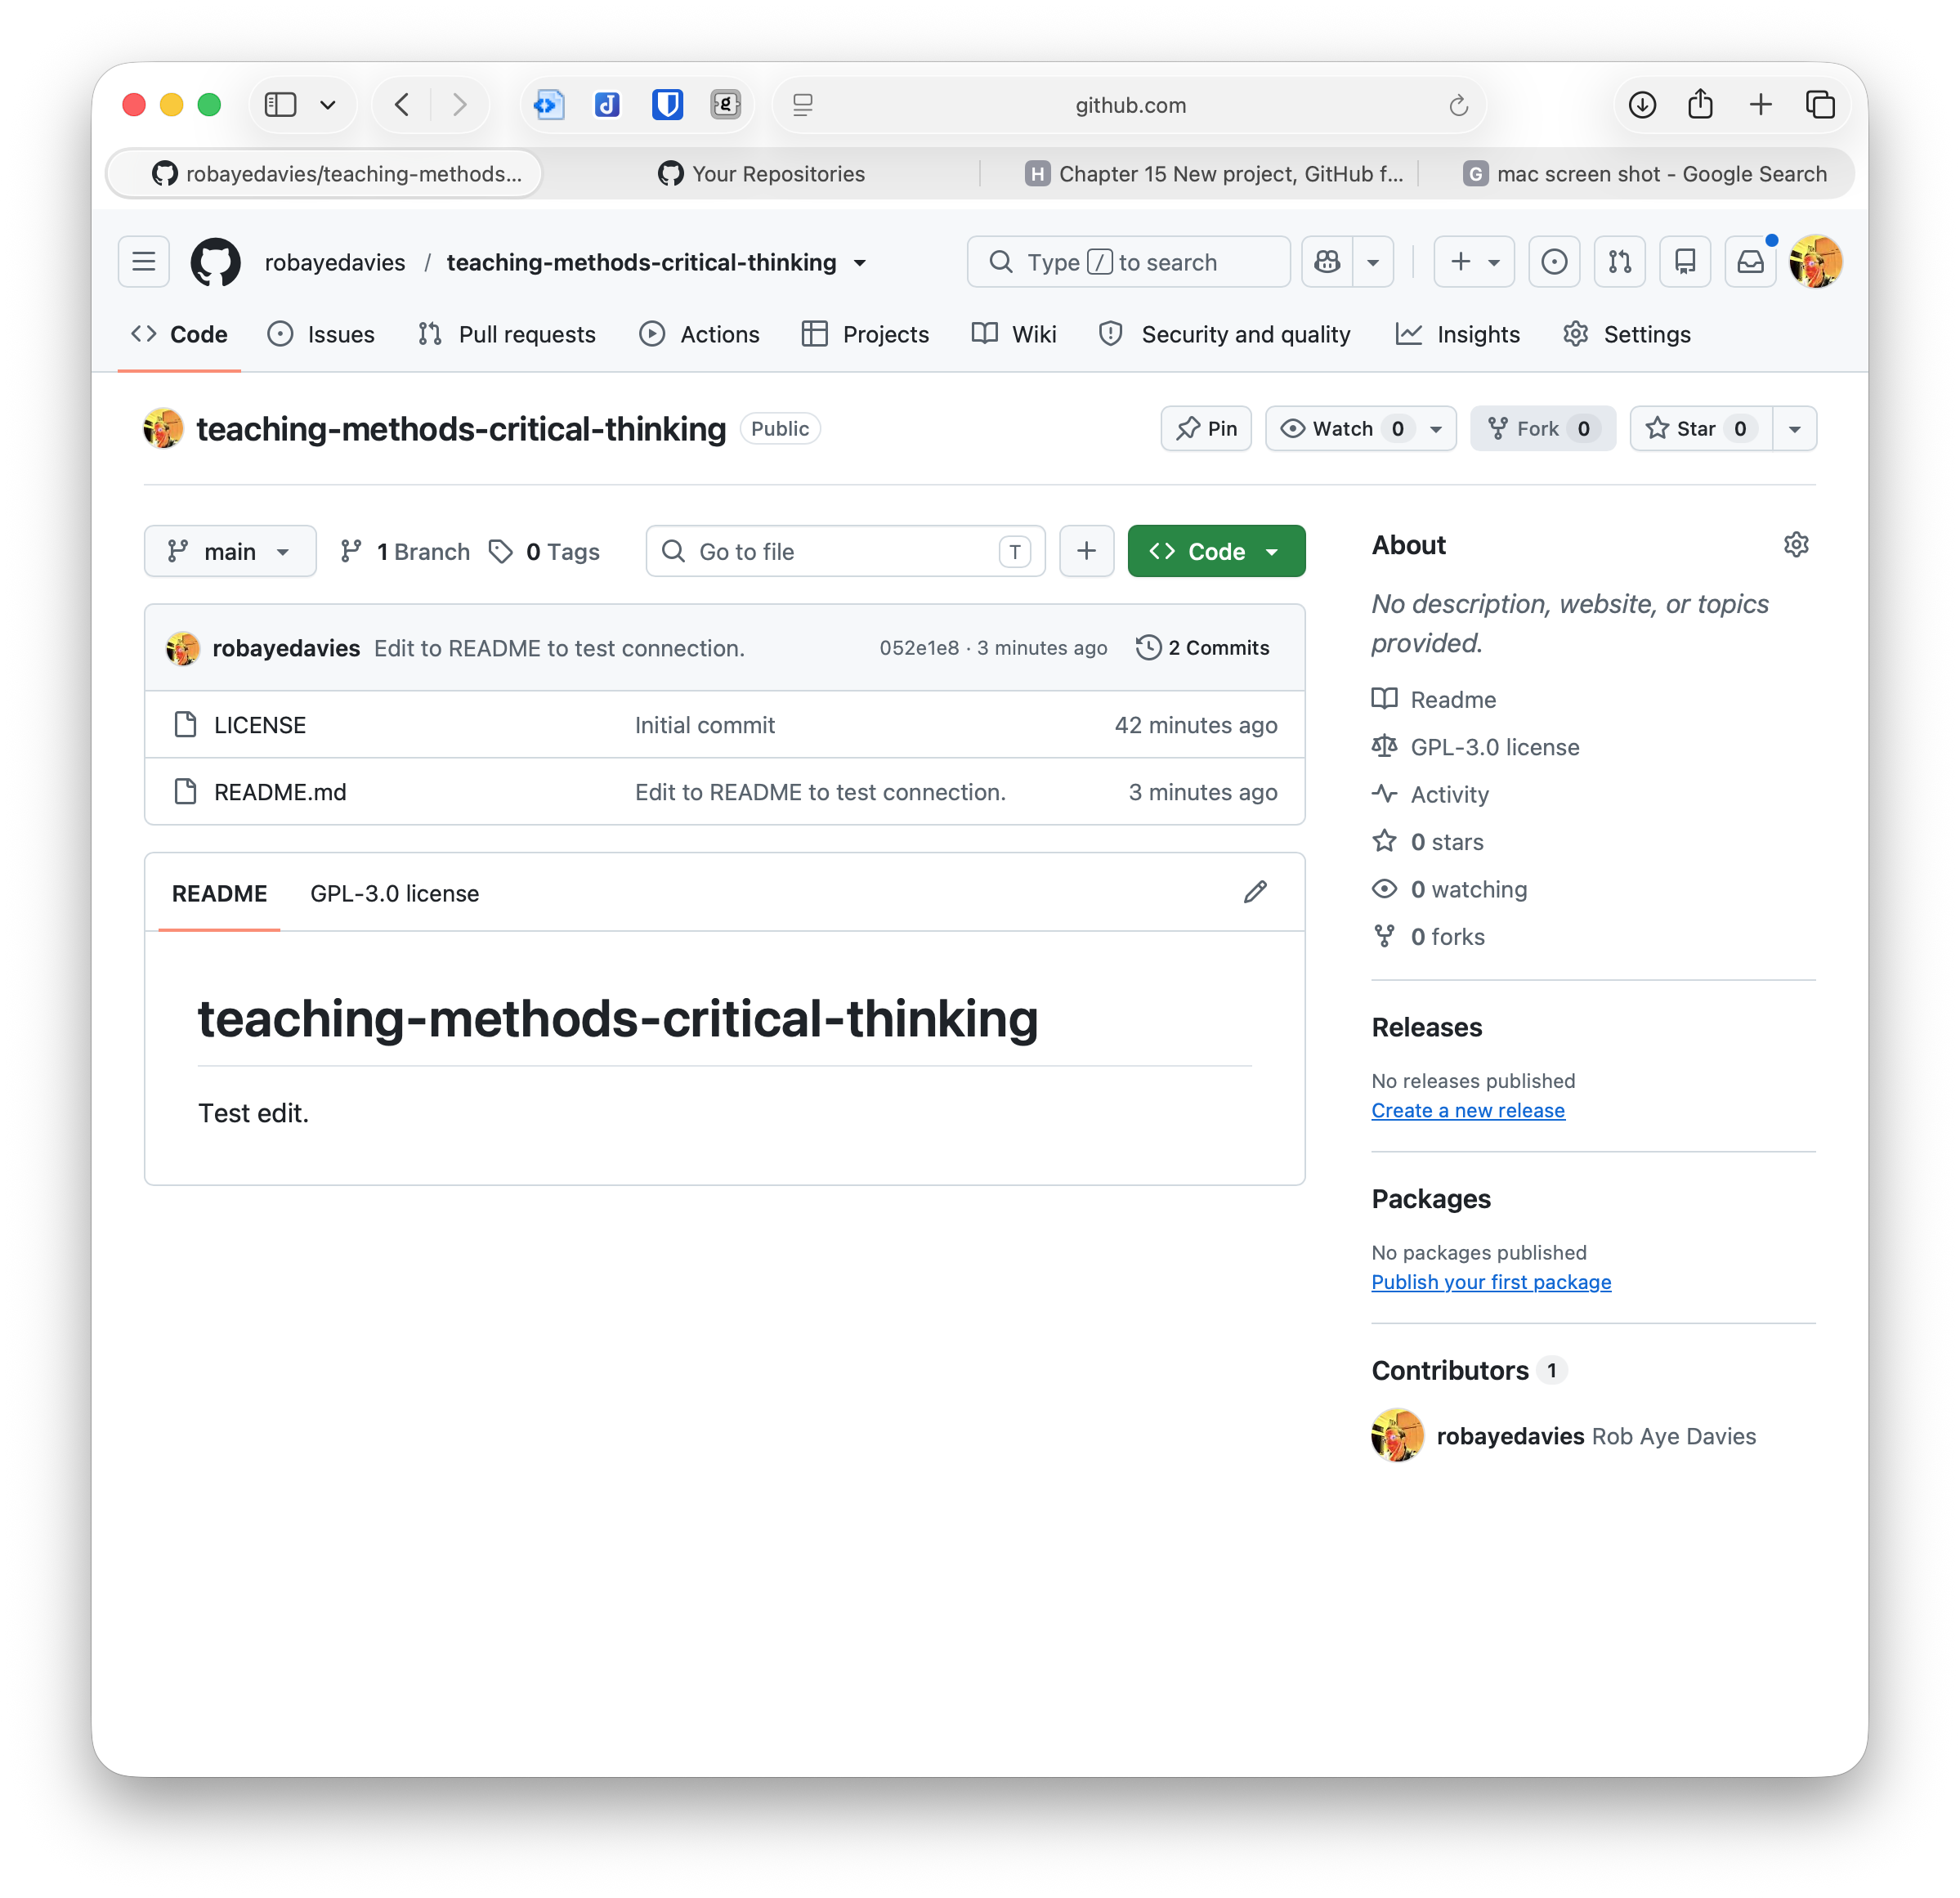
\includegraphics[width=0.6\linewidth,height=\textheight,keepaspectratio]{files/github-commits-edits.png}

}

\caption{\label{fig-github-commits-edits}github-commits-edits}

\end{figure}%

That was pushing. How about pulling?

\begin{itemize}
\tightlist
\item
  Click on the \texttt{Pull} button.
\end{itemize}

\begin{figure}

\centering{

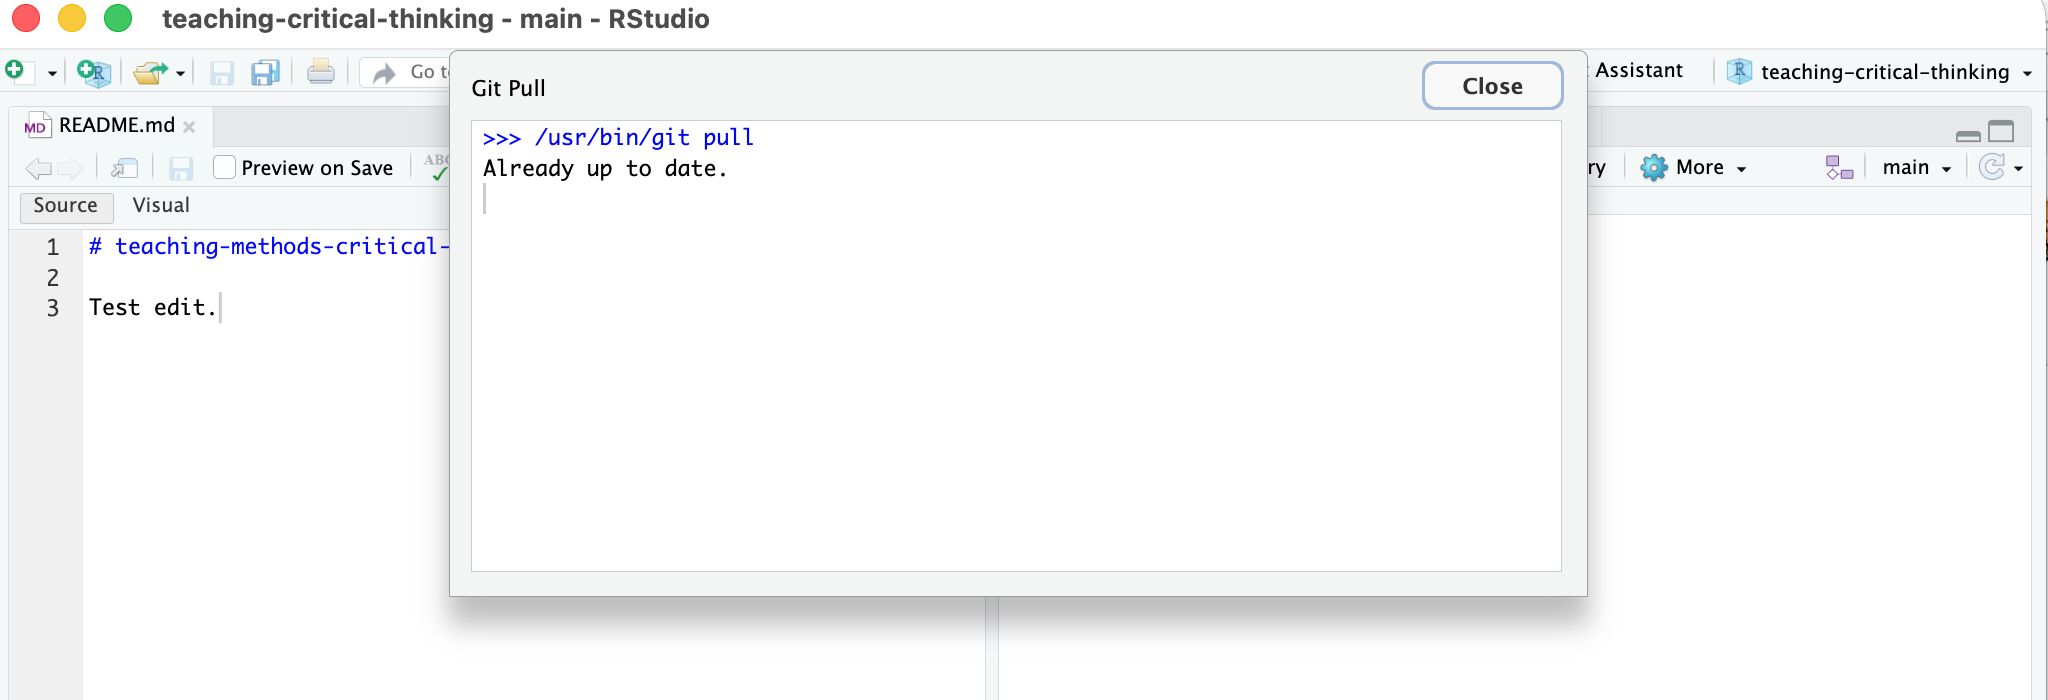
\includegraphics[width=0.6\linewidth,height=\textheight,keepaspectratio]{files/rstudio-git-pull.png}

}

\caption{\label{fig-rstudio-git-pull}rstudio-git-pulln}

\end{figure}%

\begin{itemize}
\tightlist
\item
  It works i.e.~you can get changes to the repository downloaded to your
  local drive but there are no changes and everything is up to date.
\end{itemize}

\subsection{Create a new book}\label{create-a-new-book}

Let's say I don't already have a book but I want to create a book, and I
want to make a Quarto book. We can create a set of files to act as a
skeleton for the book we are going to write.

In RStudio, in the terminal, we write the command:

\begin{Shaded}
\begin{Highlighting}[]
\ExtensionTok{quarto}\NormalTok{ create project book .}
\end{Highlighting}
\end{Shaded}

The trailing dot tells Quarto to use the current directory rather than
making a new subfolder.

\begin{itemize}
\tightlist
\item
  You will be asked to enter a title.
\end{itemize}

In the terminal, you will see results that look like this. The directory
information will be different.

\begin{figure}

\centering{

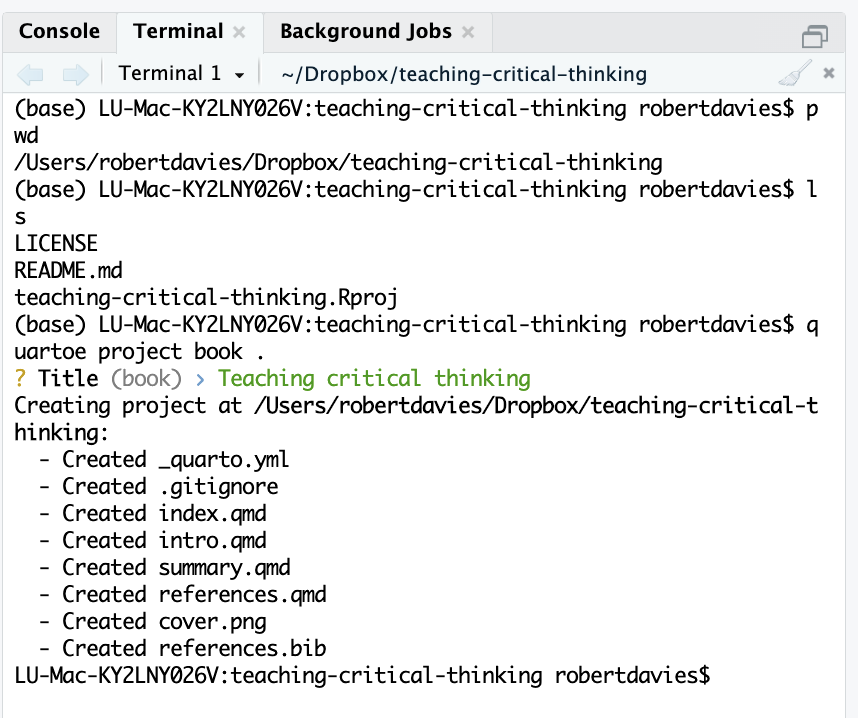
\includegraphics[width=0.6\linewidth,height=\textheight,keepaspectratio]{files/rstudio-terminal-quarto-create-book.png}

}

\caption{\label{fig-rstudio-terminal-quarto-create-book}rstudio-terminal-quarto-create-book}

\end{figure}%

This bash code (a sequence of code entered at the terminal) creates
\_quarto.yml, index.qmd, intro.qmd, summary.qmd, references.qmd, and
references.bib.

\begin{itemize}
\tightlist
\item
  You can see these files have appeared in the folder you are working
  with.
\end{itemize}

\begin{figure}

\centering{

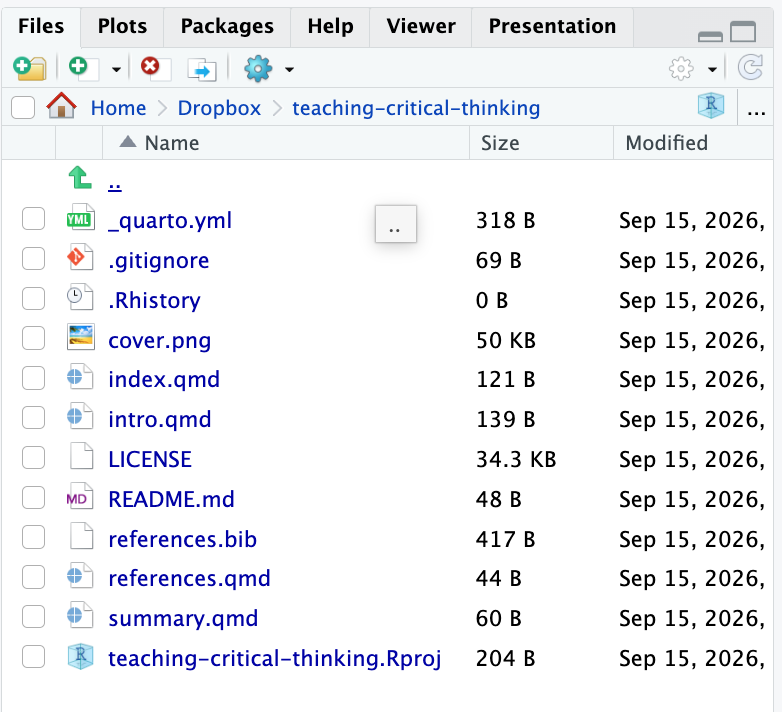
\includegraphics[width=0.6\linewidth,height=\textheight,keepaspectratio]{files/rstudio-files-project-book-files.png}

}

\caption{\label{fig-rstudio-files-project-book-files}rstudio-files-project-book-files}

\end{figure}%

\subsection{Working with the book
yaml}\label{working-with-the-book-yaml}

In RStudio, in the script window, in the open \texttt{\_quarto.yml}
file, we can see some pre-populated information and the title we
entered.

\begin{figure}

\centering{

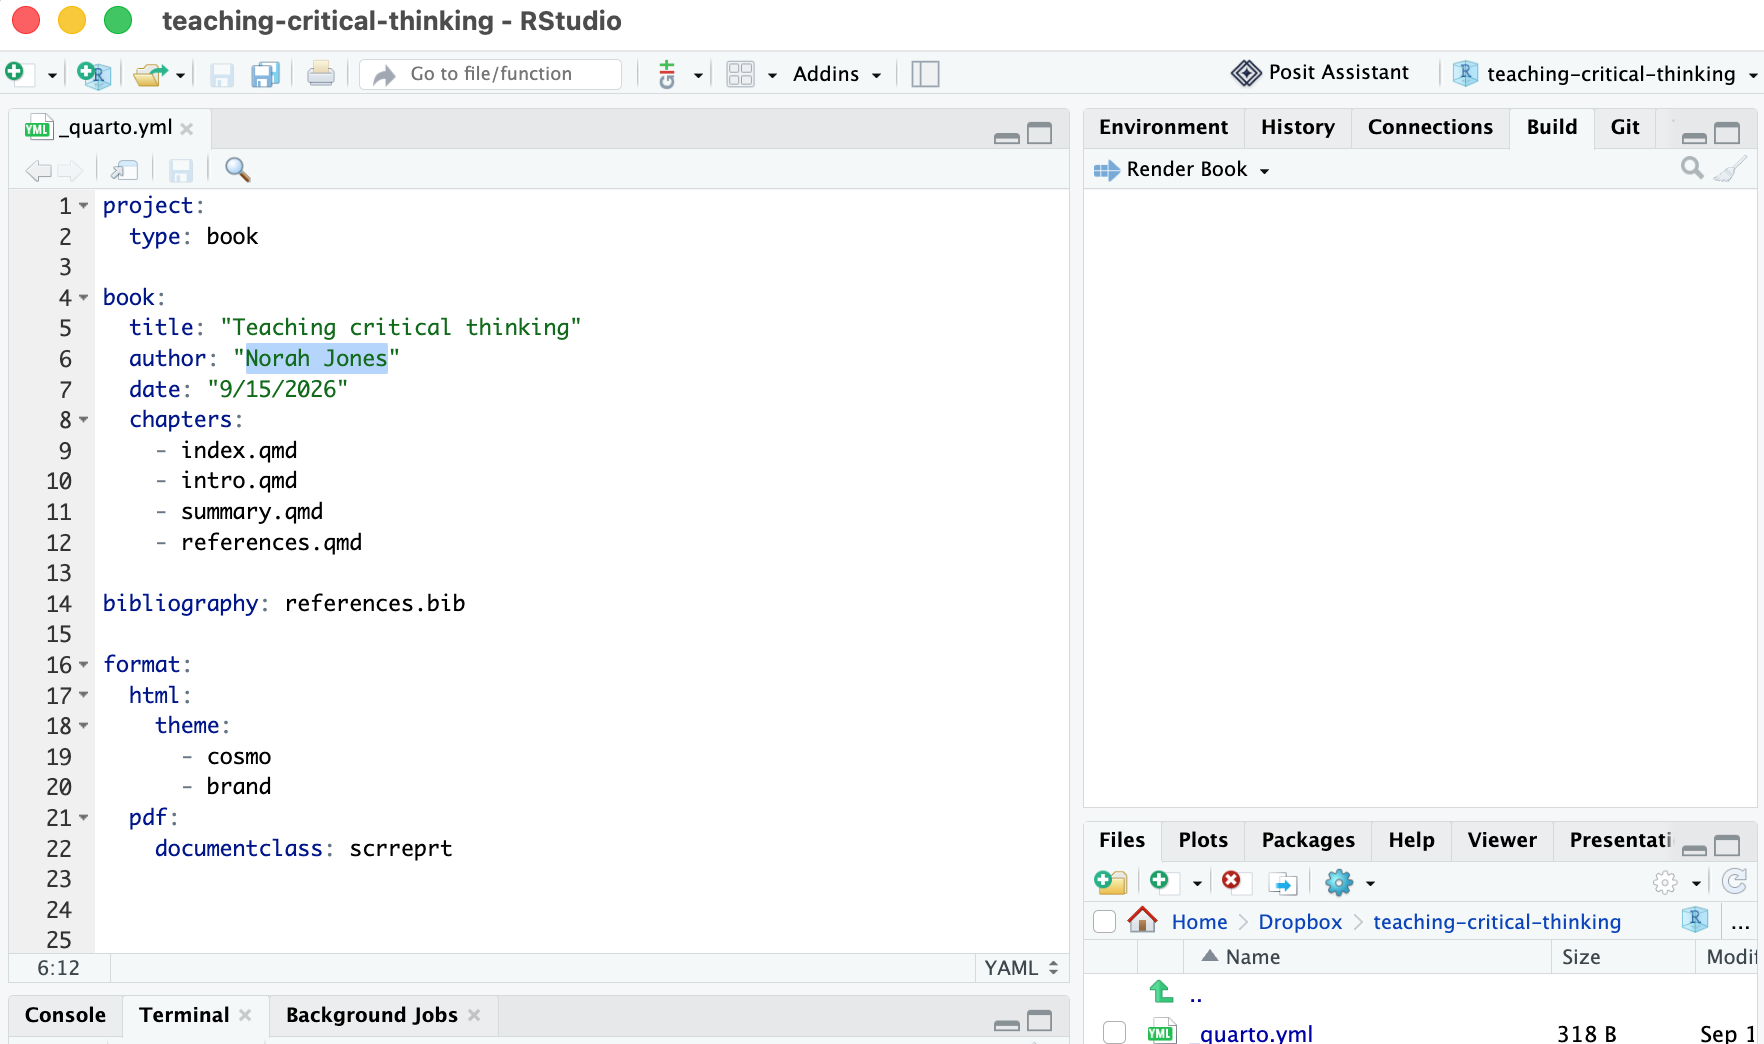
\includegraphics[width=0.6\linewidth,height=\textheight,keepaspectratio]{files/rstudio-script-yaml-defaults.png}

}

\caption{\label{fig-rstudio-script-yaml-defaults}rstudio-script-yaml-defaults}

\end{figure}%

\begin{itemize}
\tightlist
\item
  Edit the yaml to substitute the prepopulated author name with your
  name.
\item
  Save.
\end{itemize}

\subsection{Preview what we have got so
far.}\label{preview-what-we-have-got-so-far.}

Click on \texttt{Render} in RStudio, or run \texttt{quarto\ preview} in
the Terminal.

Your default browser will open a live preview that updates as you edit
and save .qmd files.

Let's say I run \texttt{quarto\ preview} in the terminal. This is what I
see in the terminal.

\begin{figure}

\centering{

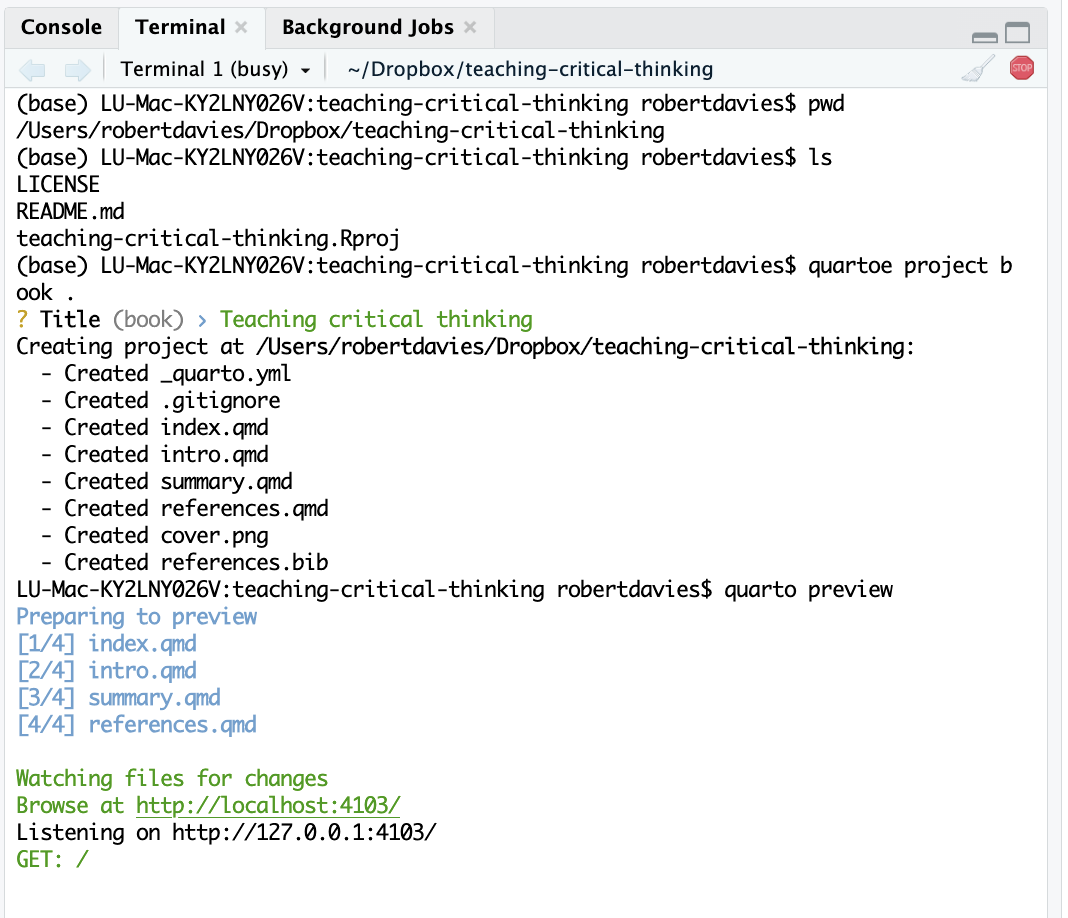
\includegraphics[width=0.6\linewidth,height=\textheight,keepaspectratio]{files/rstudio-terminal-quarto-preview.png}

}

\caption{\label{fig-rstudio-terminal-quarto-preview}rstudio-terminal-quarto-preview}

\end{figure}%

A new webpage tab should open. Here is what Safari shows me:

\begin{figure}

\centering{

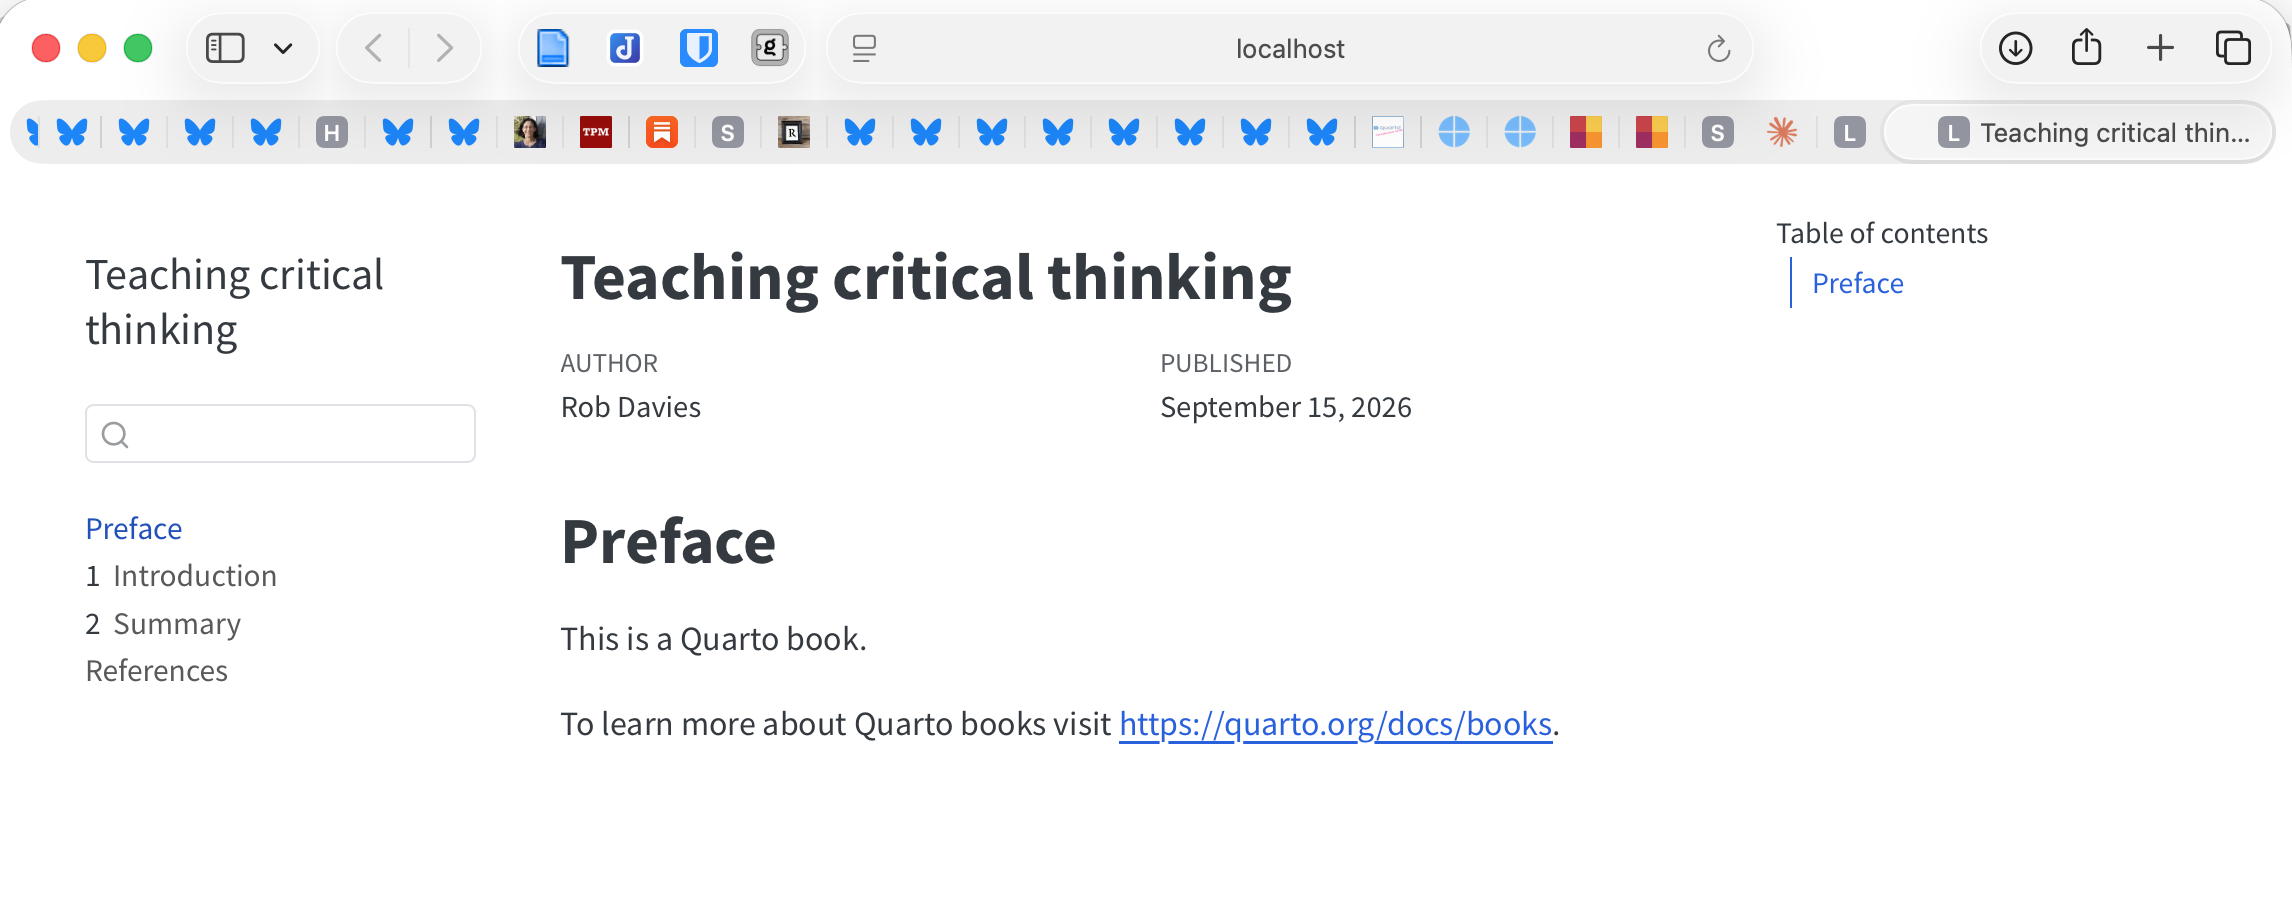
\includegraphics[width=0.6\linewidth,height=\textheight,keepaspectratio]{files/safari-browser-quarto-preview.png}

}

\caption{\label{fig-safari-browser-quarto-preview}safari-browser-quarto-preview}

\end{figure}%

Notice that in RStudio \textgreater{} Terminal, you can see a red button
and the message

\begin{verbatim}
Watching files for changes
Browse at http://localhost:5105/
Listening on http://127.0.0.1:5105/
GET: /
\end{verbatim}

\begin{itemize}
\tightlist
\item
  Click on the red button and the Preview stops.
\end{itemize}

This preview is local to you. In the next step, we publish what we have
got so far so anyone can view it, if they have the URL.

There are two ways to do this:

\begin{enumerate}
\def\labelenumi{\arabic{enumi}.}
\tightlist
\item
  The simplest: run \texttt{quarto\ publish\ gh-pages} from the
  Terminal. This renders the book, pushes it to an auto-created
  \texttt{gh-pages} branch, and \texttt{GitHub\ Pages} picks it up
  automatically.
\item
  Alternative: set `output-dir: docs' in \_quarto.yml, render, commit
  the docs/ folder, add a .nojekyll file, and point GitHub Pages at the
  docs/ folder in Settings \textgreater{} Pages.
\end{enumerate}

I am going to use the second route.

\subsection{Publish your new book to live
webpages}\label{publish-your-new-book-to-live-webpages}

In Rstudio, in the script window, in \texttt{\_quarto.yml}, set the
output directory.

\begin{itemize}
\tightlist
\item
  Edit the yaml, adding on a new line: \texttt{output-dir:\ docs}.
\end{itemize}

\begin{figure}

\centering{

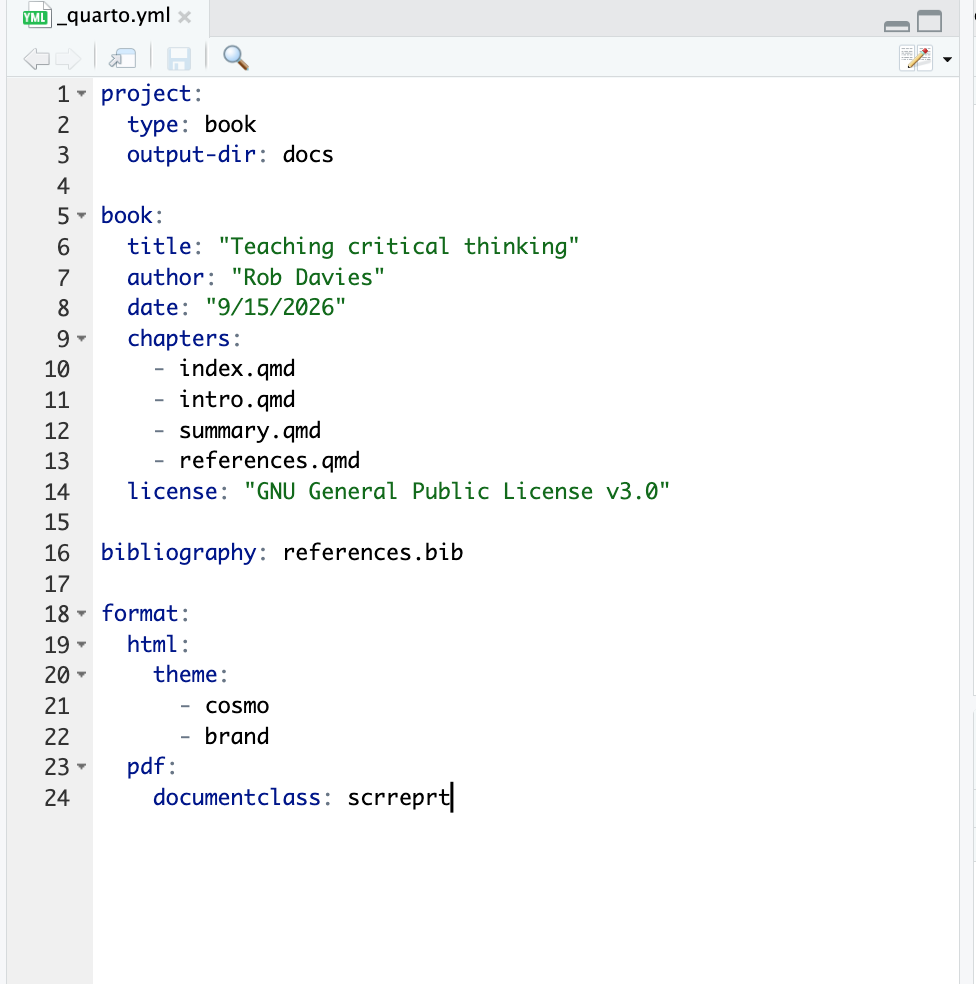
\includegraphics[width=0.6\linewidth,height=\textheight,keepaspectratio]{files/rstudio-script-yaml-book-docs.png}

}

\caption{\label{fig-rstudio-script-yaml-book-docs}rstudio-script-yaml-book-docs}

\end{figure}%

In Rstudio, in the terminal, enter \texttt{touch\ .nojekyll}.

Add a .nojekyll file to your repo root (touch .nojekyll in Terminal, or
copy NUL .nojekyll on Windows). This stops GitHub from running its own
Jekyll processor over your site, which can break Quarto's output.

In Rstudio, in the terminal, \texttt{quarto\ render}.

\begin{itemize}
\tightlist
\item
  The terminal will display its progress through the rendering process.
\item
  A review of the contents of the folder will show the new /docs/
  folder.
\end{itemize}

In Rstudio, in git, commit all the new files. Then push.

\begin{figure}

\centering{

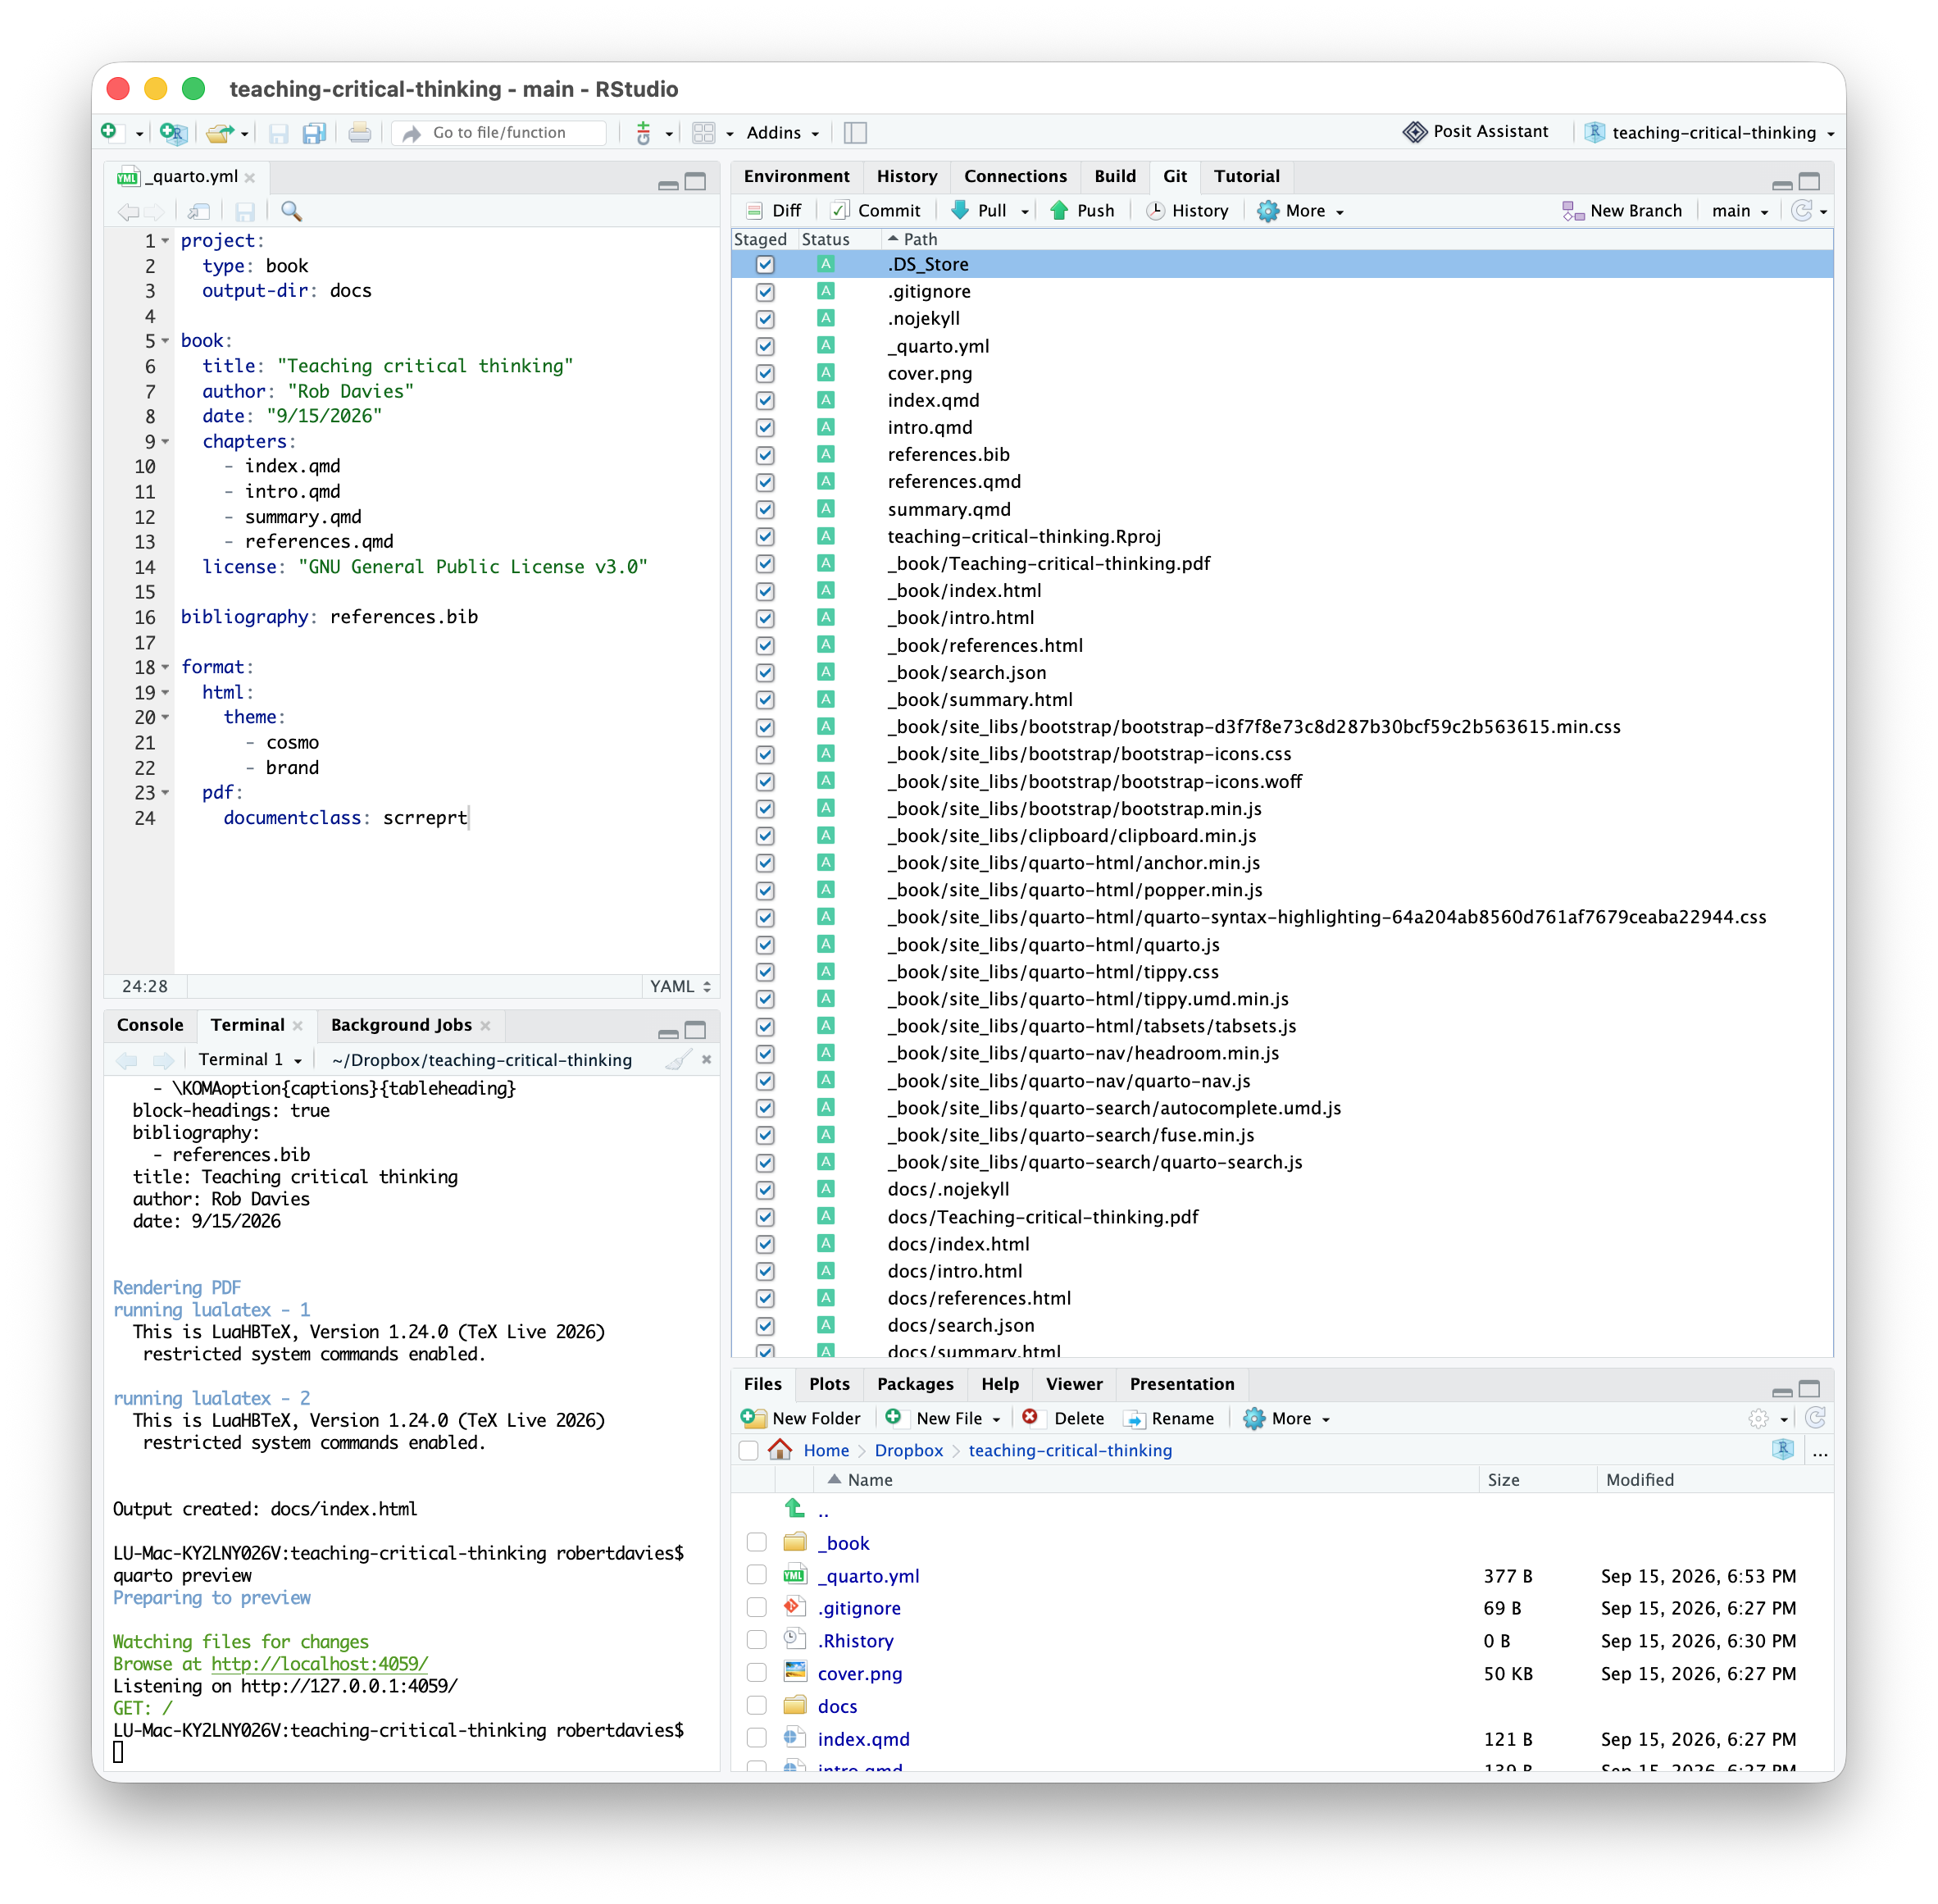
\includegraphics[width=0.6\linewidth,height=\textheight,keepaspectratio]{files/rstudio-git-commit-new-all.png}

}

\caption{\label{fig-rstudio-git-commit-new-all}rstudio-git-commit-new-all}

\end{figure}%

Commit all new book files.

\subsubsection{Fix the license}\label{fix-the-license}

We might not have already done this but we need to choose a license for
our materials.

In GitHub, change the license to CC.0

Before doing anything else, I pull this remote change to the local
version.

\begin{figure}

\centering{

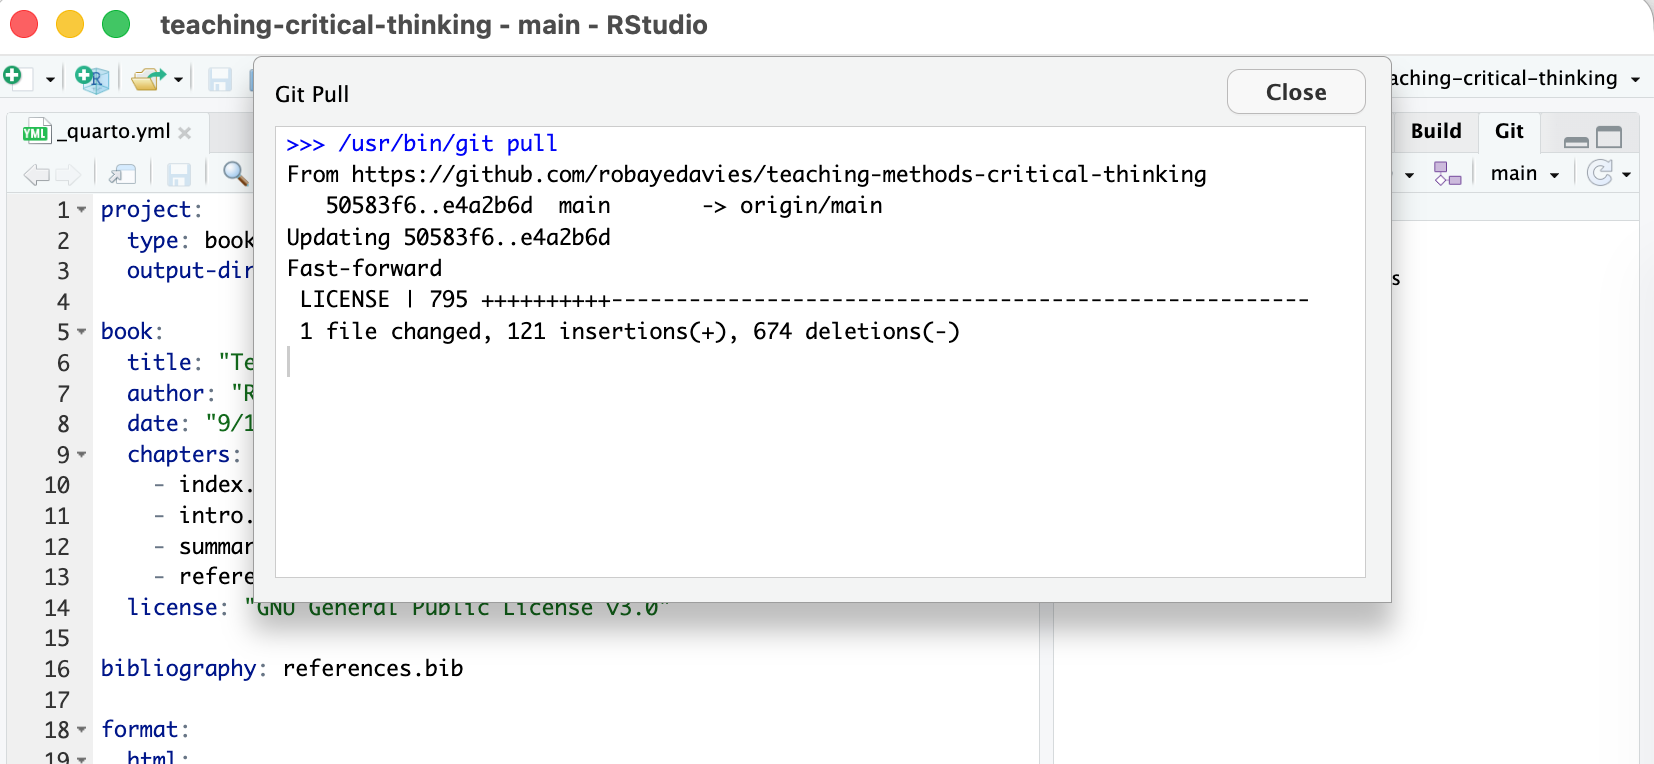
\includegraphics[width=0.6\linewidth,height=\textheight,keepaspectratio]{files/rstudio-git-pull-license-edit.png}

}

\caption{\label{fig-rstudio-git-pull-license-edit}rstudio-git-pull-license-edit}

\end{figure}%

\subsubsection{Publish the book}\label{publish-the-book}

Point GitHub Pages at /docs

On GitHub.com, go to your repo's Settings \textgreater{} Pages. Under
\texttt{Build\ and\ deployment}, set Source to
\texttt{Deploy\ from\ a\ branch}, Branch to \texttt{main}, and folder to
\texttt{/docs}. Save.

\begin{figure}

\centering{

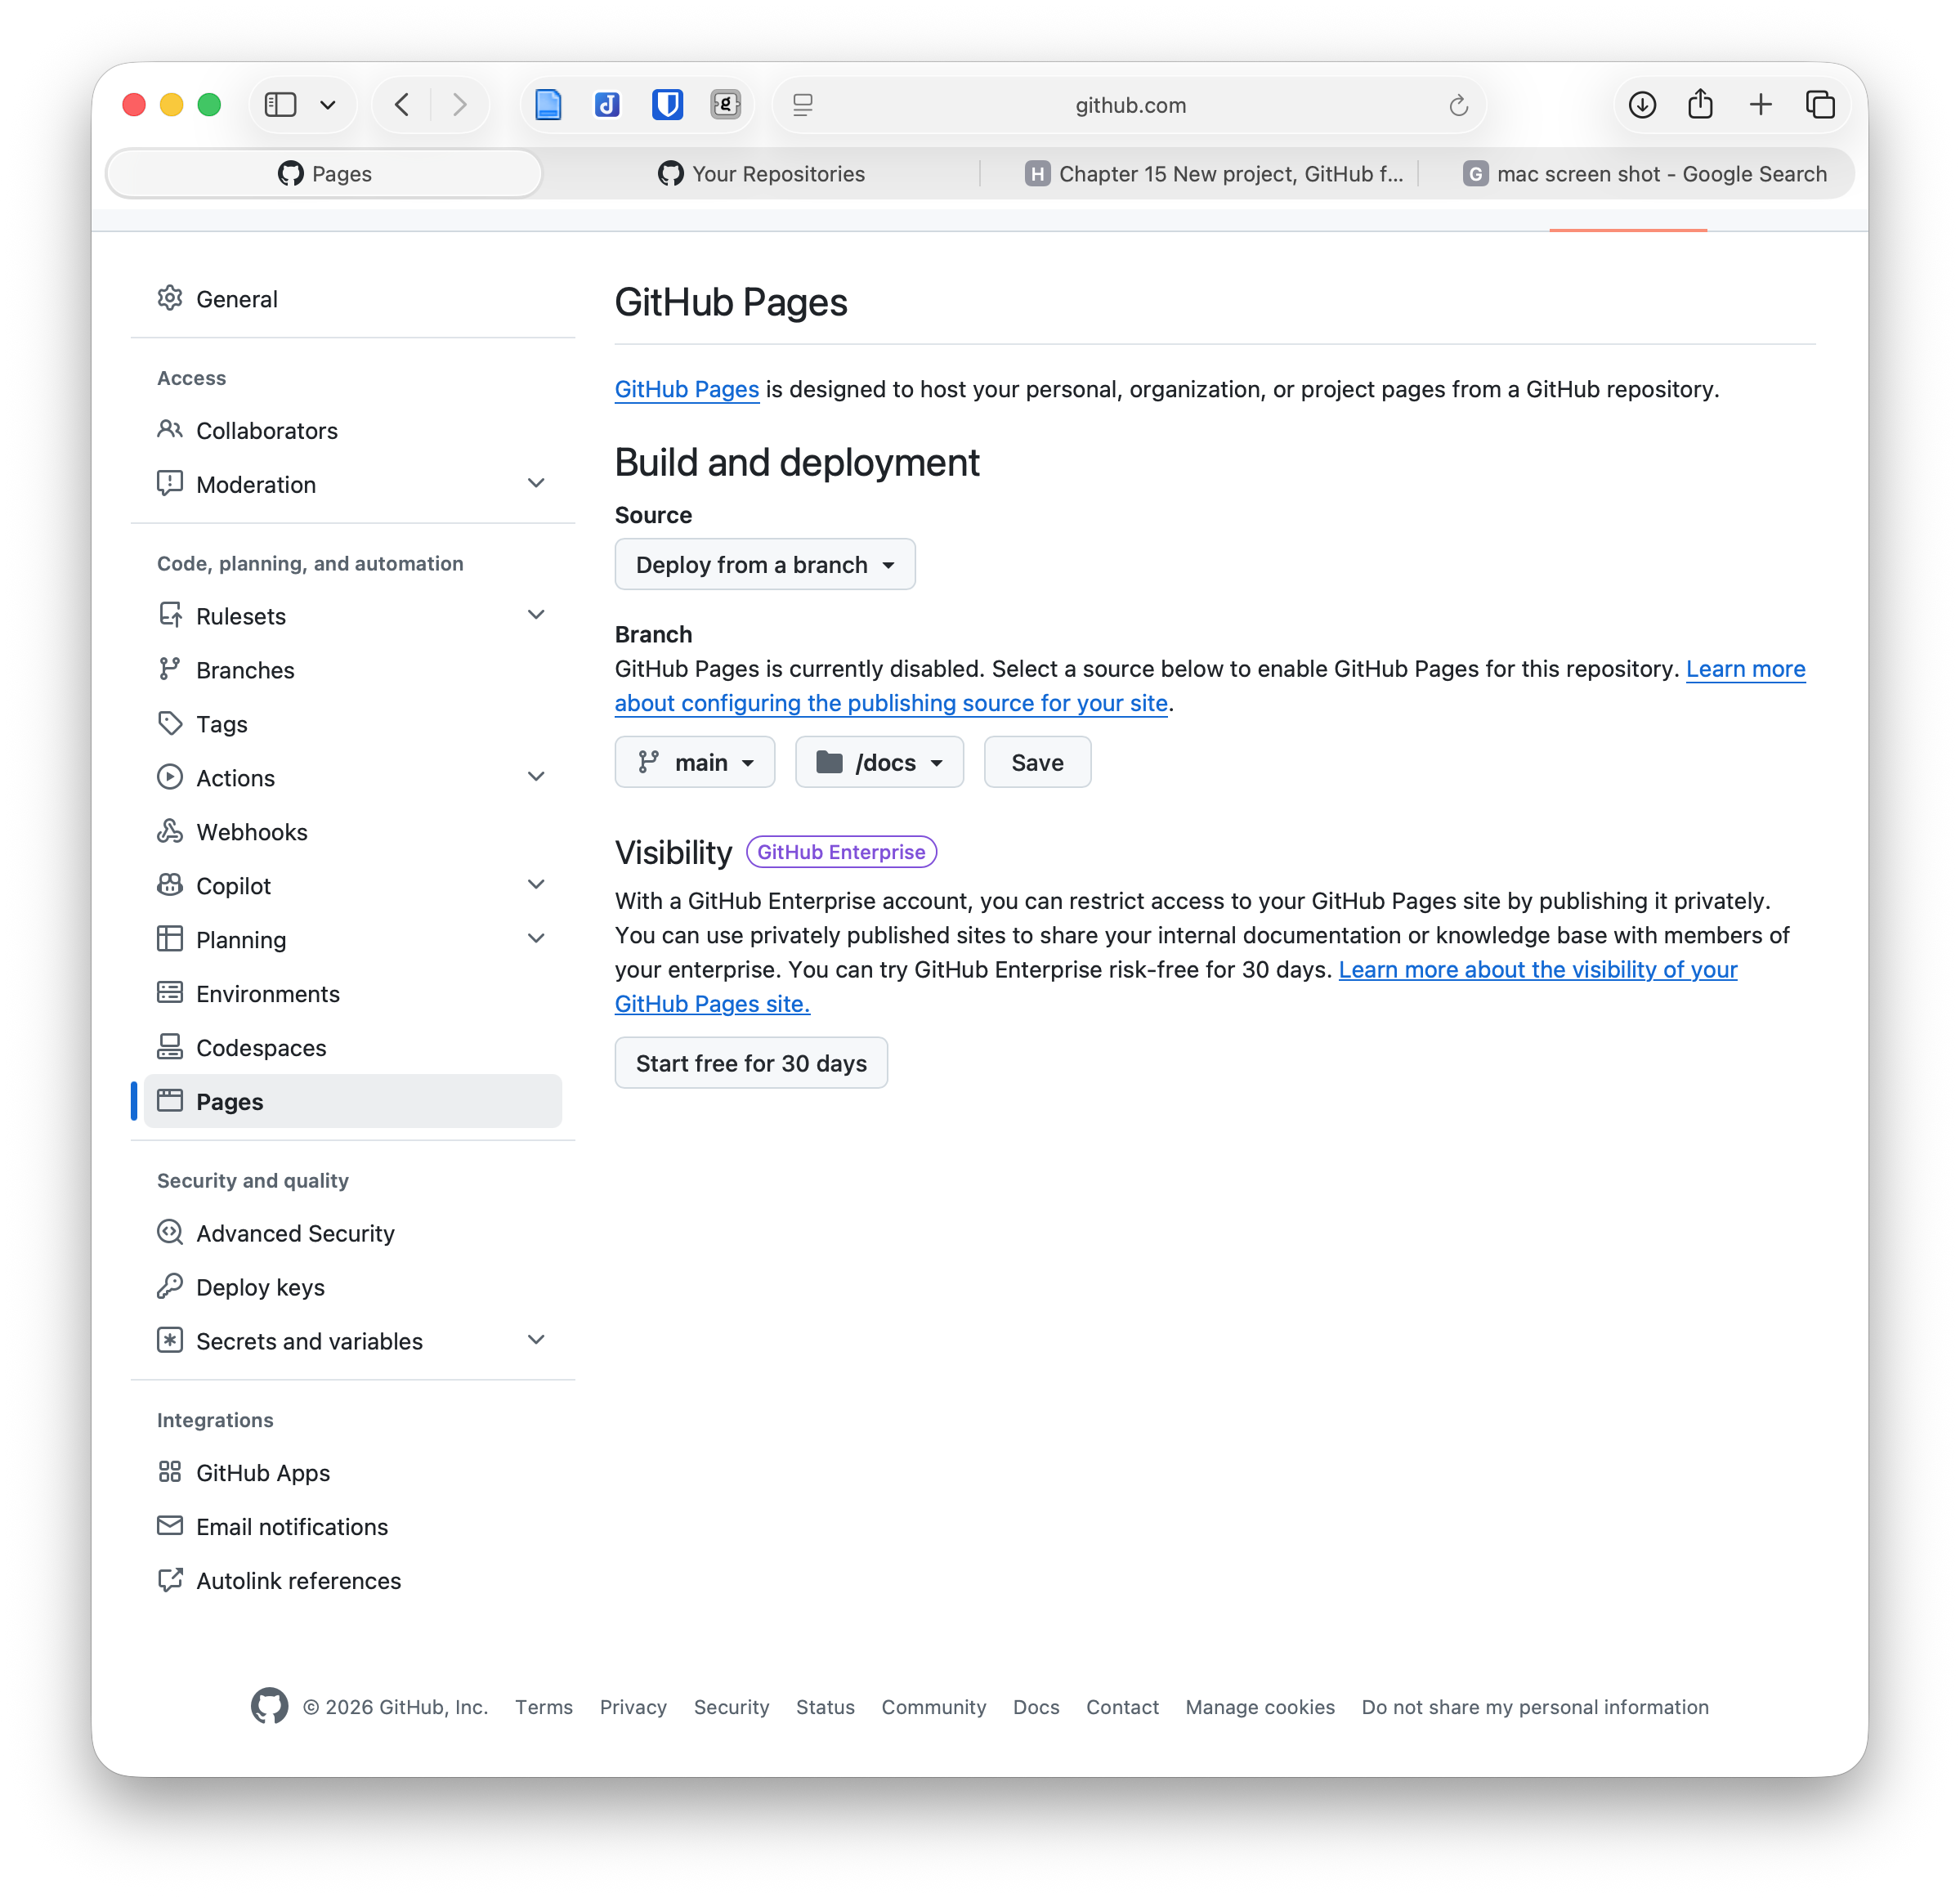
\includegraphics[width=0.6\linewidth,height=\textheight,keepaspectratio]{files/github-pages-point-to-docs.png}

}

\caption{\label{fig-github-pages-point-to-docs}github-pages-point-to-docs}

\end{figure}%

\subsubsection{Check the live site}\label{check-the-live-site}

GitHub will build and deploy within a minute or two. Your site will be
live at https://.github.io//. Any time you edit content, re-run quarto
render, commit the updated docs/ folder, and push --- no separate
publish command needed with this method.

\begin{itemize}
\tightlist
\item
  You can see that the book has now deployed to a live webpage in the
  Deployments column of the GitHub view of your repository.
\end{itemize}

\begin{figure}

\centering{

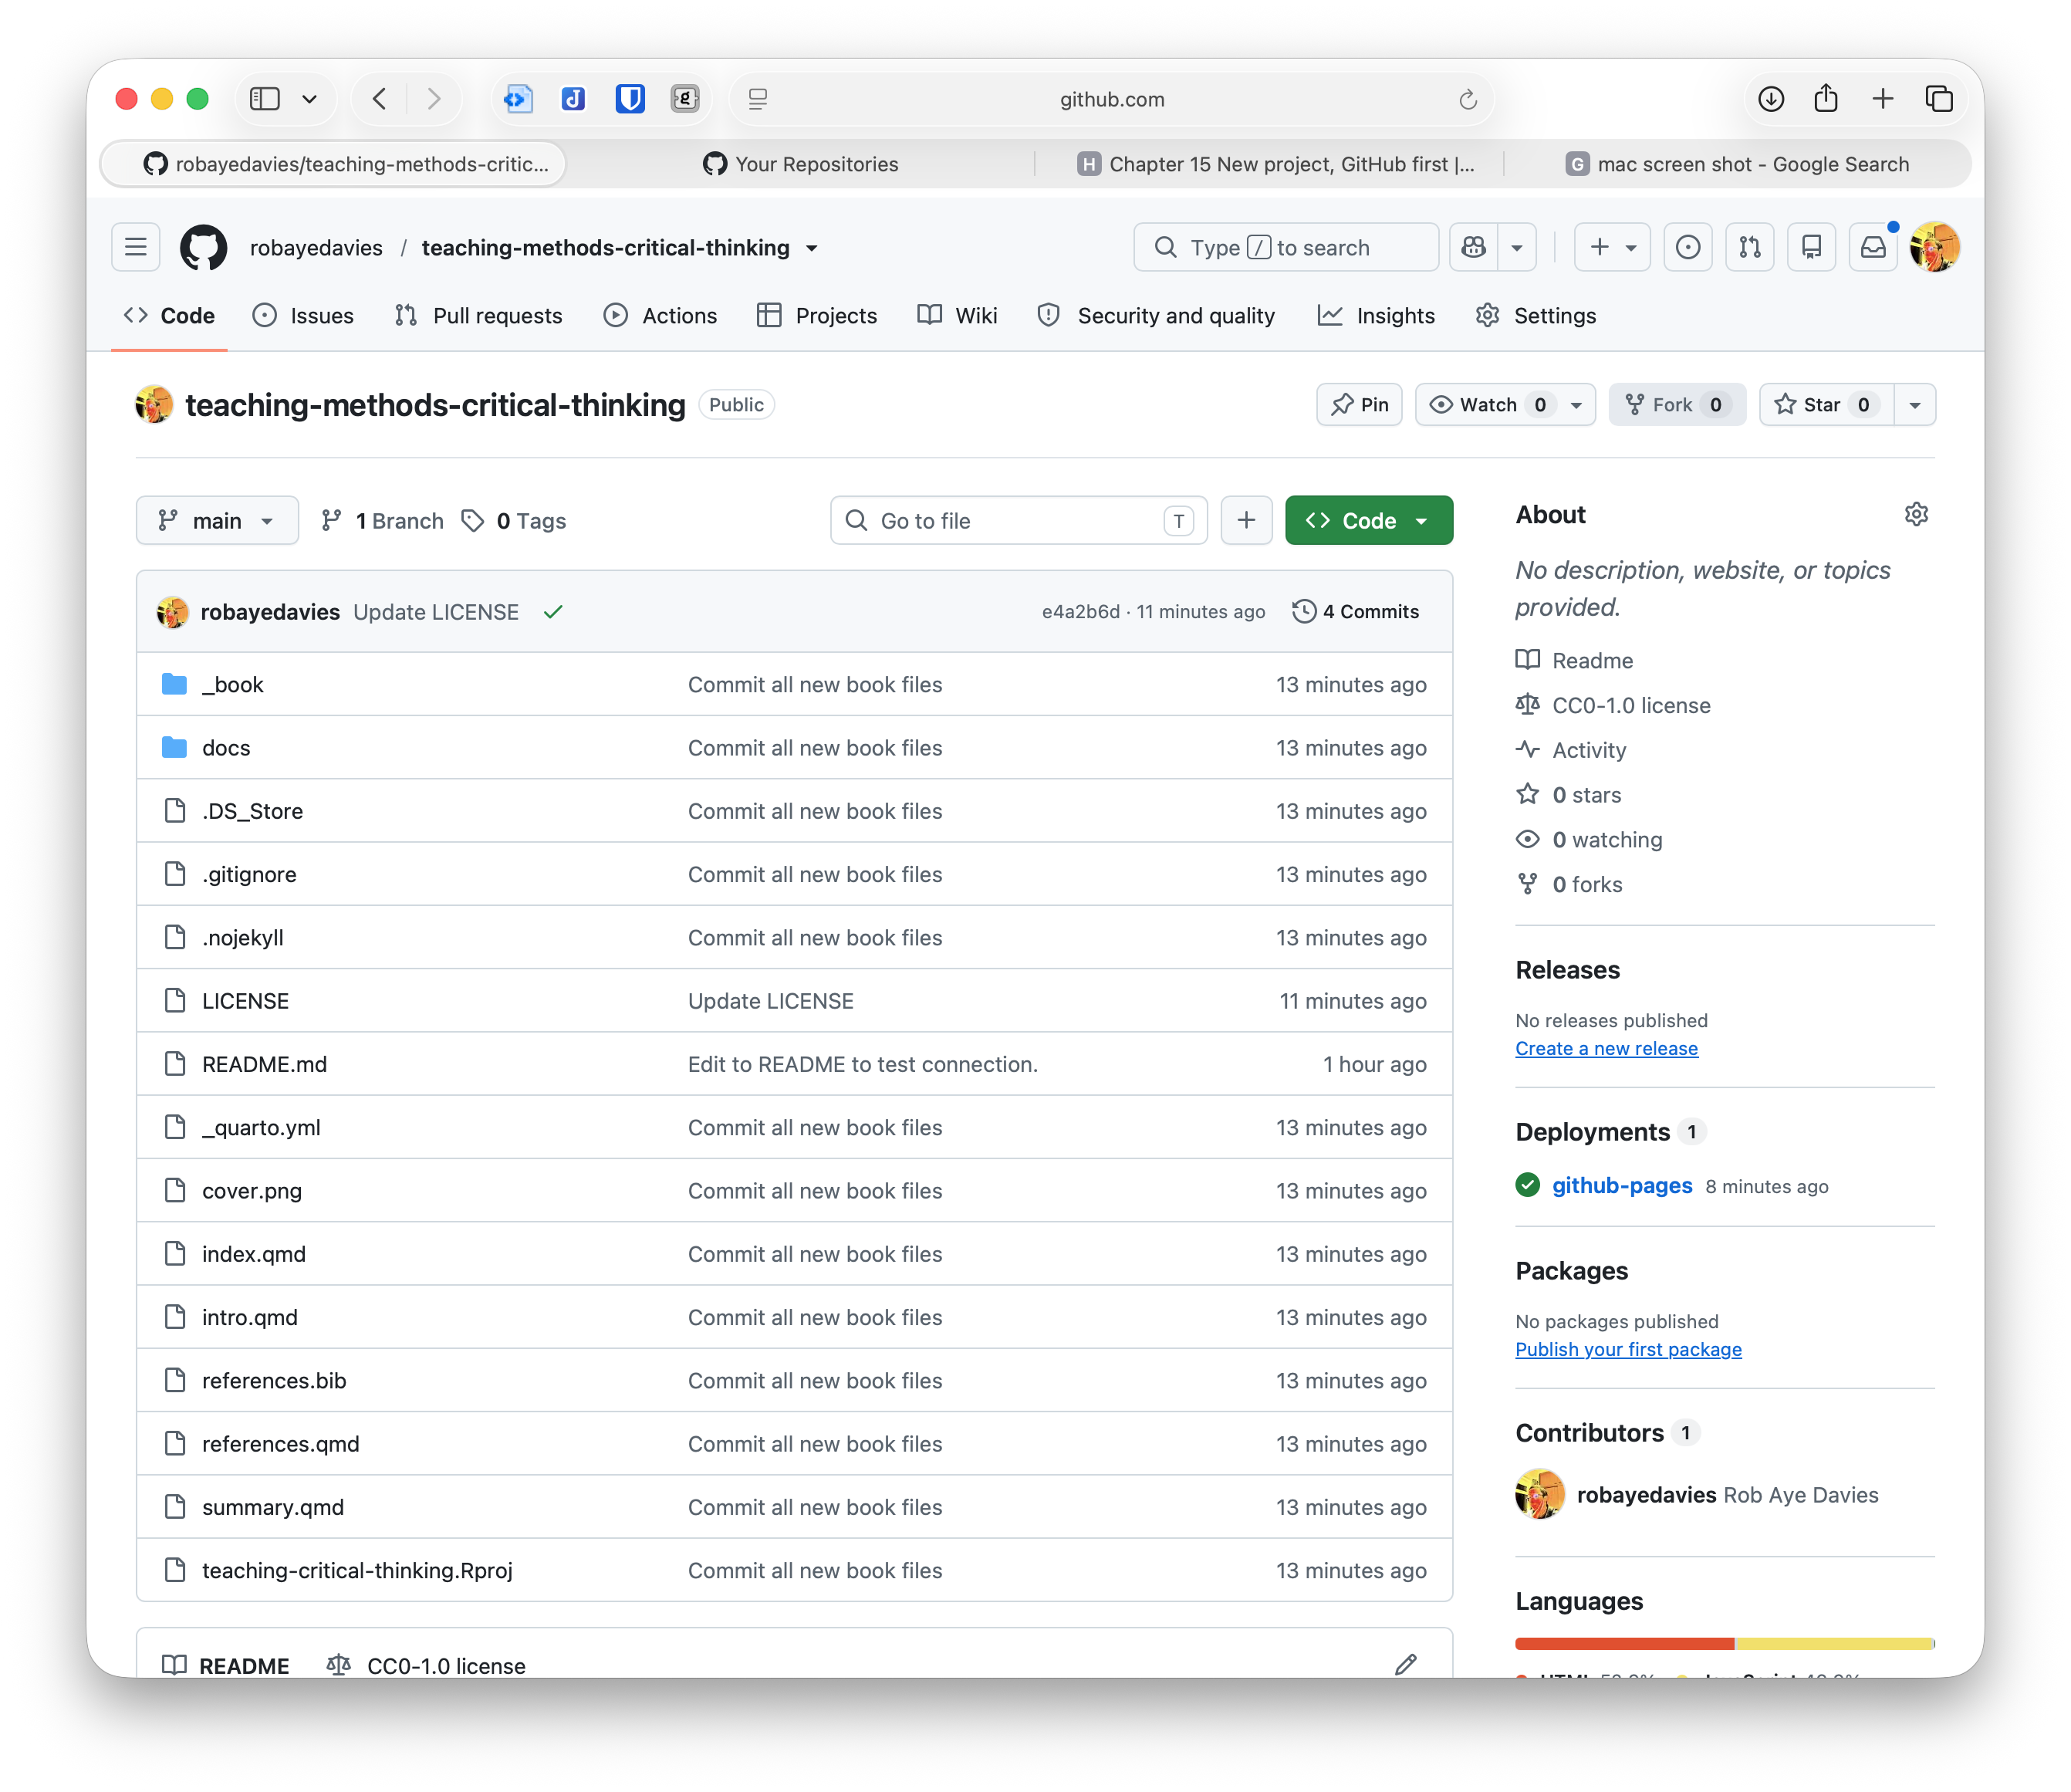
\includegraphics[width=0.6\linewidth,height=\textheight,keepaspectratio]{files/github-deployment.png}

}

\caption{\label{fig-github-deployment}github-deployment}

\end{figure}%

\begin{itemize}
\tightlist
\item
  If you click on the button \texttt{github-pages}, you get taken to a
  deployment information window:
\end{itemize}

\begin{figure}

\centering{

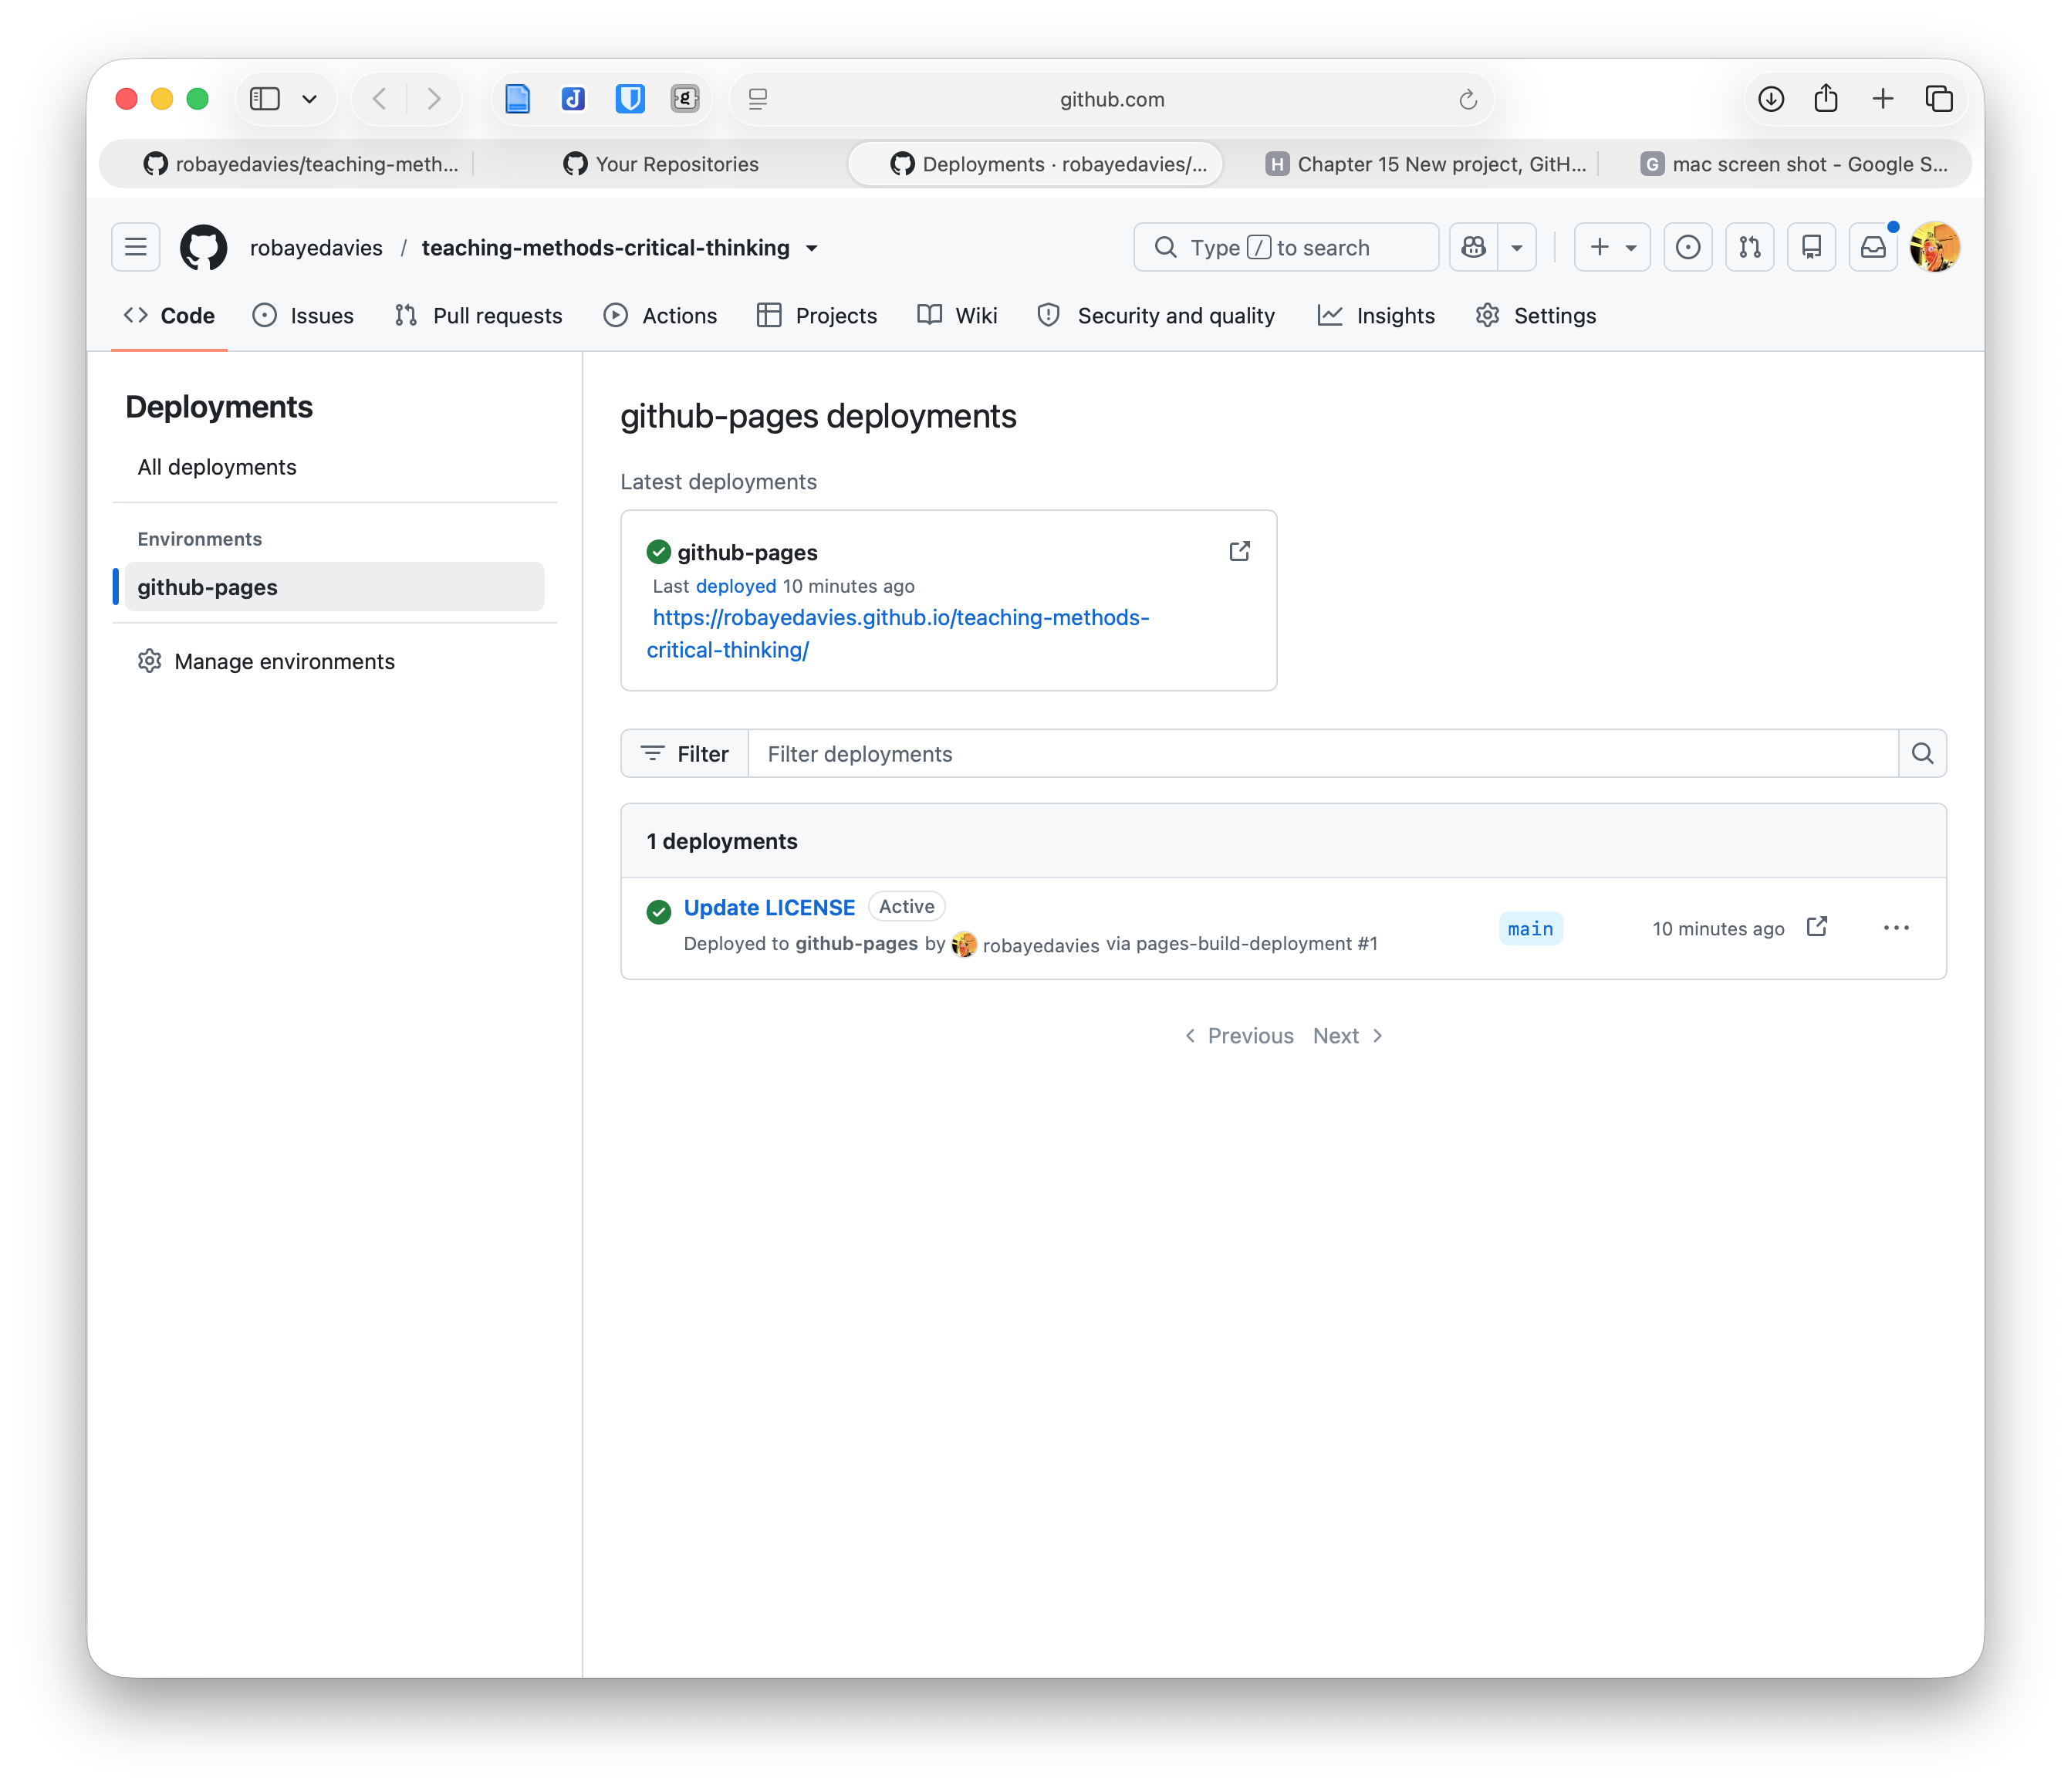
\includegraphics[width=0.6\linewidth,height=\textheight,keepaspectratio]{files/github-deployment-info.png}

}

\caption{\label{fig-github-deployment-infot}github-deployment-info}

\end{figure}%

\begin{itemize}
\tightlist
\item
  where you can see a link (shown as the URL) to the now live webpage:
\end{itemize}

\url{https://robayedavies.github.io/teaching-methods-critical-thinking/}

Let's move next to write or to make edits to some content.

\bookmarksetup{startatroot}

\chapter{Quarto workflow overview}\label{quarto-workflow-overview}

\section{The typical workflow: locating where you
work}\label{the-typical-workflow-locating-where-you-work}

Mostly, we would expect to work to write or to make edits to content for
a book like this book in the following workflow.

\begin{itemize}
\tightlist
\item
  We could but we typically will not make edits to files in the
  repository through GitHub. Notice that the repository view shows us
  the files in the repository folder.
\end{itemize}

\begin{figure}

\centering{

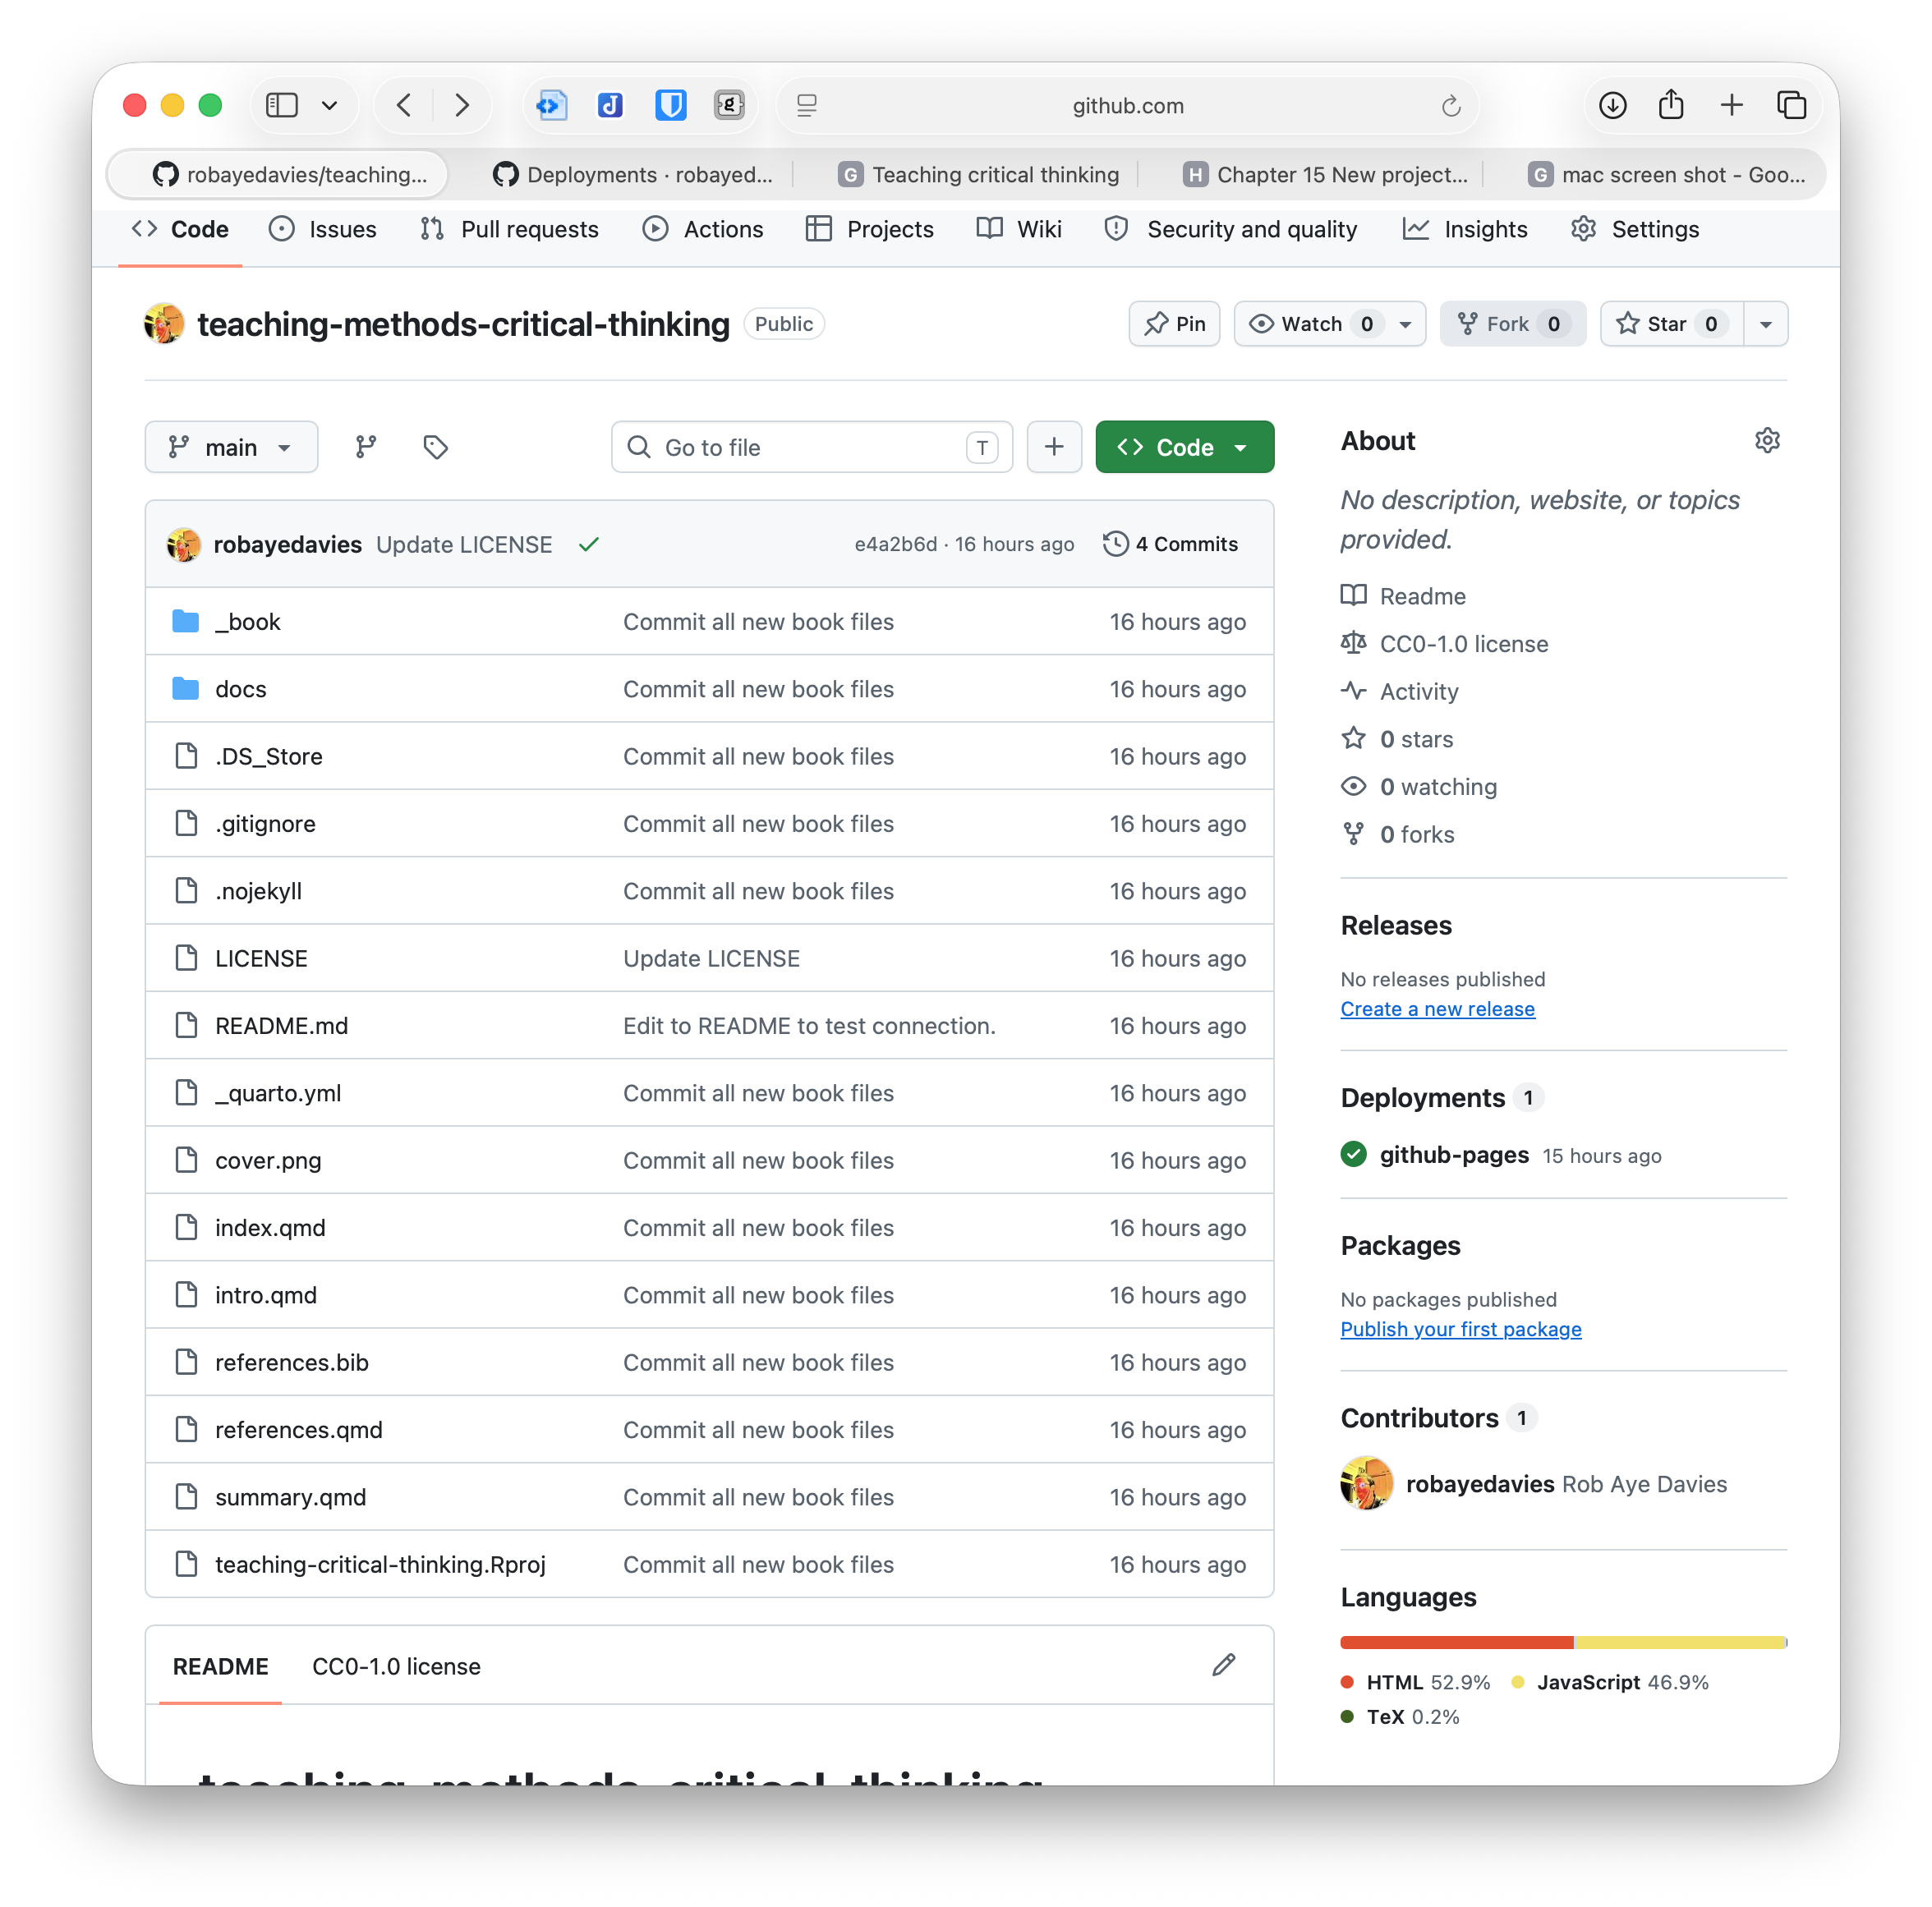
\includegraphics[width=0.6\linewidth,height=\textheight,keepaspectratio]{files/github-repository-information-file-view.png}

}

\caption{\label{fig-github-repository-information-file-view}github-repository-information-file-view}

\end{figure}%

If you click on the files e.g.~the \texttt{references.bib} file then you
can see the file contents and a pencil at the top of the file view
window. If you clicked on the pencil, you could edit the file contents
directly through the GitHub web interface.

\begin{figure}

\centering{

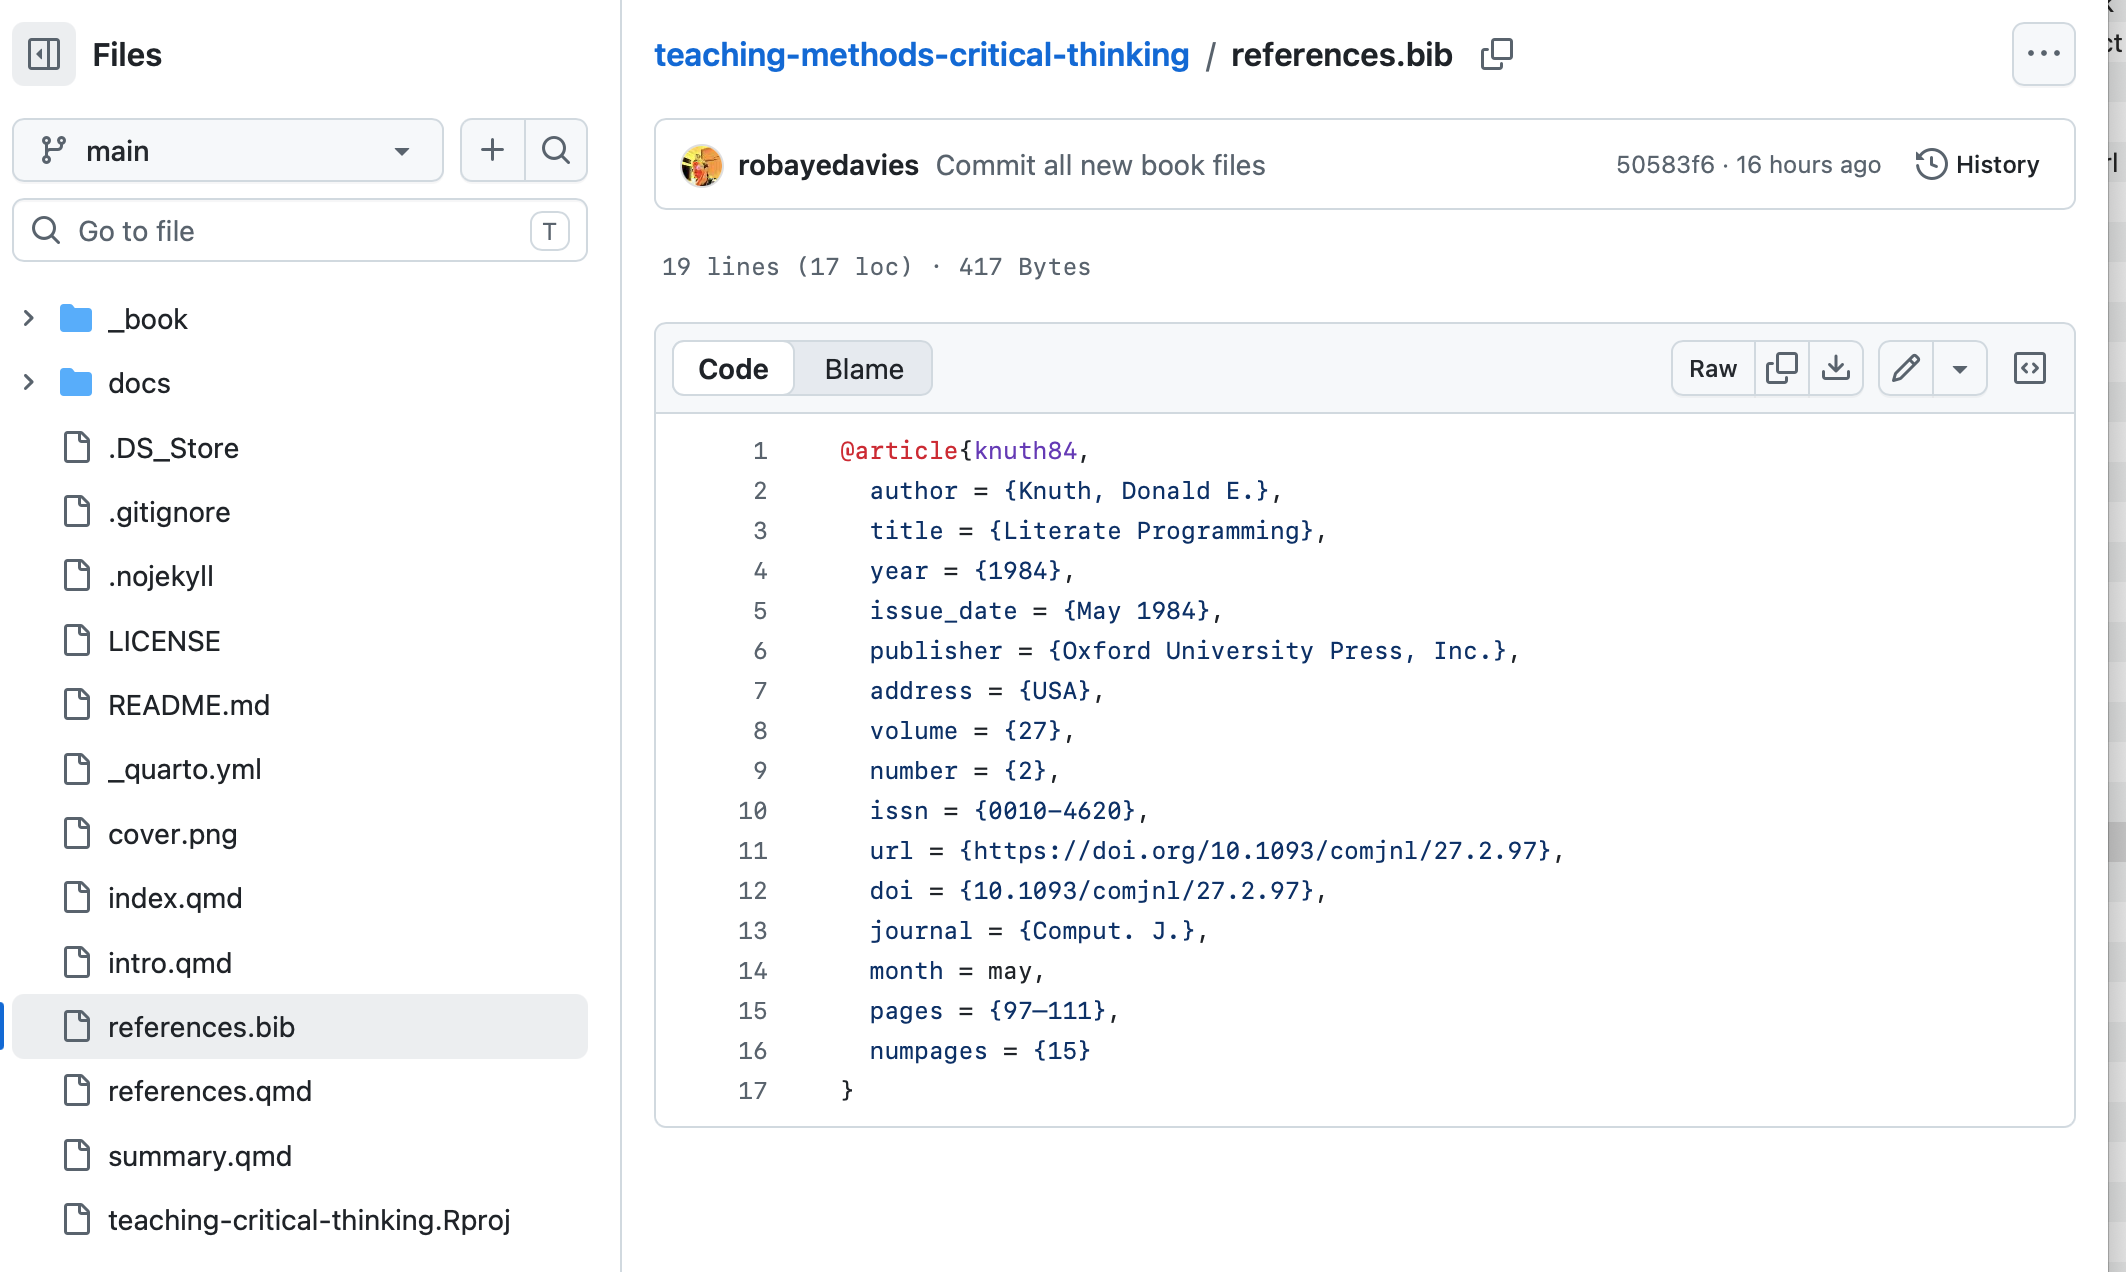
\includegraphics[width=0.6\linewidth,height=\textheight,keepaspectratio]{files/github-repository-information-file-edit-view.png}

}

\caption{\label{fig-github-repository-information-file-edit-view}github-repository-information-file-edit-view}

\end{figure}%

\begin{itemize}
\tightlist
\item
  We are not going to do that.
\end{itemize}

Most of the time, I would expect us to work locally (on our computer):

\begin{itemize}
\tightlist
\item
  with the contents of the local hard drive folder version of our
  project folder;
\item
  writing, or making edits, to those contents or to new content elements
  in the R-Studio IDE (or the new Positron IDE);
\item
  and ultimately pushing those local changes from our computer up to the
  remote repository.
\end{itemize}

In any working session, then, we would begin by opening the project
folder by clicking on it in our file folder window (Finder in Macs).
Here, that means clicking on the
\texttt{teaching-critical-thinking.Rproj} file name.

\begin{figure}

\centering{

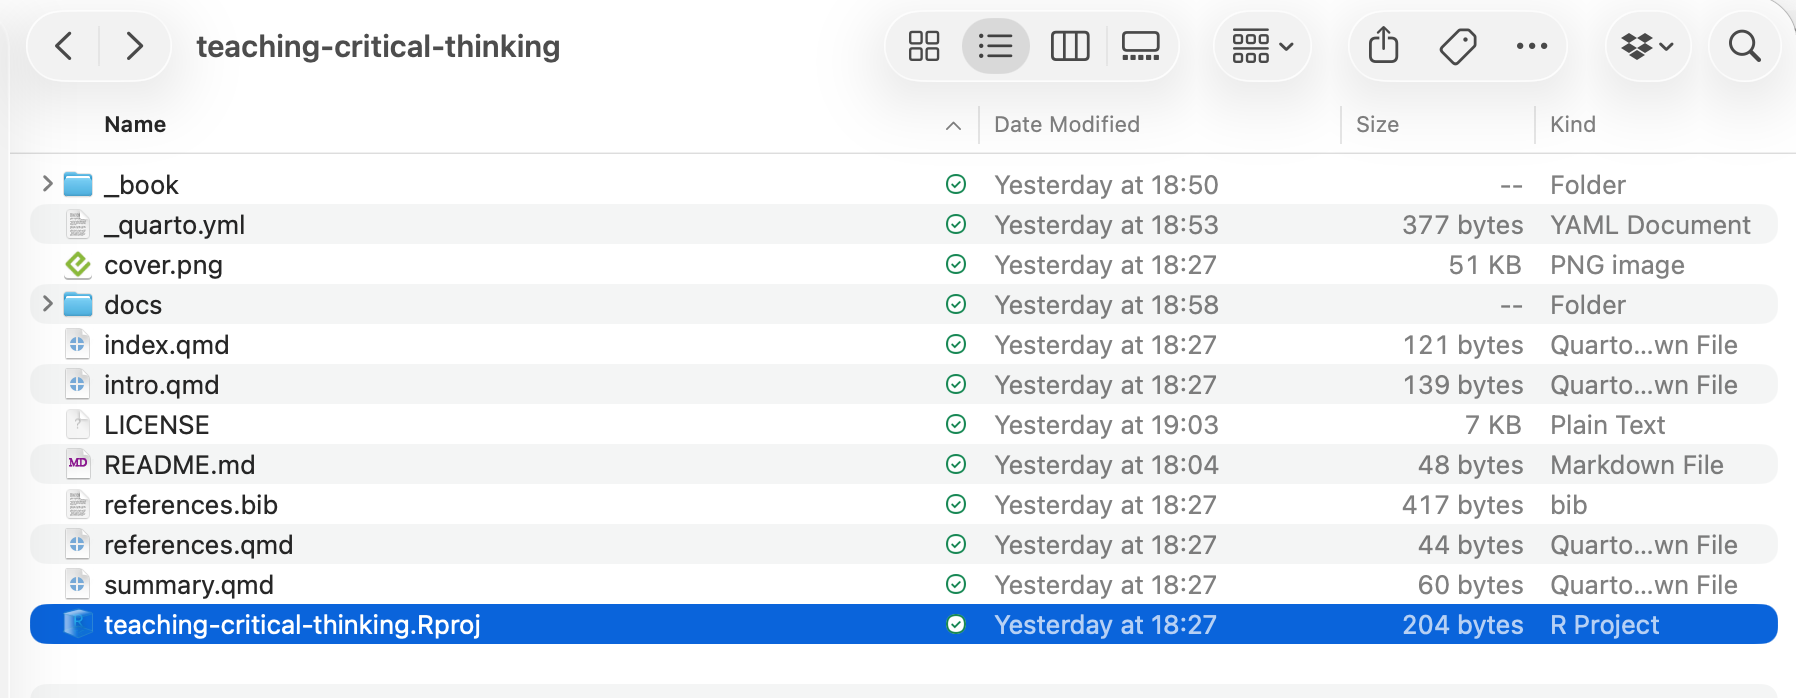
\includegraphics[width=0.6\linewidth,height=\textheight,keepaspectratio]{files/finder-project-folder-rproj.png}

}

\caption{\label{fig-finder-project-folder-rproj}finder-project-folder-rproj}

\end{figure}%

In whatever project you are working on, the workflow to this point will
ensure you have an \texttt{.Rproj} folder file to work with at the top
level of the folder.

\begin{itemize}
\tightlist
\item
  Things are changing but generally a project oriented workflow is the
  recommended practice:
\end{itemize}

\url{https://tidyverse.org/blog/2017/12/workflow-vs-script/}

\begin{itemize}
\tightlist
\item
  See this information on the New Folder from Template workflow in
  Positron (this is a place-holder for thinking about this workflow):
\end{itemize}

\url{https://positron.posit.co/folder-templates.html}

\section{The typical workflow: thinking about the sequence of
actions}\label{the-typical-workflow-thinking-about-the-sequence-of-actions}

Typically, you may proceed as follows: we assume that we are working in
RStudio, in the context of the \texttt{.Rproj} folder for the project.

\begin{itemize}
\tightlist
\item
  I may sensibly begin in the Git window in RStudio (RStudio/Git) by
  clicking on Pull to check if any changes have been made to the project
  following my last action, and to pull down those changes from the
  remote repository to my local version of the repository.
\item
  I create a file or edit a file.
\item
  I save the changes.
\item
  I commit and push the changes from my local to the remote repository.
\item
  Maybe I'll preview the results of the changes.
\item
  I cycle through these changes until I am ready to render.
\item
  I render.
\item
  I push the changed or new files resulting from the render process.
\end{itemize}

\section{Creating or editing content}\label{creating-or-editing-content}

We can think about creating or editing content in terms of multiple
aspects. We can distinguish these aspects though we may not always be
working on all of them:

\begin{itemize}
\tightlist
\item
  Structure -- working with parts, chapters, sections, blocks, divs and
  spans;
\item
  Content -- text, images, computation inline or in code chunks;
\item
  Cross-references -- to other book parts, to chapters, and to sections,
  figures, tables, files and other resources, and links to external
  webpages.
\end{itemize}

Information on book structure is here:

\url{https://quarto.org/docs/books/book-structure.html}

Information on working with markdown in Quarto to create or edit content
is here:

\url{https://quarto.org/docs/authoring/markdown-basics.html\#sec-divs-and-spans}

Information on working with R is here:

\url{https://quarto.org/docs/computations/r.html}

Information on cross-references is here:

\url{https://quarto.org/docs/computations/r.html}

\bookmarksetup{startatroot}

\chapter{Introduction working with
Quarto}\label{introduction-working-with-quarto}

\section{Organizing a book into parts and
chapters}\label{organizing-a-book-into-parts-and-chapters}

I have a rough idea in mind for a draft structure of parts and chapters.
The book will be split into two parts:

\begin{itemize}
\tightlist
\item
  Content for teaching and learning, focused on critical thinking;
\item
  Self-documenting writing and producing the book in Quarto.
\end{itemize}

I'll edit the yaml to add in the parts I'm thinking about right now.

\begin{itemize}
\tightlist
\item
  I'll also create a bunch of empty .qmd files with the titles of the
  chapters I'm thinking about. This is so that the index process
  associated with the yaml can work without error:
\item
  You create a new .qmd by going to: RStudio/File/New
  File/\texttt{Quarto\ Document\ ...} -- and clicking on the
  \texttt{Create\ Empty\ Document} at the bottom of the dialogue box.
\item
  When you do this, each new empty file will be created with a minimal
  yaml section e.g.:
\end{itemize}

\begin{Shaded}
\begin{Highlighting}[]
\SpecialCharTok{{-}{-}{-}}
\NormalTok{title}\SpecialCharTok{:} \StringTok{"[quarto file name.qmd]"}
\NormalTok{editor}\SpecialCharTok{:}\NormalTok{ visual}
\SpecialCharTok{{-}{-}{-}}
\end{Highlighting}
\end{Shaded}

\begin{itemize}
\item
  To reduce redundancy, I'm going to delete the \texttt{editor:\ visual}
  bit from each file. I will add it to \texttt{\_quarto.yml} so that
  this property is then inherited by every book chapter .qmd.
\item
  I also need to rename the dummy files created when I first created the
  book. I can do this directly in the file folder.
\end{itemize}

\texttt{intro.qmd} -\textgreater{} \texttt{introduction.qmd}
\texttt{summary.qmd} -\textgreater{} \texttt{conclusions.qmd}

The \texttt{\_quarto.yml} now looks like this:

\begin{Shaded}
\begin{Highlighting}[]
\NormalTok{project}\SpecialCharTok{:}
\NormalTok{  type}\SpecialCharTok{:}\NormalTok{ book}
\NormalTok{  output}\SpecialCharTok{{-}}\NormalTok{dir}\SpecialCharTok{:}\NormalTok{ docs}

\NormalTok{book}\SpecialCharTok{:}
\NormalTok{  title}\SpecialCharTok{:} \StringTok{"Teaching critical thinking"}
\NormalTok{  author}\SpecialCharTok{:} \StringTok{"Rob Davies"}
\NormalTok{  date}\SpecialCharTok{:} \StringTok{"9/15/2026"}
\NormalTok{  chapters}\SpecialCharTok{:}

    \SpecialCharTok{{-}}\NormalTok{ index.qmd}

    \SpecialCharTok{{-}}\NormalTok{ part}\SpecialCharTok{:} \StringTok{"Critical thinking"}

    \SpecialCharTok{{-}}\NormalTok{ introduction.qmd}

    \SpecialCharTok{{-}}\NormalTok{ how}\SpecialCharTok{{-}}\NormalTok{science}\SpecialCharTok{{-}}\NormalTok{works.qmd}
    \SpecialCharTok{{-}}\NormalTok{ what}\SpecialCharTok{{-}}\NormalTok{is}\SpecialCharTok{{-}}\NormalTok{theory.qmd}
    \SpecialCharTok{{-}}\NormalTok{ evaluating}\SpecialCharTok{{-}}\NormalTok{evidence.qmd}
    \SpecialCharTok{{-}}\NormalTok{ lying}\SpecialCharTok{{-}}\NormalTok{cheating.qmd}
    \SpecialCharTok{{-}}\NormalTok{ criticality}\SpecialCharTok{{-}}\ControlFlowTok{in}\SpecialCharTok{{-}}\NormalTok{writing.qmd}
    \SpecialCharTok{{-}}\NormalTok{ criticality}\SpecialCharTok{{-}}\ControlFlowTok{in}\SpecialCharTok{{-}}\NormalTok{visualization.qmd}
    \SpecialCharTok{{-}}\NormalTok{ critical}\SpecialCharTok{{-}}\NormalTok{citation}\SpecialCharTok{{-}}\NormalTok{practice.qmd}
    \SpecialCharTok{{-}}\NormalTok{ subjectivity}\SpecialCharTok{{-}}\NormalTok{objectivity}\SpecialCharTok{{-}}\NormalTok{virtues.qmd}

    \SpecialCharTok{{-}}\NormalTok{ conclusions.qmd    }
    
    \SpecialCharTok{{-}}\NormalTok{ part}\SpecialCharTok{:} \StringTok{"Quarto"}

    \SpecialCharTok{{-}}\NormalTok{ set}\SpecialCharTok{{-}}\NormalTok{up}\SpecialCharTok{{-}}\NormalTok{book.qmd}
    \SpecialCharTok{{-}}\NormalTok{ workflow}\SpecialCharTok{{-}}\NormalTok{overview.qmd    }
    \SpecialCharTok{{-}}\NormalTok{ markdown}\SpecialCharTok{{-}}\NormalTok{basics.qmd}

    \SpecialCharTok{{-}}\NormalTok{ part}\SpecialCharTok{:} \StringTok{"References"}

    \SpecialCharTok{{-}}\NormalTok{ references.qmd}

\NormalTok{bibliography}\SpecialCharTok{:}\NormalTok{ references.bib}

\NormalTok{editor}\SpecialCharTok{:}\NormalTok{ visual}

\NormalTok{format}\SpecialCharTok{:}
\NormalTok{  html}\SpecialCharTok{:}
\NormalTok{    theme}\SpecialCharTok{:}
      \SpecialCharTok{{-}}\NormalTok{ cosmo}
      \SpecialCharTok{{-}}\NormalTok{ brand}
\NormalTok{  pdf}\SpecialCharTok{:}
\NormalTok{    documentclass}\SpecialCharTok{:}\NormalTok{ scrreprt}
\end{Highlighting}
\end{Shaded}

\begin{itemize}
\item
  And the RStudio window shows the new files in both the \texttt{Files}
  sub window or tab, and in the \texttt{Git} tab.
\item
  I commit the changes with the message: Set up book structure, edits to
  \texttt{\_quarto.yml} and create empty .qmd files to hold content for
  new chapters.
\item
  I check the preview in terminal with \texttt{quarto\ preview}. Looks
  good.
\item
  I render the book with \texttt{quarto\ render}.
\end{itemize}

The process of rendering changes the contents of the folder. We see the
creation of new .html files, corresponding to the new chapters. We see
deletion of the html files corresponding to the .qmd files I renamed.

\begin{figure}

\centering{

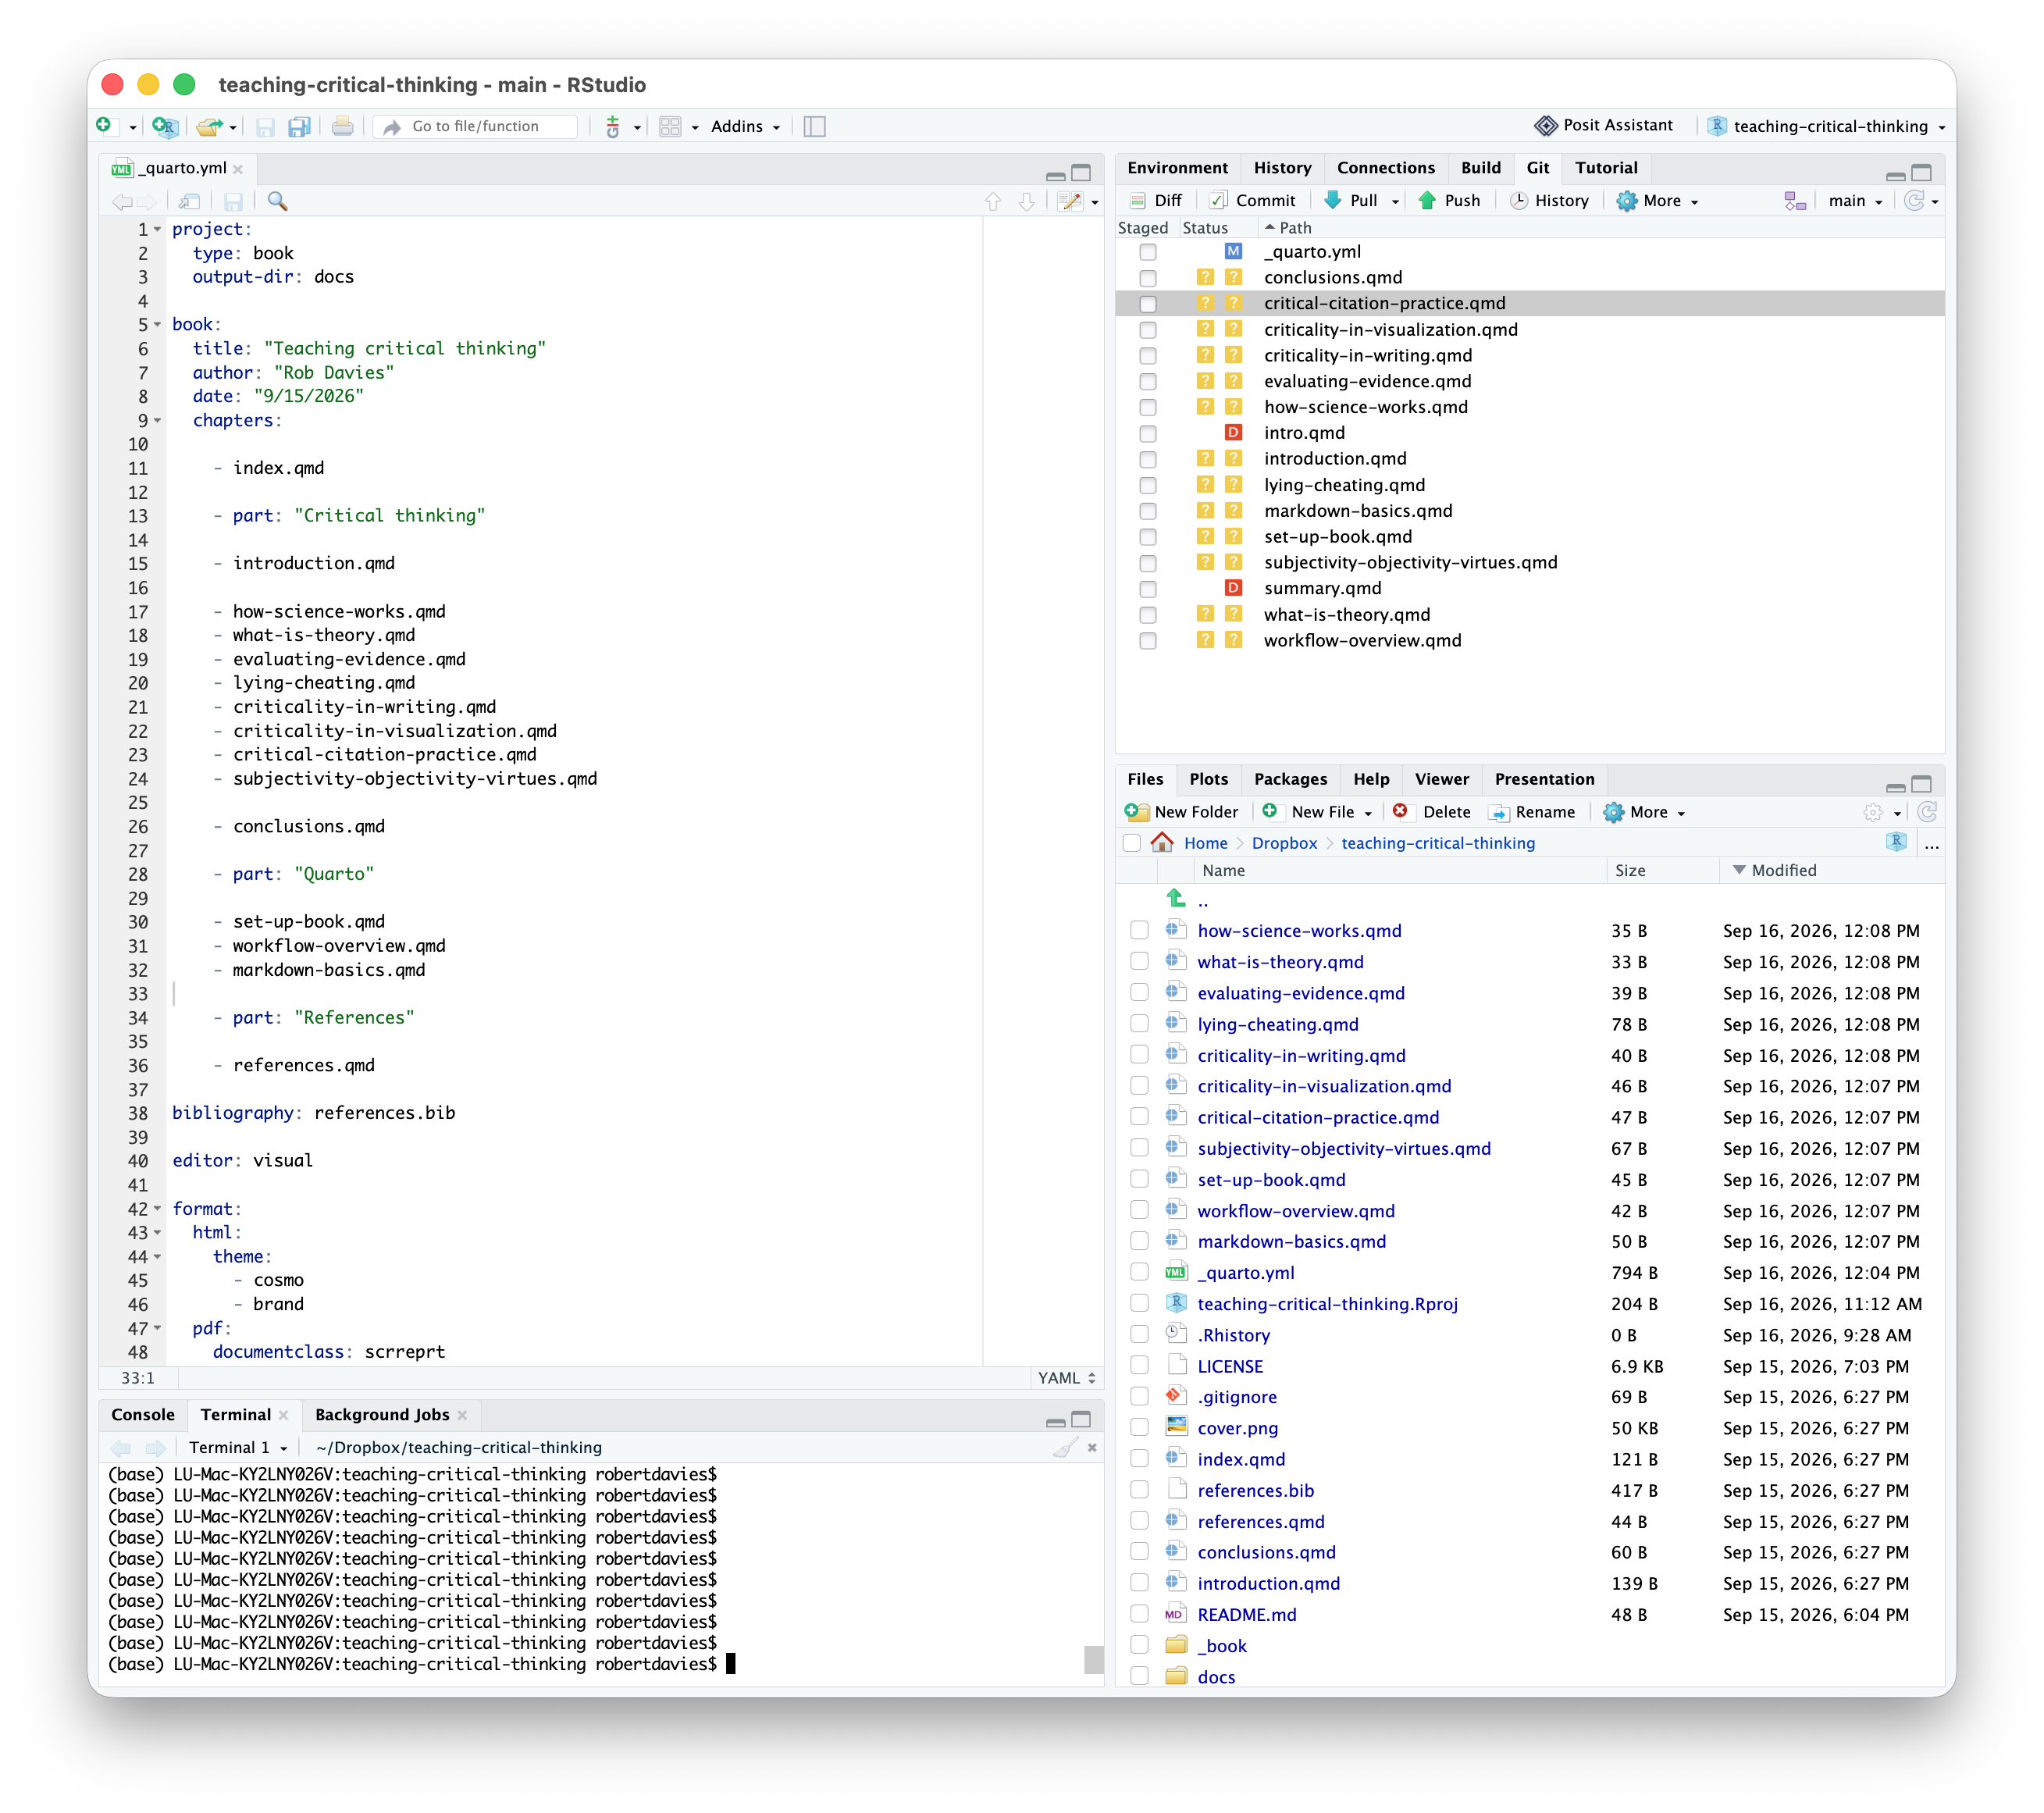
\includegraphics[width=0.6\linewidth,height=\textheight,keepaspectratio]{files/rstudio-edits-changes-git-files.png}

}

\caption{\label{fig-rstudio-edits-changes-git-files}rstudio-edits-changes-git-files}

\end{figure}%

\begin{itemize}
\item
  I first stage the changes: in RStudio/Git under the \texttt{Staged}
  column, click on the check box at the top of the lift, press and hold
  SHIFT, then click on the check box at the bottom of the list, to stage
  all file entries.
\item
  I commit the changes.
\item
  I push the changes. From the moment I push the changes, if I go to the
  web view of my repository, I should be able to see that the deployment
  to GitHub Pages has been refreshed, and the resulting downstream web
  page should represent the revised book structure.
\item
  It does.
\end{itemize}

\begin{figure}

\centering{

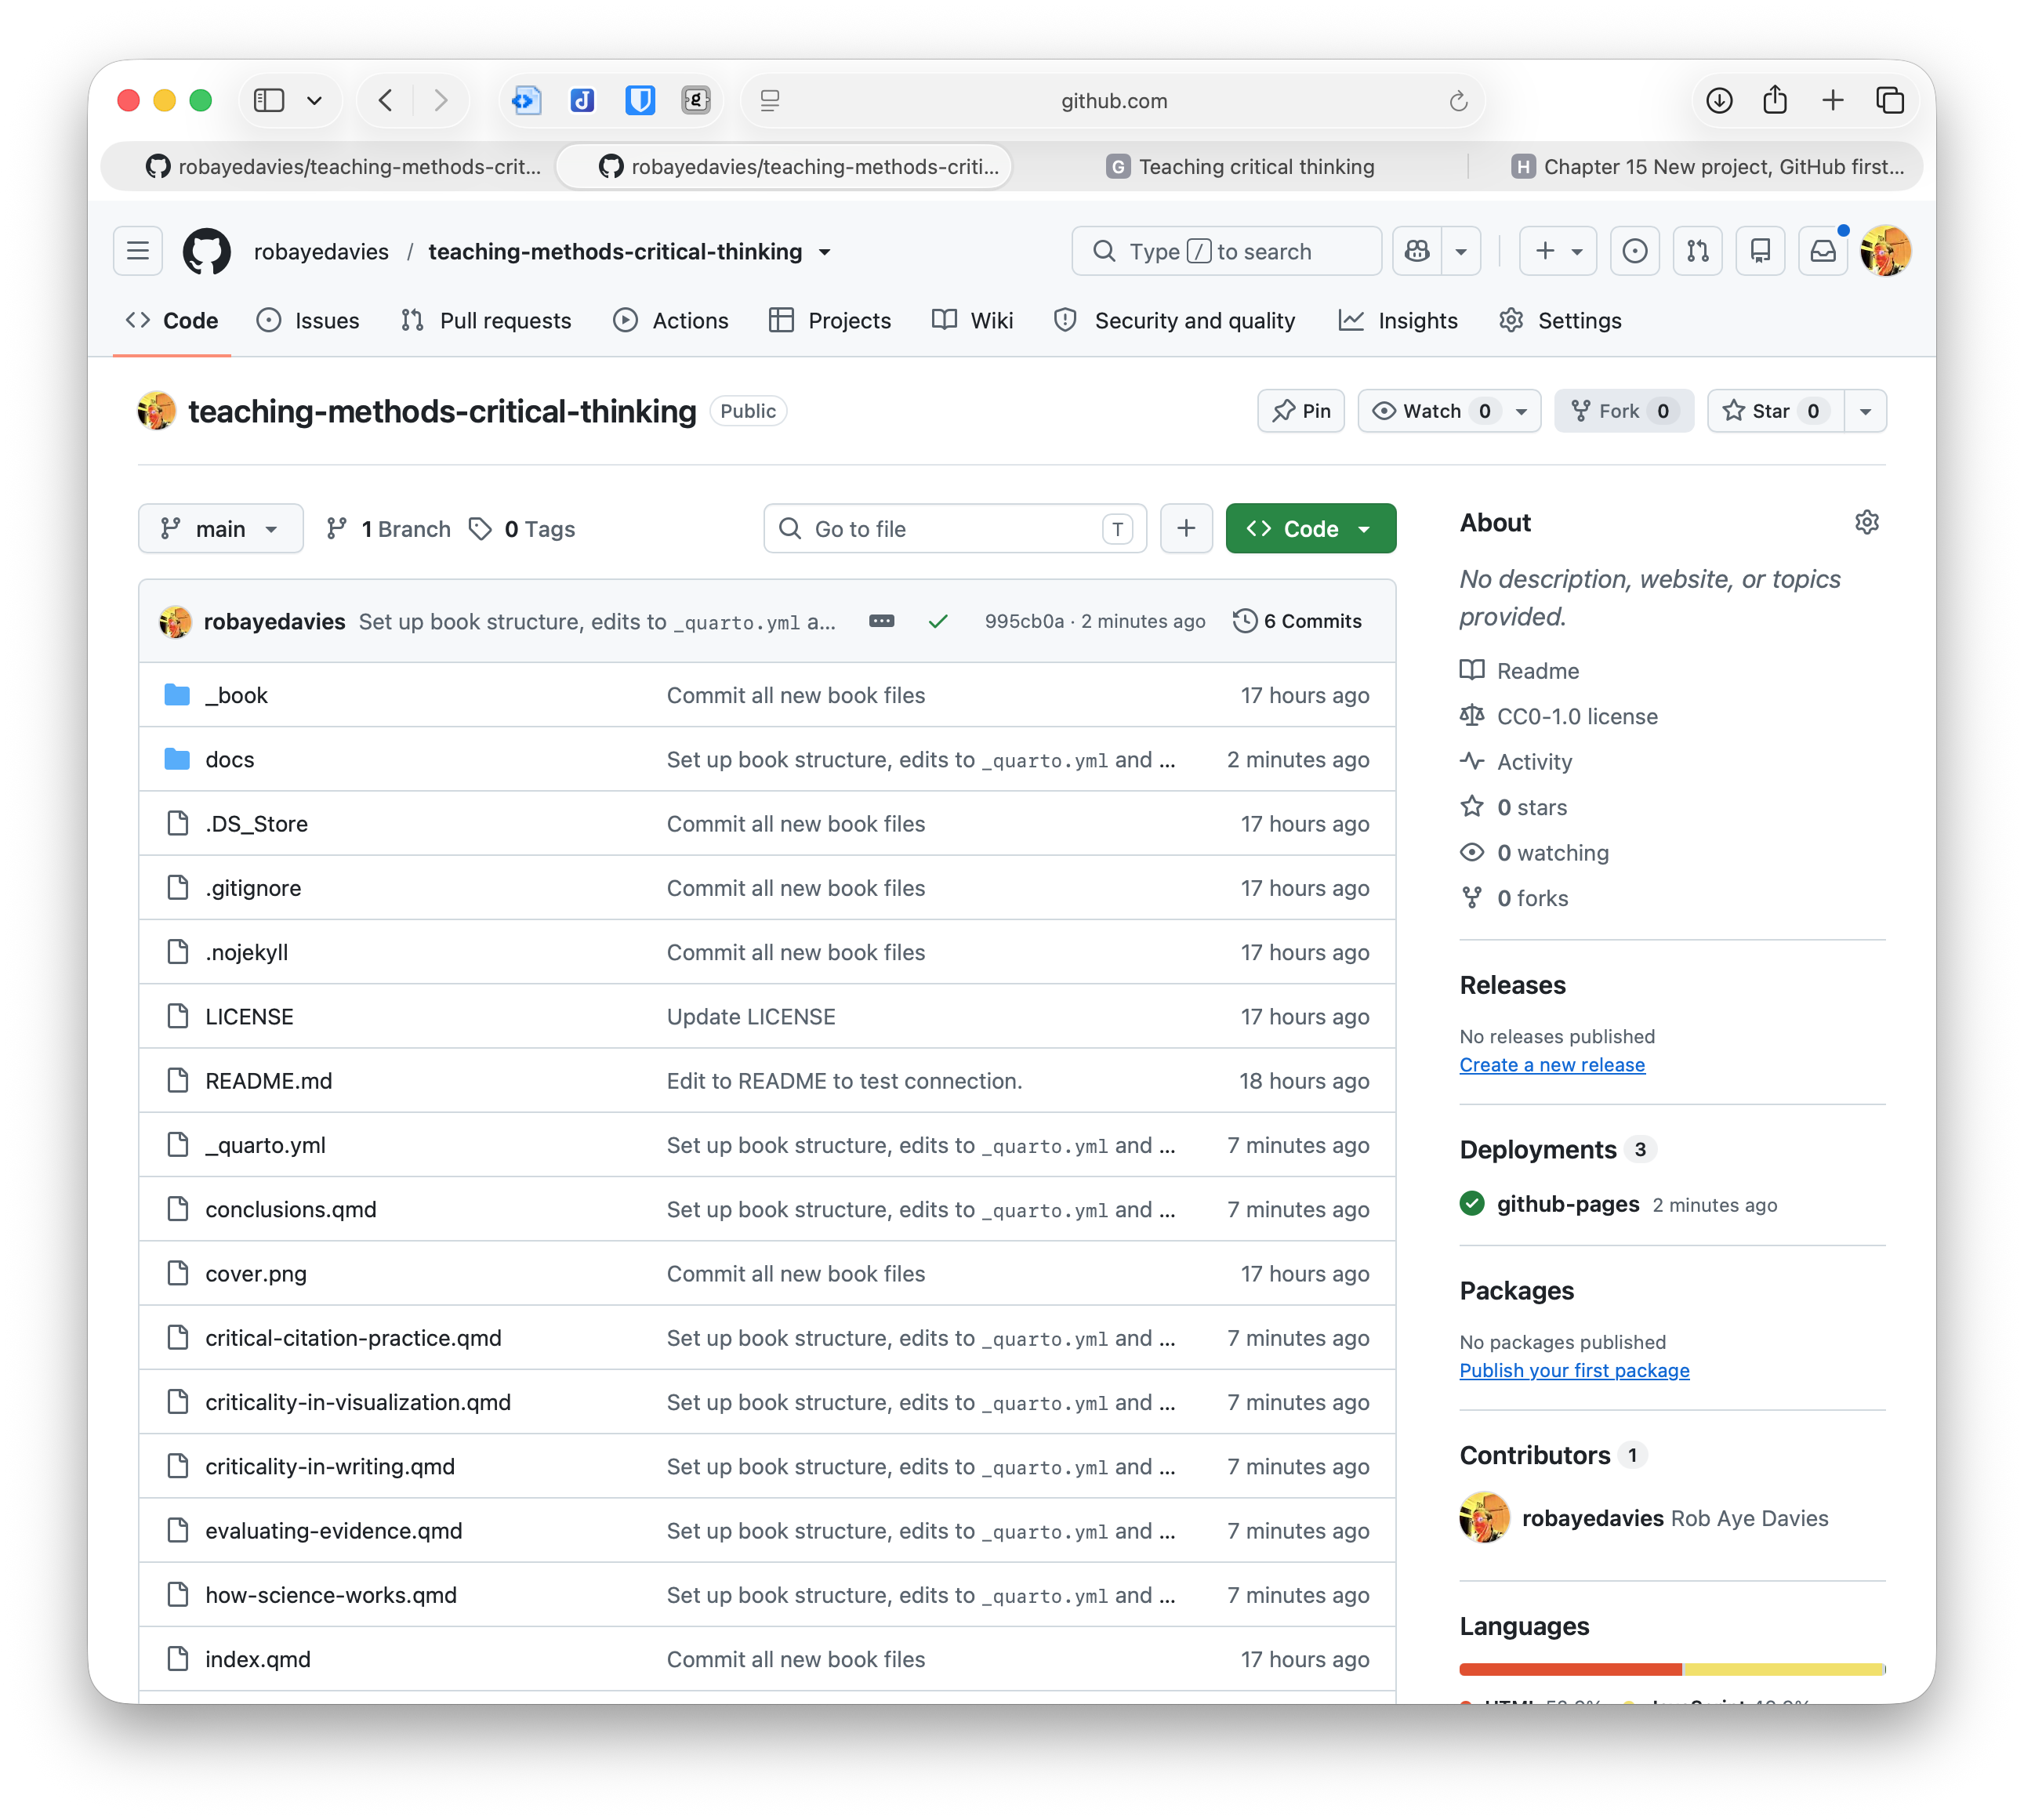
\includegraphics[width=0.6\linewidth,height=\textheight,keepaspectratio]{files/github-repo-pages-deployment-update.png}

}

\caption{\label{fig-github-repo-pages-deployment-update}github-repo-pages-deployment-update}

\end{figure}%

\begin{itemize}
\tightlist
\item
  The output looks ok in Safari:
\end{itemize}

\begin{figure}

\centering{

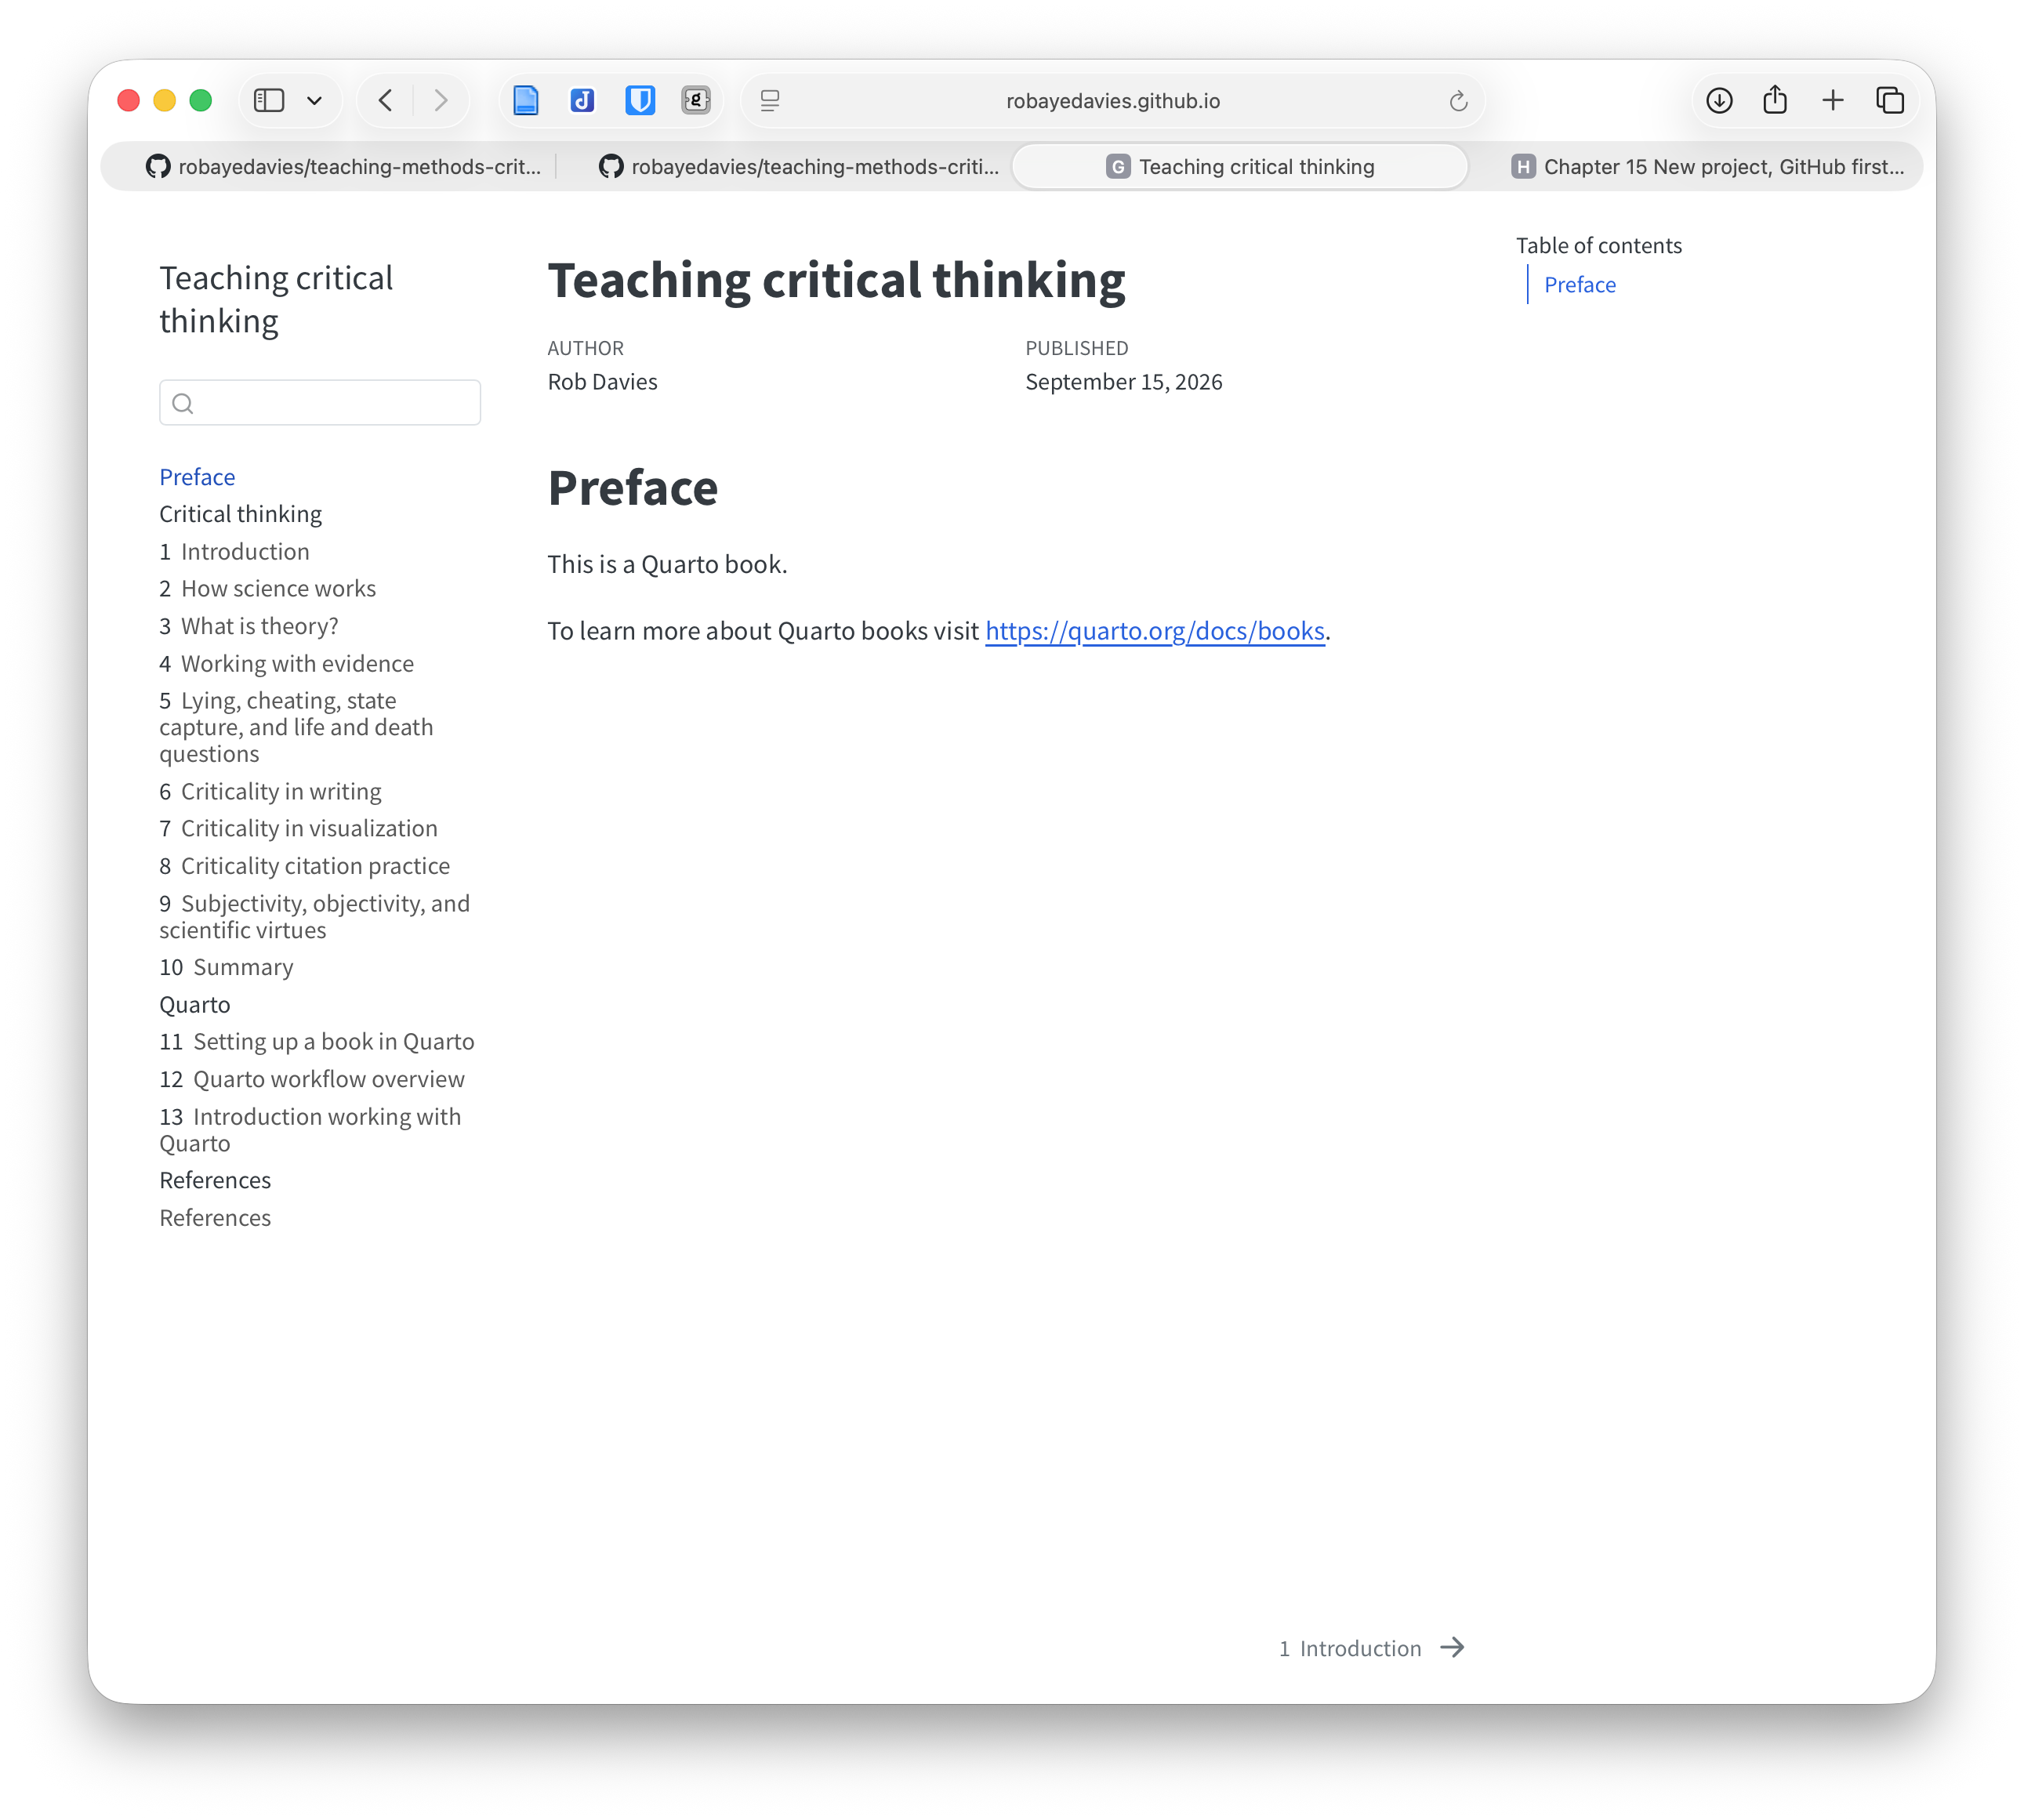
\includegraphics[width=0.6\linewidth,height=\textheight,keepaspectratio]{files/safari-webpage-book-structure-revised.png}

}

\caption{\label{fig-safari-webpage-book-structure-revised}safari-webpage-book-structure-revised}

\end{figure}%

\section{Writing content: adding text, adding sections, adding callout
boxes, and inserting
images}\label{writing-content-adding-text-adding-sections-adding-callout-boxes-and-inserting-images}

\subsection{Adding text}\label{adding-text}

The basics of adding text is covered here:

\url{https://quarto.org/docs/authoring/markdown-basics.html\#links-images}

And most of the time, we are writing stuff like this:

\begin{Shaded}
\begin{Highlighting}[]
\DocumentationTok{\#\#\# Adding text}

\NormalTok{The basics of adding text is covered here}\SpecialCharTok{:} 

\ErrorTok{\textless{}}\NormalTok{https}\SpecialCharTok{:}\ErrorTok{//}\NormalTok{quarto.org}\SpecialCharTok{/}\NormalTok{docs}\SpecialCharTok{/}\NormalTok{authoring}\SpecialCharTok{/}\NormalTok{markdown}\SpecialCharTok{{-}}\NormalTok{basics.html}\CommentTok{\#links{-}images\textgreater{}}
\end{Highlighting}
\end{Shaded}

\subsection{Adding sections}\label{adding-sections}

Most of the time, we are going to divide our text into sections or into
callout boxes.

In Quarto, we use \texttt{\#} marks to identify section headers, varying
the number of \texttt{\#} to indicate the level of section header.

\begin{Shaded}
\begin{Highlighting}[]
\CommentTok{\# Heading 1}

\DocumentationTok{\#\# Heading 2}

\DocumentationTok{\#\#\# Heading 3}

\DocumentationTok{\#\#\#\# Heading 4}

\DocumentationTok{\#\#\#\#\# Heading 5}

\DocumentationTok{\#\#\#\#\#\# Heading 6}
\end{Highlighting}
\end{Shaded}

Quarto will automatically number the sections, and number the sections,
unless we specify otherwise.

We can tell Quarto to do this explicitly in the book yaml or in a
chapter yaml. We can edit the book yaml \texttt{\_quarto.yml} to be
explicit about the behaviour we want.

\begin{Shaded}
\begin{Highlighting}[]
\NormalTok{format}\SpecialCharTok{:}
\NormalTok{  html}\SpecialCharTok{:}
\NormalTok{    theme}\SpecialCharTok{:}
      \SpecialCharTok{{-}}\NormalTok{ cosmo}
      \SpecialCharTok{{-}}\NormalTok{ brand}
\NormalTok{    number}\SpecialCharTok{{-}}\NormalTok{sections}\SpecialCharTok{:}\NormalTok{ true  }
\NormalTok{  pdf}\SpecialCharTok{:}
\NormalTok{    documentclass}\SpecialCharTok{:}\NormalTok{ scrreprt}
\NormalTok{    number}\SpecialCharTok{{-}}\NormalTok{sections}\SpecialCharTok{:}\NormalTok{ true}
\end{Highlighting}
\end{Shaded}

\subsubsection{Cross-referencing
sections}\label{cross-referencing-sections}

Cross references are an important facet of writing Quarto documents. We
can add code to enable automatic referencing of equations, figures,
images, sections and tables.

\url{https://quarto.org/docs/authoring/cross-references.html\#sections}

Let's say we have a section \texttt{\#\#\#\ Inserting\ images}, we can
refer to the section as follows:

\begin{Shaded}
\begin{Highlighting}[]
\DocumentationTok{\#\#\# Inserting images \{\#sec{-}inserting{-}images\}}
\end{Highlighting}
\end{Shaded}

This means that we can then write the code:

\begin{Shaded}
\begin{Highlighting}[]
\SpecialCharTok{@}\NormalTok{sec}\SpecialCharTok{{-}}\NormalTok{inserting}\SpecialCharTok{{-}}\NormalTok{images}
\end{Highlighting}
\end{Shaded}

\begin{itemize}
\tightlist
\item
  to get this: Section~\ref{sec-inserting-images}.
\end{itemize}

\subsection{Adding callout boxes}\label{adding-callout-boxes}

It is often helpful to use callout boxes. We probably ought to be
systematic or consistent about this across chapters (and across the
contributions of different authors).

You can find information about callout boxes here:

\url{https://quarto.org/docs/authoring/cross-references.html\#callouts}

We often want to use one of the following variety of callout boxes --
notice that we can label boxes for cross-referencing:

\begin{Shaded}
\begin{Highlighting}[]
\SpecialCharTok{:::}\NormalTok{ \{}\CommentTok{\#tip{-}example .callout{-}tip\}}
\DocumentationTok{\#\# Cross{-}Referencing a Tip}

\NormalTok{Add an ID starting with }\StringTok{\textasciigrave{}}\AttributeTok{\#tip{-}}\StringTok{\textasciigrave{}}\NormalTok{ to reference a tip.}
\SpecialCharTok{:::}

\NormalTok{See }\SpecialCharTok{@}\NormalTok{tip}\SpecialCharTok{{-}}\NormalTok{example...}
\end{Highlighting}
\end{Shaded}

\begin{tcolorbox}[enhanced jigsaw, arc=.35mm, bottomrule=.15mm, bottomtitle=1mm, breakable, colback=white, colbacktitle=quarto-callout-tip-color!10!white, colframe=quarto-callout-tip-color-frame, coltitle=black, left=2mm, leftrule=.75mm, opacityback=0, opacitybacktitle=0.6, rightrule=.15mm, title=\textcolor{quarto-callout-tip-color}{\faLightbulb}\hspace{0.5em}{Tip \ref*{tip-example}: Cross-Referencing a Tip}, titlerule=0mm, toprule=.15mm, toptitle=1mm]

\quartocallouttip{tip-example} 

Add an ID starting with \texttt{\#tip-} to reference a tip.

\end{tcolorbox}

See Tip~\ref{tip-example}\ldots{}

\begin{Shaded}
\begin{Highlighting}[]
\SpecialCharTok{:::}\NormalTok{ \{}\CommentTok{\#nte{-}example .callout{-}note\}}
\DocumentationTok{\#\# Cross{-}Referencing a note}

\NormalTok{Add an ID starting with }\StringTok{\textasciigrave{}}\AttributeTok{\#nte{-}}\StringTok{\textasciigrave{}}\NormalTok{ to reference a note.}
\SpecialCharTok{:::}

\NormalTok{See }\SpecialCharTok{@}\NormalTok{nte}\SpecialCharTok{{-}}\NormalTok{example...}
\end{Highlighting}
\end{Shaded}

\begin{tcolorbox}[enhanced jigsaw, arc=.35mm, bottomrule=.15mm, bottomtitle=1mm, breakable, colback=white, colbacktitle=quarto-callout-note-color!10!white, colframe=quarto-callout-note-color-frame, coltitle=black, left=2mm, leftrule=.75mm, opacityback=0, opacitybacktitle=0.6, rightrule=.15mm, title=\textcolor{quarto-callout-note-color}{\faInfo}\hspace{0.5em}{Note \ref*{nte-example}: Cross-Referencing a note}, titlerule=0mm, toprule=.15mm, toptitle=1mm]

\quartocalloutnte{nte-example} 

Add an ID starting with \texttt{\#nte-} to reference a note.

\end{tcolorbox}

See Note~\ref{nte-example}\ldots{}

\begin{Shaded}
\begin{Highlighting}[]
\SpecialCharTok{:::}\NormalTok{ \{}\CommentTok{\#wrn{-}example .callout{-}warning\}}
\DocumentationTok{\#\# Cross{-}Referencing a warning}

\NormalTok{Add an ID starting with }\StringTok{\textasciigrave{}}\AttributeTok{\#wrn{-}}\StringTok{\textasciigrave{}}\NormalTok{ to reference a tip.}
\SpecialCharTok{:::}

\NormalTok{See }\SpecialCharTok{@}\NormalTok{wrn}\SpecialCharTok{{-}}\NormalTok{example...}
\end{Highlighting}
\end{Shaded}

\begin{tcolorbox}[enhanced jigsaw, arc=.35mm, bottomrule=.15mm, bottomtitle=1mm, breakable, colback=white, colbacktitle=quarto-callout-warning-color!10!white, colframe=quarto-callout-warning-color-frame, coltitle=black, left=2mm, leftrule=.75mm, opacityback=0, opacitybacktitle=0.6, rightrule=.15mm, title=\textcolor{quarto-callout-warning-color}{\faExclamationTriangle}\hspace{0.5em}{Warning \ref*{wrn-example}: Cross-Referencing a warning}, titlerule=0mm, toprule=.15mm, toptitle=1mm]

\quartocalloutwrn{wrn-example} 

Add an ID starting with \texttt{\#wrn-} to reference a tip.

\end{tcolorbox}

See Warning~\ref{wrn-example}\ldots{}

\begin{Shaded}
\begin{Highlighting}[]
\SpecialCharTok{:::}\NormalTok{ \{}\CommentTok{\#imp{-}example .callout{-}important\}}
\DocumentationTok{\#\# Cross{-}Referencing a important}

\NormalTok{Add an ID starting with }\StringTok{\textasciigrave{}}\AttributeTok{\#imp{-}}\StringTok{\textasciigrave{}}\NormalTok{ to reference something important.}
\SpecialCharTok{:::}

\NormalTok{See }\SpecialCharTok{@}\NormalTok{imp}\SpecialCharTok{{-}}\NormalTok{example...}
\end{Highlighting}
\end{Shaded}

\begin{tcolorbox}[enhanced jigsaw, arc=.35mm, bottomrule=.15mm, bottomtitle=1mm, breakable, colback=white, colbacktitle=quarto-callout-important-color!10!white, colframe=quarto-callout-important-color-frame, coltitle=black, left=2mm, leftrule=.75mm, opacityback=0, opacitybacktitle=0.6, rightrule=.15mm, title=\textcolor{quarto-callout-important-color}{\faExclamation}\hspace{0.5em}{Important \ref*{imp-example}: Cross-Referencing a important}, titlerule=0mm, toprule=.15mm, toptitle=1mm]

\quartocalloutimp{imp-example} 

Add an ID starting with \texttt{\#imp-} to reference something
important.

\end{tcolorbox}

See Important~\ref{imp-example}\ldots{}

\begin{Shaded}
\begin{Highlighting}[]
\SpecialCharTok{:::}\NormalTok{ \{}\CommentTok{\#cau{-}example .callout{-}caution\}}
\DocumentationTok{\#\# Cross{-}Referencing a caution}

\NormalTok{Add an ID starting with }\StringTok{\textasciigrave{}}\AttributeTok{\#cau{-}}\StringTok{\textasciigrave{}}\NormalTok{ to reference a caution.}
\SpecialCharTok{:::}

\NormalTok{See }\SpecialCharTok{@}\NormalTok{cau}\SpecialCharTok{{-}}\NormalTok{example...}
\end{Highlighting}
\end{Shaded}

\begin{tcolorbox}[enhanced jigsaw, arc=.35mm, bottomrule=.15mm, bottomtitle=1mm, breakable, colback=white, colbacktitle=quarto-callout-caution-color!10!white, colframe=quarto-callout-caution-color-frame, coltitle=black, left=2mm, leftrule=.75mm, opacityback=0, opacitybacktitle=0.6, rightrule=.15mm, title=\textcolor{quarto-callout-caution-color}{\faFire}\hspace{0.5em}{Caution \ref*{cau-example}: Cross-Referencing a caution}, titlerule=0mm, toprule=.15mm, toptitle=1mm]

\quartocalloutcau{cau-example} 

Add an ID starting with \texttt{\#cau-} to reference a caution.

\end{tcolorbox}

See Caution~\ref{cau-example}\ldots{}

Most usefully, we can create boxes that are collapsible and that we can
cross-reference:

\begin{Shaded}
\begin{Highlighting}[]
\SpecialCharTok{:::}\NormalTok{ \{}\CommentTok{\#nte{-}optional{-}command .callout{-}note collapse="true"\}}
\DocumentationTok{\#\# Optional heading}

\NormalTok{Your content here — this could include a code chunk, plain text, or both.}
\SpecialCharTok{:::}

\NormalTok{See }\SpecialCharTok{@}\NormalTok{nte}\SpecialCharTok{{-}}\NormalTok{optional}\SpecialCharTok{{-}}\NormalTok{command }\ControlFlowTok{for}\NormalTok{ the optional command.}
\end{Highlighting}
\end{Shaded}

\begin{tcolorbox}[enhanced jigsaw, arc=.35mm, bottomrule=.15mm, bottomtitle=1mm, breakable, colback=white, colbacktitle=quarto-callout-note-color!10!white, colframe=quarto-callout-note-color-frame, coltitle=black, left=2mm, leftrule=.75mm, opacityback=0, opacitybacktitle=0.6, rightrule=.15mm, title=\textcolor{quarto-callout-note-color}{\faInfo}\hspace{0.5em}{Note \ref*{nte-optional-command}: Optional heading}, titlerule=0mm, toprule=.15mm, toptitle=1mm]

\quartocalloutnte{nte-optional-command} 

Your content here --- this could include a code chunk, plain text, or
both.

\end{tcolorbox}

See Note~\ref{nte-optional-command} for the optional command.

\subsection{Inserting images}\label{sec-inserting-images}

I am going to do this by example through editing the Quarto how-to
files, to make this book building process self-documenting.

If you insert an image in a .qmd, you use syntax like this:

\begin{Shaded}
\begin{Highlighting}[]
\SpecialCharTok{!}\NormalTok{[Caption](elephant.png)}
\end{Highlighting}
\end{Shaded}

\begin{itemize}
\tightlist
\item
  where \texttt{{[}Caption{]}} the text in square brackets is the
  caption text, and \texttt{(elephant.png)} the file name in round
  brackets identifies the image file.
\end{itemize}

\url{https://quarto.org/docs/authoring/markdown-basics.html\#links-images}

\subsubsection{Working with a set of multiple images so that you need to
organize them in a folder and locate them in the Quarto image insertion
syntax}\label{working-with-a-set-of-multiple-images-so-that-you-need-to-organize-them-in-a-folder-and-locate-them-in-the-quarto-image-insertion-syntax}

I might have to work with multiple image files, so I will collect them
in a single folder.

I am going to insert images showing screen shots of the workflow
elements. I think it'll be easier to do this, and tidier, if I locate
all the image .png files in a single /files/ folder in the Quarto book
working directory.

If I do this, then identifying the file requires me to use syntax to
identify both the image and its location (file path):

\begin{Shaded}
\begin{Highlighting}[]
\SpecialCharTok{!}\NormalTok{[Caption](}\SpecialCharTok{/}\NormalTok{files}\SpecialCharTok{/}\NormalTok{elephant.png)}
\end{Highlighting}
\end{Shaded}

\begin{itemize}
\tightlist
\item
  \texttt{/files/} -- tells Quarto that the .png is located in the
  \texttt{files} subfolder.
\item
  the \texttt{/.../} use of forward slashes before and after the folder
  name tells Quarto that the folder is (with the first \texttt{/...} )
  located at the top level of the book project folder (the project
  root).
\end{itemize}

Typically, we are going to use syntax like this with a folder structure
like this:

\begin{verbatim}
my-book/
├── _quarto.yml
├── index.qmd
├── chapter1.qmd
├── chapter2/
│   └── chapter2.qmd
└── files/
    └── elephant.png
\end{verbatim}

\begin{itemize}
\tightlist
\item
  I create the new folder: \texttt{files} in the book project folder.
\item
  I copy the screen shot .png files into the \texttt{/files/} folder.
\item
  I commit the change: ``Create a new files folder, and copy in screen
  shot images.''
\item
  I push the changes though this may take a while.
\end{itemize}

Note that if I wanted to organize the files to a sub-folder (not project
root) then provided that folder lives at the same level as the .qmd
referencing the image file, I would use this syntax:
\texttt{!{[}Caption{]}(files/elephant.png)} -- omitting the first
forward slash.

\subsubsection{Editing the image insertion syntax so that you have a
caption, you set up figure referencing, you edit the sizing and you
specify
location}\label{editing-the-image-insertion-syntax-so-that-you-have-a-caption-you-set-up-figure-referencing-you-edit-the-sizing-and-you-specify-location}

Most of the time, you are going to want to do five things when you
include an image in a .qmd file. You will need to:

\begin{enumerate}
\def\labelenumi{\arabic{enumi}.}
\tightlist
\item
  Identify the file, and identify its location to Quarto;
\item
  Add a caption;
\item
  Add a hidden figure label so that you can refer to the image later;
\item
  Specify the size of the output image;
\item
  Add alt text (for html output) to enable accessibility for people
  using screen readers.
\end{enumerate}

We have seen that you use syntax like this:

\begin{Shaded}
\begin{Highlighting}[]
\SpecialCharTok{!}\NormalTok{[rstudio}\SpecialCharTok{{-}}\NormalTok{edits}\SpecialCharTok{{-}}\NormalTok{changes}\SpecialCharTok{{-}}\NormalTok{git}\SpecialCharTok{{-}}\NormalTok{files](}\SpecialCharTok{/}\NormalTok{files}\SpecialCharTok{/}\NormalTok{rstudio}\SpecialCharTok{{-}}\NormalTok{edits}\SpecialCharTok{{-}}\NormalTok{changes}\SpecialCharTok{{-}}\NormalTok{git}\SpecialCharTok{{-}}\NormalTok{files.png)}
\end{Highlighting}
\end{Shaded}

\begin{itemize}
\tightlist
\item
  to \texttt{!{[}...{]}} add caption text;
\item
  to \texttt{(/files/...)} identify the location of the folder holding
  the image file, by naming the folder \texttt{files}, and specifying
  its location relative to the root (the top level) of the project
  folder \texttt{/.../};
\item
  to \texttt{...(...rstudio-edits-changes-git-files.png)} identify the
  file holding the image we want to present.
\end{itemize}

If we use the following code, we can specify further information:

\begin{Shaded}
\begin{Highlighting}[]
\SpecialCharTok{!}\NormalTok{[rstudio}\SpecialCharTok{{-}}\NormalTok{edits}\SpecialCharTok{{-}}\NormalTok{changes}\SpecialCharTok{{-}}\NormalTok{git}\SpecialCharTok{{-}}\NormalTok{files](}\SpecialCharTok{/}\NormalTok{files}\SpecialCharTok{/}\NormalTok{rstudio}\SpecialCharTok{{-}}\NormalTok{edits}\SpecialCharTok{{-}}\NormalTok{changes}\SpecialCharTok{{-}}\NormalTok{git}\SpecialCharTok{{-}}\NormalTok{files.png)\{}\CommentTok{\#fig{-}rstudio{-}edits{-}changes{-}git{-}files width=60\% fig{-}align="center" fig{-}alt="RStudio Git Window listing of file changes"\}}
\end{Highlighting}
\end{Shaded}

In the \texttt{\{...\}} curly brackets, located immediately after the
image file \texttt{()} we can specify:

\begin{itemize}
\tightlist
\item
  \texttt{fig-...} a figure label;
\item
  \texttt{width\ =\ ...} image relative size information;
\item
  \texttt{fig-align\ =\ ...} alignment information;
\item
  \texttt{fig-alt="..."} alt text to enable accessible reading of our
  webpage.
\end{itemize}

Notice that different elements are separated by a single space inside
\texttt{\{...\}}.

I can reference a figure using this cross-reference code:

\begin{Shaded}
\begin{Highlighting}[]
\SpecialCharTok{@}\NormalTok{fig}\SpecialCharTok{{-}}\NormalTok{rstudio}\SpecialCharTok{{-}}\NormalTok{edits}\SpecialCharTok{{-}}\NormalTok{changes}\SpecialCharTok{{-}}\NormalTok{git}\SpecialCharTok{{-}}\NormalTok{files}
\end{Highlighting}
\end{Shaded}

Provided Quarto can find the label
\texttt{fig-rstudio-edits-changes-git-files}, using this code will let
me say ``I am referring to this
Figure~\ref{fig-rstudio-edits-changes-git-files}''. Here, Quarto
replaces the code with an automatically numbered reference (and in html,
live link to the image).

\part{References}

\bookmarksetup{startatroot}

\chapter*{References}\label{references-1}
\addcontentsline{toc}{chapter}{References}

\markboth{References}{References}

\protect\phantomsection\label{refs}
\begin{CSLReferences}{1}{1}
\bibitem[\citeproctext]{ref-knuth84}
Knuth, Donald E. 1984. {``Literate Programming.''} \emph{Comput. J.}
(USA) 27 (2): 97--111. \url{https://doi.org/10.1093/comjnl/27.2.97}.

\end{CSLReferences}




\end{document}
